% June 6 21:00
\documentclass[12pt, article]{revtex4-1}
%,superscriptaddress]{revtex4-1}
\usepackage{amssymb,amsmath,placeins,epsfig,array}
\usepackage[usenames,dvipsnames]{color}
\usepackage[normalem]{ulem}
\usepackage[breaklinks,colorlinks,urlcolor=blue,citecolor=blue,linkcolor=blue]{hyperref}
\usepackage{lipsum}
\usepackage{lineno}
\usepackage{graphicx}
\usepackage{epstopdf}
\usepackage{float}


%


\newcommand{\PR}{{\em Phys. Rep. }}
\newcommand{\PRC}{{\em Phys. Rev. C }}
\newcommand{\PRD}{{\em Phys. Rev. D }}
\newcommand{\PRL}{{\em Phys. Rev. Lett. }}
\newcommand{\PL}{{\em Phys. Lett. }}
\newcommand{\RMP}{{\em Rev. Mod. Phys. }}
%
\newcommand{\NPB}{{\em Nucl. Phys. B }}
\newcommand{\NIM}{{\em Nucl. Instr. Meth. }}
\newcommand{\etal}{{\em et al.}}
%
\newcommand{\pffr}{G$_{Ep}$/G$_{Mp}$}
\newcommand{\ffr}{G$_{_E}$/G$_{_M}$}
\newcommand{\gef}{G$_{_E}$}
\newcommand{\gmf}{G$_{_M}$}
\newcommand{\gen}{G$_{_E}^n$}
\newcommand{\gmn}{G$_{_M}^n$}
\newcommand{\gep}{G$_{_E}^p$}
\newcommand{\gmp}{G$_{_M}^p$}
\newcommand{\mffr}{$\mu_p $G$_{_E}$/G$_{_M}$}
\newcommand{\gev}{($GeV/c)$}
\newcommand{\gevcsq}{(GeV/c)$^2$}
\newcommand{\qsq}{Q$^2$}
\newcommand{\gvq}{GeV$^2$}
\newcommand{\g}{GeV}
\newcommand{\invs}{$s$}
\newcommand{\invt}{$t$}
\newcommand{\inda}{\hspace*{\parindent}}
\newcommand{\tc}{, }
\newcommand{\cma}{$cma$}
\newcommand{\rea}{$\gamma p \leftarrow \gamma p$}


\textwidth  = 6.5in
\textheight = 8.5in
\hoffset = 0.00in
\voffset = 0.00in

\begin{document}

\title{ {\Large A New Proposal to Jefferson Lab PAC48} \vskip .5 in
\bf{ \Large Measurement of the Two-Photon Exchange contribution 
to the electron-neutron elastic scattering cross section}}


%Spokespeople
\author{S.~Alsalmi (spokesperson)}
\affiliation{King Saud University, Riyadh 11451, Saudi Arabia}
%
\author{E.~Fuchey (spokesperson)}
\affiliation{University of Connecticut{,} Storrs{,}  Connecticut 06269, USA}  
%
\author{B.~Wojtsekhowski (spokesperson)}
\affiliation{Thomas Jefferson National Accelerator Facility{,} Newport  News{,} Virginia 23606, USA} 
%A
\author{T.~Averett}
\affiliation{The College of William and Mary{,} Williamsburg{,} Virginia 23185, USA} 
\author{K.~Aniol}
\affiliation{California State University, Los Angeles, CA 90032, USA} 
%B
\author{S.~Barcus*}
\affiliation{Thomas Jefferson National Accelerator Facility{,} Newport  News{,} Virginia 23606, USA} 
\author{V.~Bellini*}
\affiliation{Istituto Nazionale di Fisica Nucleare, I-95123 Catania, Italy} 
\author{J.~Bernauer*}
\affiliation{Stony Brook University, Stony Brook, NY 11794, US} 
\author{W.~Boeglin}
\affiliation{Florida International University, Miami, FL 33199, USA}
\author{A.~Camsonne*}
\affiliation{Thomas Jefferson National Accelerator Facility{,} Newport  News{,} Virginia 23606, USA}
\author{G.~Cates*}
\affiliation{University of Virginia{,} Charlottesville{,} Virginia 232904, USA}  
\author{J-P.~Chen*}
\affiliation{Thomas Jefferson National Accelerator Facility{,} Newport  News{,} Virginia 23606, USA}
\author{E.~Cisbani}
\affiliation{Istituto Nazionale di Fisica Nucleare - Sezione di Roma, P.le Aldo Moro, 2 - 00185 Roma, Italy}
\author{J.C.~Cornejo*}
\affiliation{Carnegie Mellon University{,} Pittsburgh{,} Pennsylvania 15213, USA} 
\author{B.~Crowe*}
\affiliation{North Carolina Central University{,} Durham{,} North Carolina 27707, USA}  
%D

%F
%G
\author{D.~Gaskell*}
\affiliation{Thomas Jefferson National Accelerator Facility{,} Newport  News{,} Virginia 23606, USA} 
\author{C.~Gayoso}
\affiliation{Mississippi State University{,} Mississippi State{,} MS 39762, USA} 
\author{K.~Gnanvo*}
\affiliation{University of Virginia{,} Charlottesville{,} Virginia 232904, USA} 
\author{C.~Gu*}
\affiliation{University of Virginia{,} Charlottesville{,} Virginia 232904, USA}  
%H 
\author{D.~Hamilton}
\affiliation{SUPA School of Physics and Astronomy, University of Glasgow, Glasgow G12 8QQ, UK}
\author{O.~Hansen}
\affiliation{Thomas Jefferson National Accelerator Facility{,} Newport  News{,} Virginia 23606, USA}   
\author{F.~Hauenstein}
\affiliation{Old Dominion University{,} Norfolk{,} Virginia 23529, USA} 
\author{D. W. ~Higinbotham}
\affiliation{Thomas Jefferson National Accelerator Facility{,} Newport  News{,} Virginia 23606, USA} 
\author{M.~Jones}
\affiliation{Thomas Jefferson National Accelerator Facility{,} Newport  News{,} Virginia 23606, USA} 
%K 
\author{A. T. Katramatou}
\affiliation{Kent State University, Kent, OH 44242, USA}
\author{C.~Keppel*}
\affiliation{Thomas Jefferson National Accelerator Facility{,} Newport  News{,} Virginia 23606, USA} 
\author{J.~Liu*}
\affiliation{University of Virginia{,} Charlottesville{,} Virginia 232904, USA} 
\author{N.~Liyanage*}
\affiliation{University of Virginia{,} Charlottesville{,} Virginia 232904, USA} 
%M
\author{D.~Mack*}
\affiliation{Thomas Jefferson National Accelerator Facility{,} Newport  News{,} Virginia 23606, USA}  
\author{P.~Markowitz}
\affiliation{Florida International University, Miami, FL 33199, USA}
\author{F.~Meddi*}  
\affiliation{Istituto Nazionale di Fisica Nucleare - Sezione di Roma, P.le Aldo Moro, 2 - 00185 Roma, Italy}
\author{D.~Meekins} 
\affiliation{Thomas Jefferson National Accelerator Facility{,} Newport  News{,} Virginia 23606, USA} 
\author{R.~Michaels}
\affiliation{Thomas Jefferson National Accelerator Facility{,} Newport  News{,} Virginia 23606, USA} 
\author{R.~Montgomery}
\affiliation{SUPA School of Physics and Astronomy, University of Glasgow, Glasgow G12 8QQ, UK}  
%N
\author{V.~Nelyubin*}  
\affiliation{University of Virginia{,} Charlottesville{,} Virginia 232904, USA}  
\author{D.~Nguyen} 
\affiliation{Massachusetts Institute of Technology{,} Cambridge{,} MA 02139, USA} 
%O
\author{C.~Palatchi*}  
\affiliation{University of Virginia{,} Charlottesville{,} Virginia 232904, USA}  
%
\author{C.~Petta*}
\affiliation{Istituto Nazionale di Fisica Nucleare, Dipt. di Fisica  dell Univ. di Catania,  I-95123 Catania, Italy} 
\author{G.G.~Petratos}
\affiliation{Kent State University, Kent, OH 44242, USA}
\author{A.J.R.~Puckett}
\affiliation{University of Connecticut{,} Storrs{,}  Connecticut 06269, USA}
%  
\author{B.~Quinn*}
\affiliation{Carnegie Mellon University{,} Pittsburgh{,} Pennsylvania 15213, USA} 
%R  
\author{P.~Reimer*} 
\affiliation{Argonne National Laboratory{,} 9700 S Cass Ave, Lemont, Illinois 60439, USA} 
%S
\author{A.~Sarty} 
\affiliation{Saint Mary's University, Halifax, Nova Scotia B3H 3C3, Canada}
\author{B.~Sawatzky}
\affiliation{Thomas Jefferson National Accelerator Facility{,} Newport  News{,} Virginia 23606, USA} 
\author{A.~Schmidt}
\affiliation{The George Washington University{,} Washington{,} DC 20052, USA} 
\author{K.~Slifer*}
\affiliation{University of New Hampshire, Durham, NH 03824, USA}
\author{A.~Shahinyan}  
\affiliation{AANL, 2 Alikhanian Brothers Street, 0036, Yerevan, Armenia} 
\author{S.~\v{S}irca*} 
\affiliation{Faculty of Mathematics and Physics{,} University of Ljubljana{,} 1000 Ljubljana, Slovenia}
\author{G.~Smith}  
\affiliation{Thomas Jefferson National Accelerator Facility{,} Newport  News{,} Virginia 23606, USA}
\author{C.~Suttera*}
\affiliation{Istituto Nazionale di Fisica Nucleare, Dipt. di Fisica  dell Univ. di Catania,  I-95123 Catania, Italy}
%T
\author{A.~Tadepalli} 
\affiliation{Thomas Jefferson National Accelerator Facility{,} Newport  News{,} Virginia 23606, USA}
\author{W.~ Tireman} 
\affiliation{Northern Michigan University, Marquette, Michigan 49855, USA}
%U
\author{G.~Urciuoli*}  
\affiliation{Istituto Nazionale di Fisica Nucleare - Sezione di Roma, P.le Aldo Moro, 2 - 00185 Roma, Italy}
%V
\author{E.~Voutier*}
\affiliation{Institut de Physique Nucleaire{,} 15 Rue Georges Clemenceau, 91400 Orsay, France}
\author{B.~Vlahovic*}
\affiliation{North Carolina Central University{,} Durham{,} North Carolina 27707, USA}  
%W
\author{S.~Wood*}
\affiliation{Thomas Jefferson National Accelerator Facility{,} Newport  News{,} Virginia 23606, USA} 



\date{\today \\
``* - TBC }

\maketitle

\newpage
%version 1.0 June 1, 2020
\begin{center}
{{\large {\bf Abstract}}} 
\end{center}


We propose to make a high precision measurement of the two-photon exchange contribution (TPE) in elastic positron-neutron scattering at two four-momentum transfers $Q^2$ of 3.0~and 4.5~$GeV^2$. This measurement purports to complete and extend the measurement of the two-photon exchange in electron-neutron scattering submitted to and approved by PAC48 in 2020, and recorded in 2022 (experiment E12-20-010, currently under analysis), which was the first experiment to examine the impact of the TPE in the neutron form factors experimentally. This program means to address the open question of the discrepancy between GE /GM ratios measured in elastic electron-nucleon scattering via Rosenbluth separation on the one-hand and polarization transfer on the other hand, with the former known to be sensitive to the TPE contribution while the latter isn’t.
The comparison between the Rosenbluth slope in the positron-neutron measured by the proposed experiment and the Rosenbluth slope in electron-neutron measured by E12-20-010 will provide significant insight on the TPE contribution in the neutron form factors, completing the efforts of MUSE at PSI and the proposed E12+23-008 to measure the TPE contribution on the proton form factors.

The proposed experiment shall be performed in Hall A and will measure simultaneous positron-proton and positron-neutron scattering off deuterium, extracting the Rosenbluth slope of positron-neutron quasi-elastic scattering at two beam energies of 3.3~and 4.4~GeV for $Q^2$~=~3.0~$GeV^2$, and 4.4~and 6.6 GeV for $Q^2$~=~4.5~$GeV^2$. In the proposed approach, systematic errors for positron neutron scattering are greatly reduced compared to those in the traditional single arm configuration.
The experimental setup of the proposed experiment will be identical to that of the E12-20-010 experiment, using the BigBite (BB) spectrometer to detect the scattered positrons and the Super BigBite Spectrometer (SBS) to detect the protons and neutrons, combined with the proposed positron beam-upgrade for CEBAF. Using the maximum proposed intensity of 1~$\mu$A unpolarized positrons on 15 cm cryogenic deuterium target, this measurement requires 8 days on both kinematics.
In addition, the measurement requires two extra day with electron beams and 15 cm cryogenic hydrogen and deuterium target (with 10~$\mu$A intensity) for calibrations and nucleon detection efficiency measurements, plus two extra days for kinematic change. The analysis of the proposed experiment will greatly benefit on the return of experience of the ongoing analysis of E12-20-010.


%
%\tableofcontents
%
\linenumbers
%
\newpage
\section{Introduction}

\label{sec:sec1}

In 1950's, a series of experiments performed by R.~Hofstadter~\cite{Hofstadter:1956qs} revealed that the nucleons have a substructure 
(would be called later the quarks and gluons).
The experiment confirmed M.~Rosenbluth's theory~\cite{Rosenbluth:1950yq} based on one-photon exchange approximation.
In the Born approximation, where the interaction between the electron and the nucleon occurs $via$ an exchange of a one virtual photon (OPE), 
the unpolarized $e-N$ elastic cross section can be expressed in terms of a nucleon magnetic, \gmf, and electric, \gmf, form factors. 
These form factors describe the deviation from a point-like scattering cross section:  

\begin{equation}\label{eq:Ros}
\bigg(\frac{d\sigma}{ d\Omega}\bigg)_{eN\rightarrow eN}  = \frac{\sigma_{_{Mott}}}{\epsilon(1+\tau)}\;\; 
\big[ \tau \cdot G^{2}_{_M}(Q^2) + \epsilon \cdot G^{2}_{_E}(Q^2)\big] ,
\end{equation}
\vskip .25 in
 where $E$ and $E'$ are the incident and scattered electron energies, respectively, $\theta$ is the electron scattering angle, 
$\tau \equiv -q^{2}/4M^{2}$,  with $-q^2 \equiv Q^2 = 4EE'\sin{(\theta/2)}$ being the negative four momentum transfer square, 
$M$ is the nucleon mass, and $\epsilon = \big[ 1 + 2(1+\tau) \tan^2{(\theta/2)} \big]^{-1}$ is the longitudinal polarization 
of the virtual photon. The reduced cross section is defined by:

\begin{equation}\label{eq:reduced}
\sigma_r \equiv \bigg(\frac{d\sigma}{ d\Omega}\bigg) \cdot \frac{\epsilon(1+\tau)}{\sigma_{_{Mott}}}\;\; 
= \tau \cdot G^{2}_{_M}(Q^2) + \epsilon \cdot G^{2}_{_E}(Q^2) \;=\; \sigma_{_T} + \epsilon \cdot \sigma_{_L},
\end{equation}
\vskip .25 in

where $\sigma_{_L}$ and $\sigma_{_T}$ are the cross sections for longitudinally and transversely polarized virtual photons, respectively.\\

\begin{figure}[h]
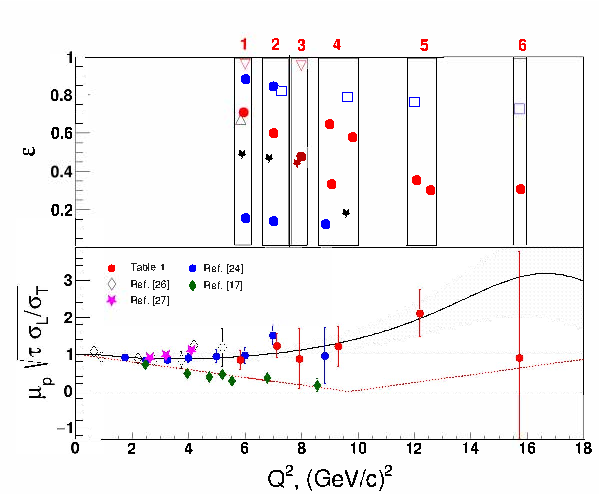
\includegraphics[trim = 0mm 0mm 0mm 40mm, width = 0.75\textwidth]{Plots/Fig1.pdf}
\caption{The square root of Rosenbluth slope, corrected for kinematical factor $\sqrt {\tau}$ and $\mu_p$, observed in elastic electron-proton scattering,
adopted from Ref.~\cite{Christy2020ab}.}
\label{pic:Fig1}
\end{figure}

The linear $\epsilon$ dependence of the cross section is due to $\sigma_{_L}$ term, see Eq.~\ref{eq:Ros}.
The ratio $\sigma_{_L}/\sigma_{_T}$ is a Rosenbluth slope related to \gef/\gmf (in OPE), see Fig.~\ref{pic:Fig1}.
The data show that at \qsq~of 4-5 \gevcsq~the Rosenbluth slope is three-four times larger than it suppose to be (in OPE) for
the observed values of the \gep/\gmp~ratio.

%
The nucleon electromagnetic form factors can reveal a lot of information about the nucleon internal structure, as well as the quark distribution. 
The form factors depend only on one variable the negative square of the four-momentum transfer carried by the photon, \qsq. 
In the limit of large \qsq, pQCD provides well-motivated predictions for the \qsq-dependance of the form factors and their ratio. 
However, it was never predicted at what \qsq~range the pQCD prediction (scaling) will be valid.
Studies of GPDs show that pQCD validity will require a very large \qsq~of 100~\gevcsq. 
It was discovered at JLab, using the double polarization methods, that the proton electric and magnetic form factors behave differently starting at \qsq~ $\approx$ 1~\gevcsq.
 
\begin{figure}[th]
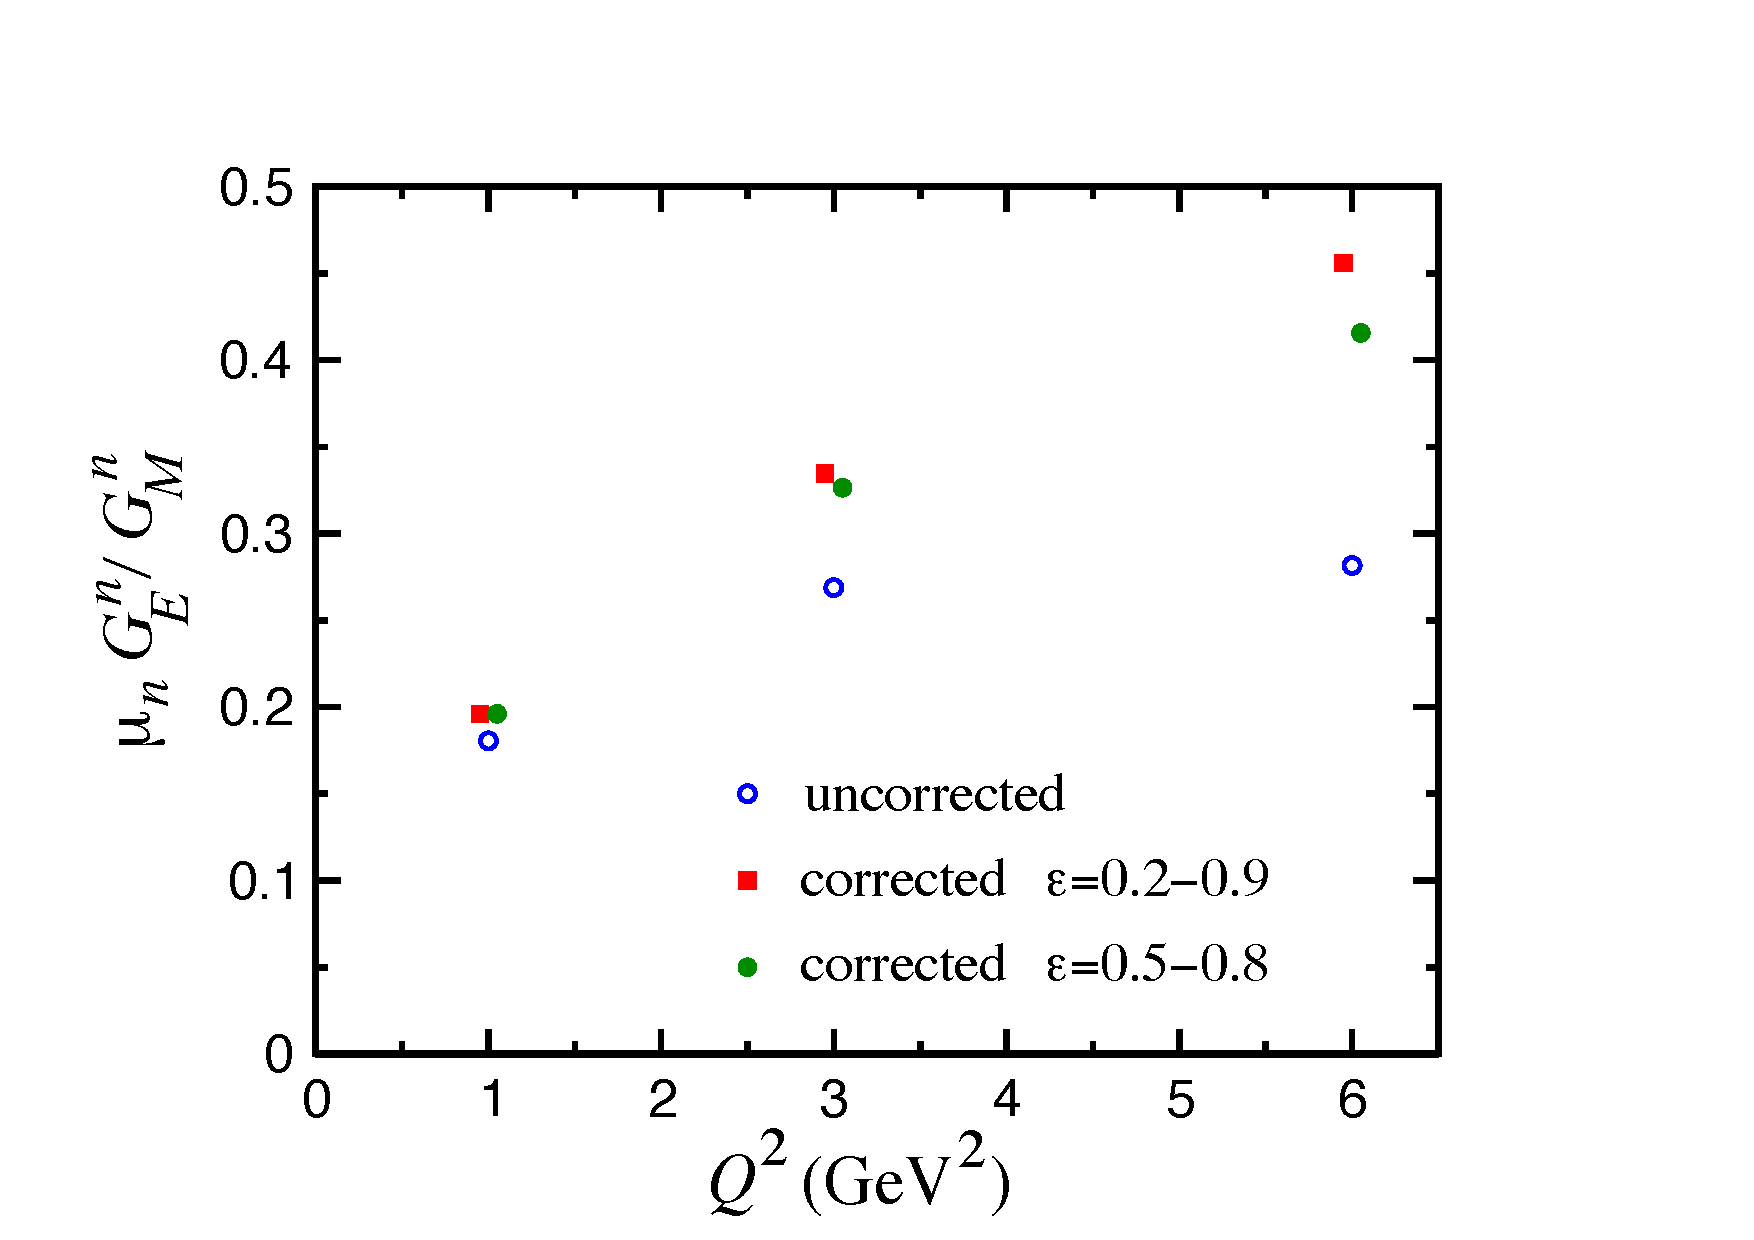
\includegraphics[width = 0.95\textwidth]{Plots/nTPE-BMT.pdf}
\caption{Projected impact of TPE on \gen/\gmn~using LT separation, according to Ref.~\cite{Blunden:2005ew}.}
\label{pic:Fig2}
\end{figure}
 
Experimentally, the nucleon form factors can be measured using one of two techniques: polarization transfer technique and Rosenbluth technique. 
The polarization method examines the polarization transfer from longitudinally polarized electron to the recoiling nucleon and 
determine the resulting azimuthal asymmetry distribution using a polarimeter. 
Alternatively, one can use the polarized  electron beam and a polarized target. 
While in the Rosenbluth method, the electric and magnetic from factors can be separated by making two or more measurements with 
different $\epsilon$ values ($i.e.$ different beam energies and angles), but with same \qsq~value. 
Rosenbluth technique requires an accurate measurement of the cross section and suffers from large systematic uncertainties arising from several factors. 
For instance, an accurate knowledge of the neutron detector efficiency is required.

When comparing the values of \gep/\gmp~obtained from both techniques, a significant discrepancy was observed (see Fig.~\ref{pic:Fig1}). 
Such discrepancy implies a potential problem in our understanding of the nucleon substructure. 
Many efforts were made in order to provide legitimate explanation, and it is believed that the inconsistency is due to contribution of two-photon exchange
in $e-N$ elastic scattering process, see Refs.~\cite{Arrington:2011dn, Afanasev:2017gsk}.
Predictions made for the neutron case are shown in Fig.~2
%\ref{pic:Fig2}
, adopted from~\cite{Blunden:2005ew}.
The contribution of TPE could reach about 30\% of Rosenbluth slope value at 5 \gevcsq.

In the following we propose to make precision L/T separation of the elastic electron-neutron cross section and first experimental assessment 
of the two-photon exchange contribution on the neutron magnetic form factor measurements (see also Ref.~\cite{Wojtsekhowski:2017kti}).
The result of the nTPE experiment will likely add a new component to our understanding of the elastic electron-nucleon process.

% June 10 9 am        do not change or remove this line
%
\section{Physics Motivation}

\indent
The nucleon plays the same central role in hadronic physics that the hydrogen atom does in atomic physics and the deuteron in the physics of nuclei.
The structure of the nucleon and its specific properties, such as charge, magnetic moment, size, mass; the elastic electron scattering form factors, resonances; and structure functions in DIS, are of fundamental scientific interest.
The isospin is a fundamental property of the nucleon, so both the proton and neutron investigations are important to do.
By using data on the proton and neutron form factors the flavour structure could be explored~\cite{Cates:2011pz}.
It is already provided the most direct evidence for a diquark correlation in the nucleon~\cite{Roberts:2007jh, Segovia:2014aza, Wojtsekhowski:2020tlo}.

Hadron structure, as seen in elastic electron scattering, in one-photon approximation, defined by two functions of four momentum transfer square.
They are: the helicity conserving Dirac form factor, $F_1$, which describes the distribution of the electric charge, and the helicity non-conserving Pauli form factor, $F_2$, describes the distribution of the magnetic moment.
These two form factors are the ingredients of the hadronic current.  
These form factors contain information on the transverse charge distribution for an unpolarized and transversely polarized nucleon, respectively, 
in the infinite momentum frame~\cite{Miller:2007uy, Carlson:2007xd}.

The Sachs form factors, \gef~and \gmf, the ratio of which will be extracted directly from the data, are related to $F_1$ and $F_2$ by
%
\begin{equation}
F_{1} = \frac{G_{E} + \tau G_{M}}{1+\tau} \mbox{  and  }
F_{2} = \frac{G_{M} - G_{E}}{\kappa (1+\tau)},
\label{eq:f1f2}
\end{equation}
%
where $\kappa$ is the nucleon anomalous magnetic moment.

Already twenty four years ago, important developments in QCD phenomenology has been the exploration of the generalized parton distribution (GPD) formalism~\cite{Mueller:1998fv, Ji:1996ek, Radyushkin:1996nd}, which provides relations between inclusive and exclusive observables.
The nucleon elastic form factors $F_1$ and $F_2$ are given by the first moments of the GPDs
%
\begin{equation}
F_1(t) = \sum_q \int^1_0 H^q (x,\xi,t,\mu) dx\ 
 \mbox{  and\  }
F_2(t) = \sum_q \int^1_0 E^q (x,\xi,t,\mu) dx,
\label{eq:F1/2}
\end{equation}
%
where $H^q$ and $E^q$ are two of the generalized parton distributions, $x$ is the standard Bjorken $x$, $\xi$ is is the ``skewdness'' of the reaction, $t$ is the four-momentum transferred by the electron, $\mu$ is a scale parameter necessary from the evolution over $Q^2$, analogous to DIS parton distributions, and the sum is over all quarks and anti-quarks.  
These may be accessed through processes such as deeply virtual Compton scattering, where the interaction is factorized into a hard part with the virtual photon/photon interactions with an individual quark and a soft part of the residual system where the GPD information is contained.

Fundamental nucleon feature, the spin, is related to GPDs, as shown by X.~Ji~\cite{Ji:1996ek}. 
The moments of GPDs can yield information, according to the Ji's Angular Momentum Sum Rule, 
on the contribution to the nucleon spin from quarks and gluons, including both the quark spin and orbital angular momentum.

At present, experimental measurements of GPDs are still scarce.  
Until high \qsq~DVCS data becomes available, work has been done to attempt to parameterize these GPDs,  
which rely heavily on data from electromagnetic form factors and parton distributions from DIS as constraints~\cite{Diehl:2013xca}.  
Data at high \qsq~for \gen~would contribute significantly in the development of these models.

As we presented above the form factors are important components for GPDs development.
However, the cross section of elastic $e-p$ scattering contains a significant contribution to $\sigma_{_L}$, 
which at high \qsq~is much larger than theory calculations expected~\cite{Kivel2020ab}.
Such an alarming observation underlines that understanding of TPE effect is essential for hadron physics. 
%

\section{Technique}
%
This proposal is based on instrumentation, simulation, and analysis development made by the GMn/SBS collaboration for the GMn, E12-09-019, experiment~\cite{E12-09-019}.
The GMn experiment is one of several form factor experiments approved by JLab PAC. 
The SBS spectrometer was funded by DOE with large contributions provided by the collaborating institutions from USA, Italy, UK, and Canada. 
The apparatus and DAQ installation will start in 2020 and the data taking run is expected to be in summer-fall 2021.

The neutron form factors are challenging to be determine experimentally especially because there is no free neutron target. 
However, since the deuterium is a loosely coupled system, it can be viewed as the sum of a proton target and a neutron target. 
In fact, quasi-elastic scattering from deuterium has been used to extract the neutron magnetic form factor, \gmn, at modestly high \qsq~for decades~\cite{Hughes:1965zza, Arnold:1988us} in the single arm (e,e') experiments. 
However, the proton cross section needs to be subtracted by applying a single-arm quasi-elastic electron-proton scattering. 
This ``proton-subtraction" technique suffers from a number systematic uncertainties e.g. contributions from inelastic and secondary scattering processes. 

Many year ago, L.~Durand~\cite{Durand:1959zz} proposed the so-called ``ratio-method" based on the measurement of both D(e,e'n) and D(e,e'p) reactions. 
In this method, many of the systematic errors are cancel out. 
Several experiments \cite{Bruins:1995ns, Kubon:2001rj, Lachniet:2008qf} have applied the ratio-method to determine the neutron magnetic form factor.

The GMn/SBS experiment~\cite{E12-09-019} will take data for elastic $e-n$ scattering for several kinematics with \qsq~from 3.5 up to 13.5~\gevcsq.
We propose to use this method to measure Rosenbluth slope and extract (in OPE approximation) the neutron electric form factor, \gen,~at one value of momentum transfer.
In fact, one of required data points will be taken by the GMn experiment, so an additional measurement is needed only for one
kinematics.

Data will be collected for quasi-elastic electron scattering from deuteron in process $D(e,e'n)p$. 
A complementary $D(e,e'p)n$ data will be taken to calibrate the experiment apparatus.
The current knowledge of the $e-p$ elastic scattering cross section (obtained in the single arm H(e,e')p and H(e,p)e' experiments) will be also used
for precision determination the experiment kinematics.

Applying Rosenbluth technique to measure \gen~requires accurate measurement of the cross section  and suffers from large uncertainties. 
To overcome this issue, we propose to extract the value of \gen~from the ratio of quasi-elastic yields, $R_{n/p}$, in scattering from a deuteron target as follows: 

\begin{equation}
R_{n/p} \equiv R_{observed} = \frac{N_{e,e'n}}{N_{e,e'p}}
\label{eq:1}
\end{equation}
$R_{observed}$ needs to be corrected to extract the ratio of e-n/e-p scattering from nucleons:

\begin{equation}
R_{corrected} = f_{corr} \times R_{observed} \;\; ,
\label{eq:2}
\end{equation}
where the correction factor $f_{correction}$ takes into account the variation in the hadron efficiencies due to changes of $e-N$ Jacobian, the radiative corrections, and absorption in path
from the target to the detector, and small re-scattering correction.

In one-photon approximation, $R_{corrected}$ can be presented as: 

\begin{equation}
R_{corrected} = \frac {\sigma_{_{_{Mott}}}^n \cdot (1+\tau_p)}{\sigma_{_{_{Mott}}}^p \cdot (1+\tau_n)} \times \frac{\epsilon \sigma_{_L}^n + \sigma_{_T}^n}{\epsilon \sigma_{_L}^p + \sigma_{_T}^p}
\end{equation}

It is important that the ratio $R_{Mott} = \frac {\sigma_{_{_{Mott}}}^n \cdot (1+\tau_p)}{\sigma_{_{_{Mott}}}^p \cdot (1+\tau_n)}$ could be determine with very high relative accuracy even with modest precision for the beam energy, electron scattering angle, and detector solid angle. 
Now, let us write the $R_{corrected}$ at two values of $\epsilon$ using $R_c^{n(p)} = \sigma_{_L}^{n(p)}/ \sigma_{_T}^{n(p)}$ as:
\begin{equation*}
R_{{corrected},\epsilon_1} = R_{Mott,\epsilon_1} \times \frac{\epsilon_1 \sigma_{_L}^n + \sigma_{_T}^n}{\epsilon_1 \sigma_{_L}^p + \sigma_{_T}^p}
\hskip .5 in
R_{{corrected},\epsilon_2} = R_{Mott,\epsilon_2} \times \frac{\epsilon_2 \sigma_{_L}^n + \sigma_{_T}^n}{\epsilon_2 \sigma_{_L}^p + \sigma_{_T}^p}
\end{equation*}

In these two equations there are two unknown variables: $\sigma_{_L}^n$ and $\sigma_{_T}^n$.
The dominant contribution to the uncertainty of the slope of the cross section vs. $\epsilon$,  
$S_c^n = \sigma_{_L}^n/ \sigma_{_T}^n$, will come from the uncertainty of $S_c^p$.
At \qsq=4.5 \gevcsq, according to the global analysis of $e-p$ cross section~\cite{Christy2020ab}, the value of $S_c^p$ is close to $1/(\tau \, \mu_p^2) = 0.107$ with uncertainty of 0.01.
The resulting equation for $S_c^n$ is:
\begin{equation*}
A = B \times \frac{1 + \epsilon_1 S_c^n}{1 + \epsilon_2 S_c^n} \approx B \times (1 +  \Delta \epsilon \cdot S_c^n),
\end{equation*}

where the variable $A = R_{{corrected},\epsilon_1}/R_{{corrected},\epsilon_2}$ will be measured with relative precision of 0.1\%.  
Assuming, for this estimate, equal values of \qsq~for two kinematics, the  $\tau$ and $\sigma_{_T}$ for two kinematics are canceled out, and the variable
\mbox{$ B = {R_{M,\epsilon_1}}/{R_{M,\epsilon_2}} \times (1+ \epsilon_2 \, S_c^p)/( 1 + \epsilon_1 \, S_c^p)$}.
For actual small range of $\epsilon$ and small value of the slope, the $B \approx (1 - \Delta \epsilon \cdot S_c^p)$.
The value of B will be determined from global proton $e-p$ data to a precision of $0.25 \times 0.01$.
 
At \qsq=4.5 \gevcsq~the ratio $\mu_n$\gen/\gmn~is of $0.55 \pm 0.05$, see the review~\cite{Punjabi:2015bba}.
%
In a simplest model, the slope $S_c^n$ is a sum of the slope due to \gen/\gmn~and the TPE contribution.
If we use for TPE the prediction~\cite{Blunden:2005ew}, shown in Fig.~2, the TPE leads to increase of $S_c^n$ by a factor of 2,
so the result of this experiment for TPE will be $0.069 \pm 0.012 \pm 0.01$, where the first uncertainty is due to accuracy 
of \gen/\gmn~and the second one due to projected precision of this experiment. It would be a 4-4.5 sigma observation of the neutron TPE.

\section{Proposed Measurements} 
\label{prop}

We propose to use the same experimental setup of the E12-09-019 experiment. We will add a kinematic point at \qsq~= 4.5 \gevcsq, at a higher beam pass (6.6~GeV/3~pass instead of 4.4~GeV/2~pass), leading to a higher $\epsilon$ value. This additional point along with the data point of the E12-09-019 experiment will allow us to perform the standard Rosenbluth method to obtain (in one-photon approximation) the neutron electric and magnetic form factors. In addition, the ratio method (Sec.\ref{sec:exp_method}), in which the systematic errors are greatly reduced, will be implemented to calculate  the two photon exchange (TPE) contribution. The study of the $\epsilon$ dependance two photon exchange contribution to the neutron form factor ratio \gen/\gmn. Table.~I displays the kinematic settings of the proposed experiment. 

\begin{table}[h] 
\centering
\begin{tabular}{|c|c|c|c|c|c|c|}
\hline
\small{Point} & $Q\textsuperscript{2}$  & E & E$'$  & $\theta_{BB}$ & $\theta_{SBS}$ & $\epsilon$ \\
& (GeV/c)$^2$ & (GeV) & (GeV)  &\; degrees\; & \; degrees \;  &   \\
\hline
\textcolor{blue}
 1&\textcolor{blue} {4.5} & \textcolor{blue}{4.4} & \textcolor{blue}{2.0} & \textcolor{blue}{41.88}  & \textcolor{blue}{24.67} &\; \textcolor{blue}{0.599} \;\\
\hline
2 & 4.5  &  6.6  &  4.2  & 23.23  &  31.2  &  0.838 \\
\hline
\end{tabular} 
\caption{Kinematic settings of the proposed experiment. The kinematic point with the lowest $\epsilon$ value (blue raw) is an existing measurement of the approved  E12-09-019 experiment.}
\label{tab:propkin}
\end{table}


% v 1.9
\section{Experimental Setup}
%
\label{sec:expsetup}

As illustrated in Fig.~3, this experiment will study electron scattering from a 15 cm long 
liquid Deuterium target held in a vacuum.
The scattered electron will be detected in the BigBite spectrometer with an upgraded electron detector stack. 
The neutron arm is arranged with a dipole magnet 48D48 (SBS) and a segmented hadron calorimeter HCAL.  
The whole detector package was designed and is now under assembling for the GMn, E12-09-019, experiment. 

\begin{figure}[bh]
	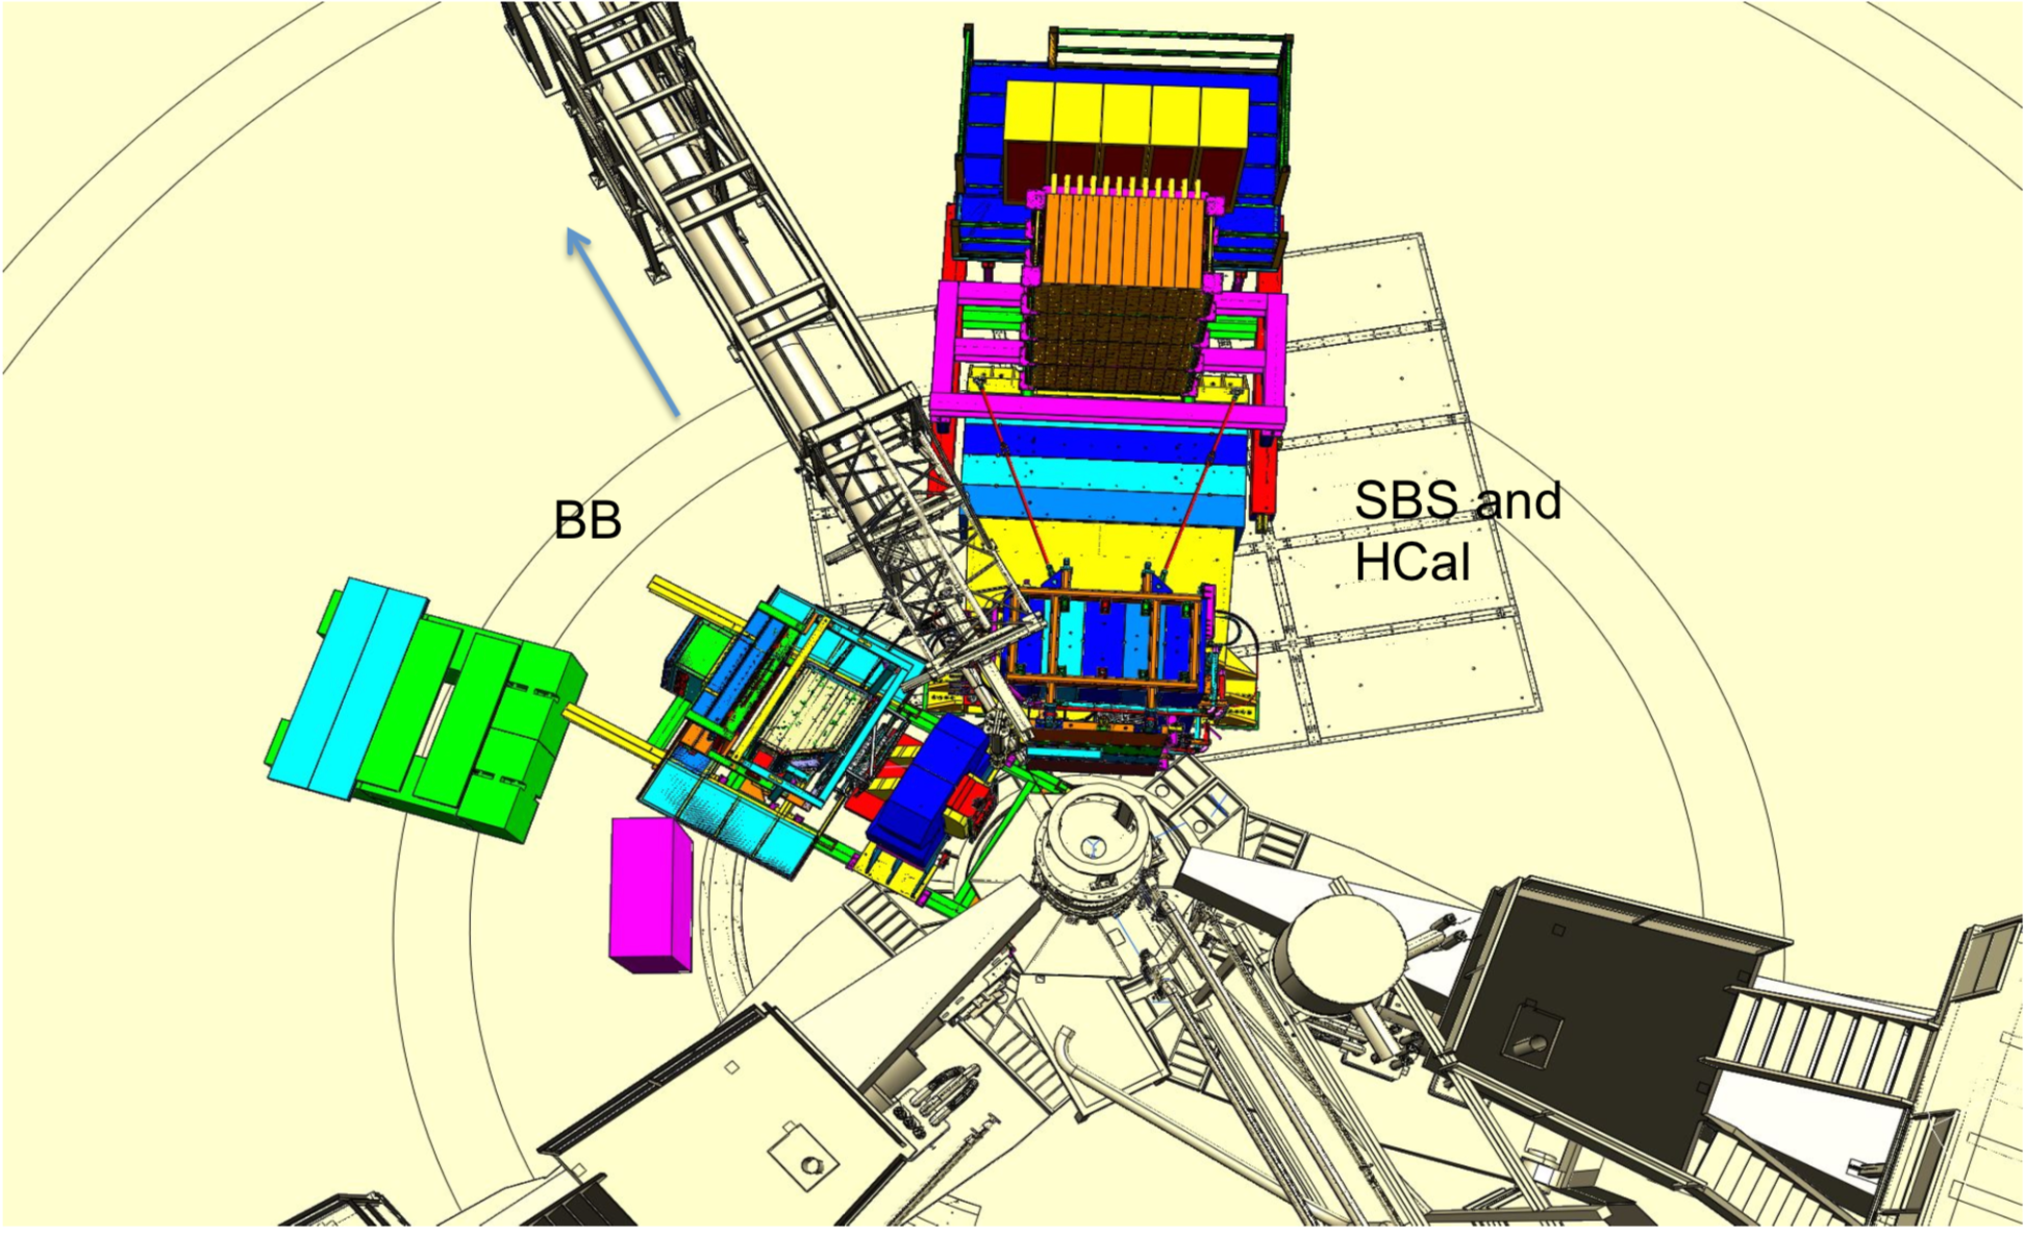
\epsfig{file=Plots/Exp_setup_3D.pdf, height=3.0in}
	\caption{Layout of the experimental setup in nTPE.}	
\label{pic:expsetup}
\end{figure}

\subsubsection{Parameters of the SBS}

The 48D48 magnet from Brookhaven was acquired as part of the Super Bigbite project and will be available for this experiment.  
It consists of a large dipole magnet which provides a field integral of about 1.7~ T $\cdot$ m, allowing for quasielastic 
protons to be sufficiently deflected to allow clear differentiation from neutrons.  
The active field volume has an opening of $46 \times$ 25 vertical $\times$ horizontal), 
matching the aspect ratio of the neutron arm, and a depth of 48 cm.

The placement of this magnet will be 1.6 m away from the target, which would normally interfere with the beamline.  
To accommodate this, modifications were made to the iron yoke such that the beamline will pass through the magnet yoke area.

The field configuration will be such that positively charged particles will be deflected upwards away from the hall floor.  
For a field integral of 1.7 Tesla-m, protons of momentum 2.5 GeV/c will be deflected 250 mrad,
 which translates to a displacement of xxm.  
 Including expected detector resolution,  the $p_{miss,\perp}$ distribution will be similar to 
 what was seen in E02-013, so cuts of  $< 100$ MeV/c will be appropriate.  
Monte Carlo simulations show a contamination of charged quasielastics to be negligible.

The presence of the magnet also works to sweep low energy charged particles from the target away from the neutron arm.  
Particles of momentum less than 1.3~{GeV/c} will be entirely swept outside of the neutron arm acceptance.  
This greatly reduces the amount of charged low energy background.
%


%%v4.4
\subsection{The BigBite Spectrometer}
%
\label{sec:expsetup_bigbite}             
%
Scattered electrons will be detected in the BigBite spectrometer.
The spectrometer consists of a single dipole magnet (with magnetic field approximately 1.2~Tesla-m 
and a detection system, see Fig.~4.  

\begin{figure}[htbp]
\begin{center}
%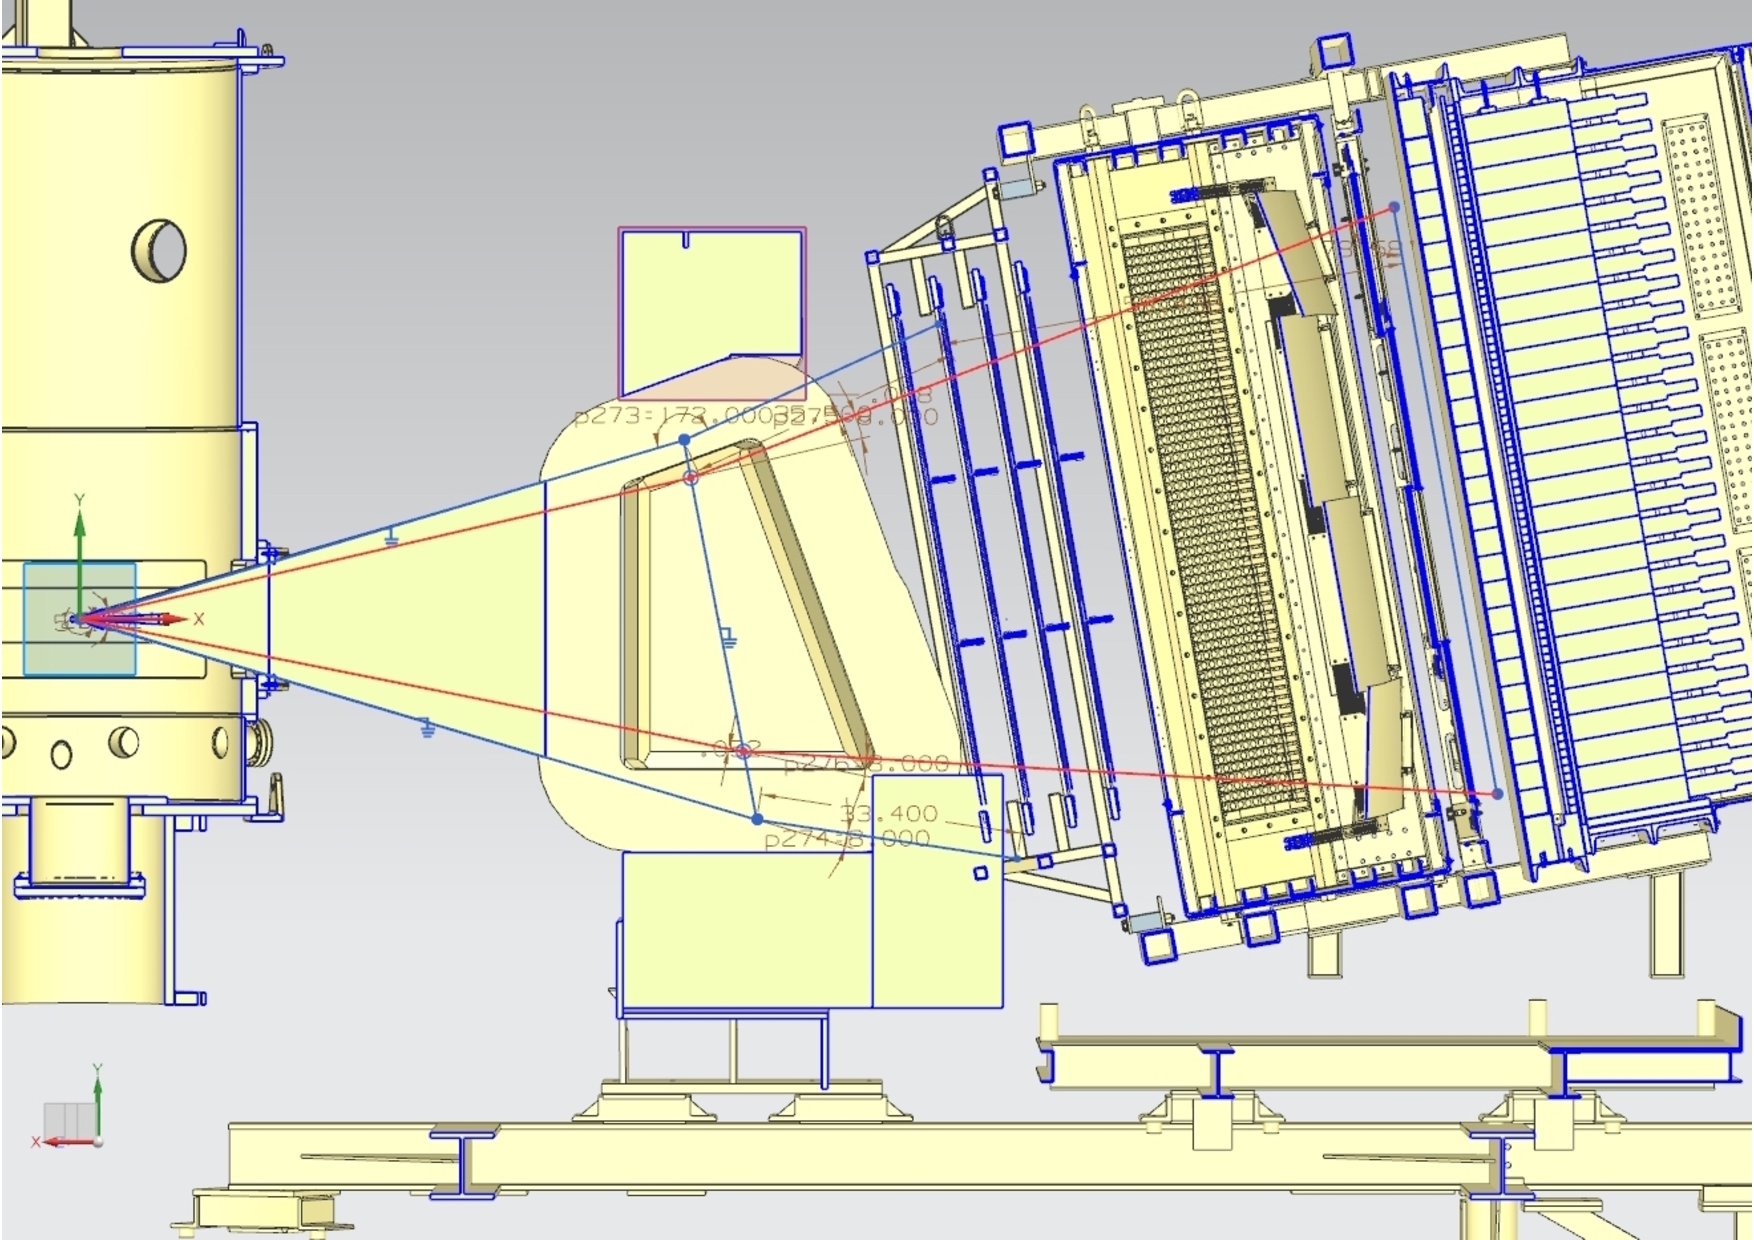
\includegraphics[trim = 5mm 0mm 0mm 0mm, width=0.475\textwidth, angle = 0]{Plots/BB_Side-view.pdf} 
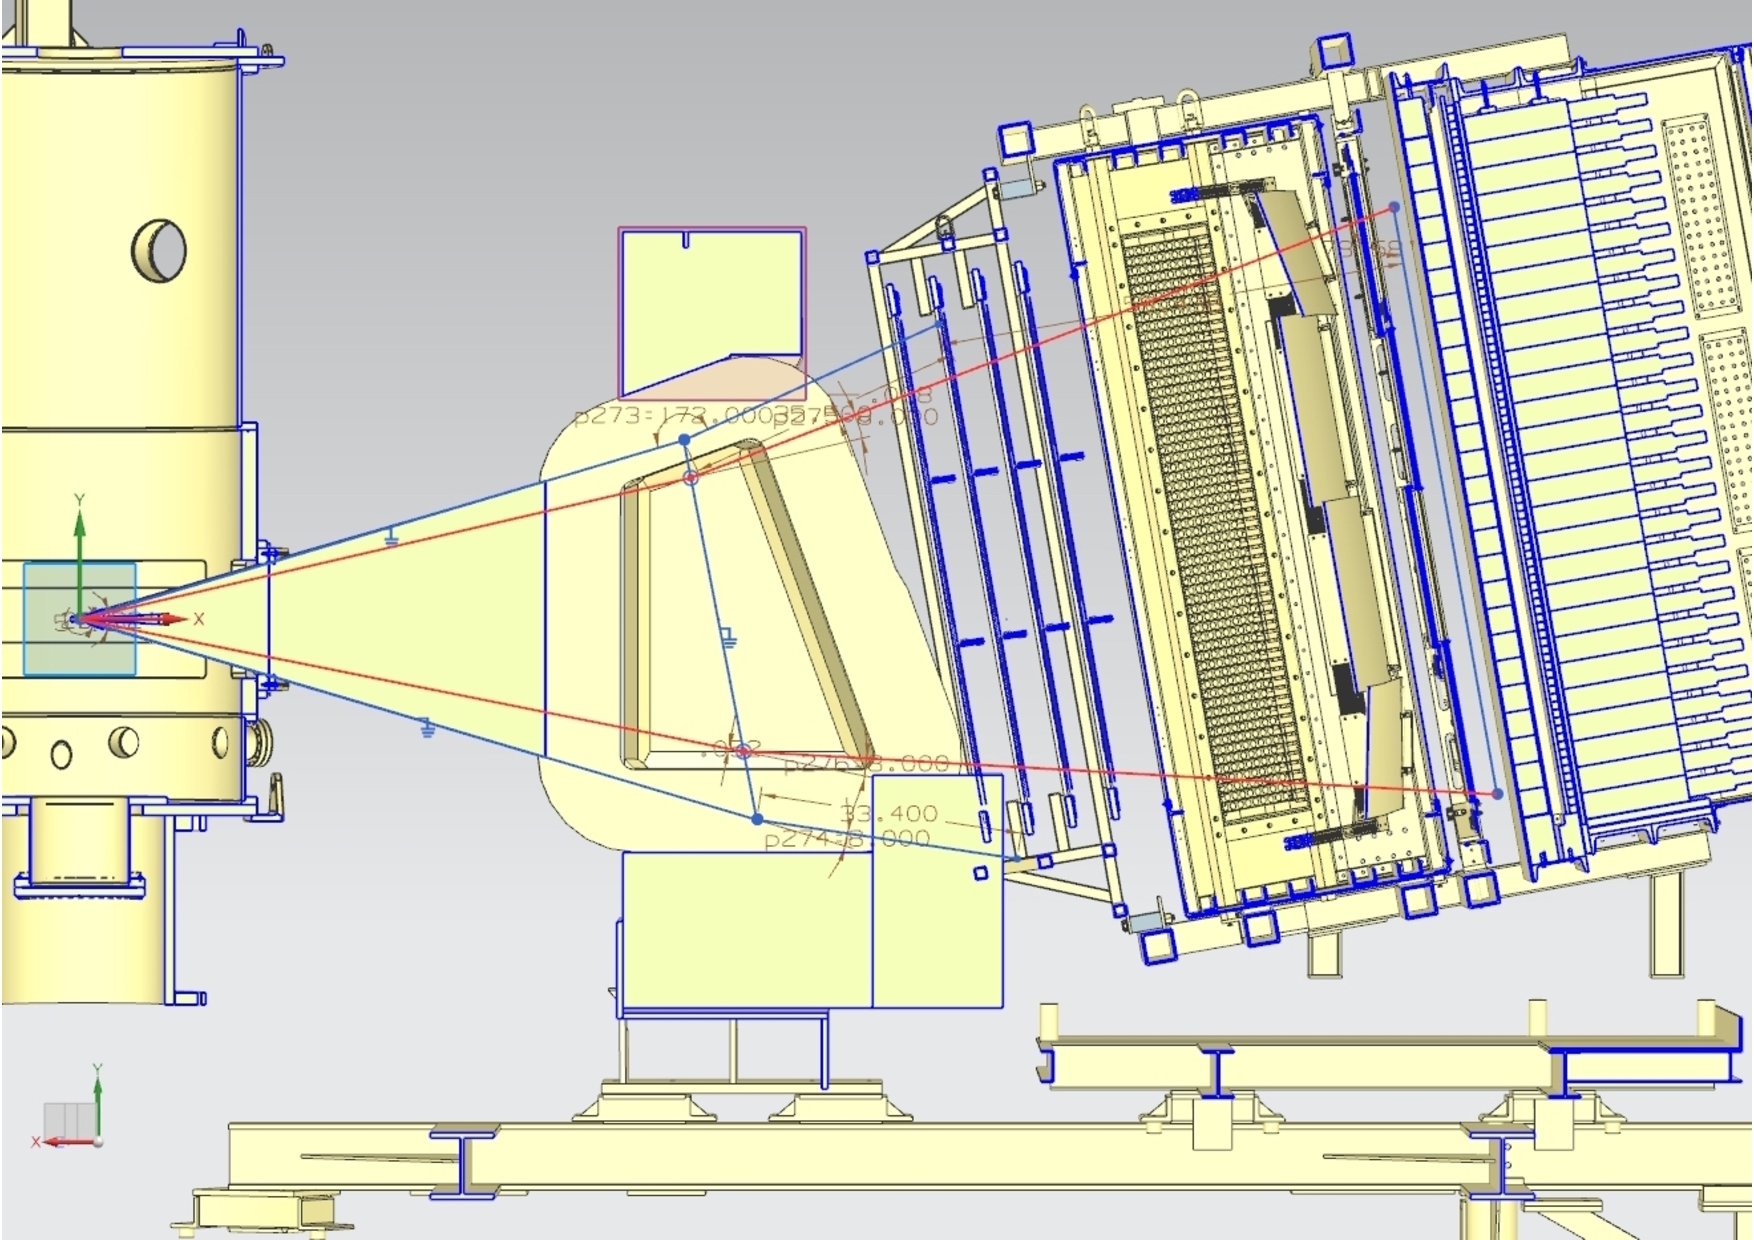
\epsfig{file=Plots/BB_Side-view.pdf, height=3.0in}
\end{center}
\caption{The BigBite spectrometer with the upgraded detector stack.}
\label{fig:BB}
\end{figure} 

\subsubsection{Simulation of BigBite}

\subsubsection{Detector Package}

\paragraph{Background Rate in BigBite}

\paragraph{Front GEM chambers}

\paragraph{Gas Cherenkov Counter}

\paragraph{Rear GEM chamber}

\paragraph{Shower and Preshower}

\paragraph{Timing Scintillator Hodoscope}

\subsubsection{Trigger}

\subsubsection{Simulation of BigBite}

\paragraph{Rates in the detectors}

\paragraph{Trigger rate and efficiency}
%%v4.4
\subsection{Neutron Detector}
%
\label{sec:expsetup_neutron}
  s

\subsubsection{Structure of the Neutron Detector}


%v4.4
\subsection{The BigBite Spectrometer}
%
\label{sec:expsetup_bigbite}             
%
Scattered electrons will be detected in the BigBite spectrometer.
The spectrometer consists of a single dipole magnet (with magnetic field approximately $1.2~\mathrm{T}$) and a detection system, see Fig.~\ref{fig:BB}.  

\begin{figure}[htbp]
\begin{center}
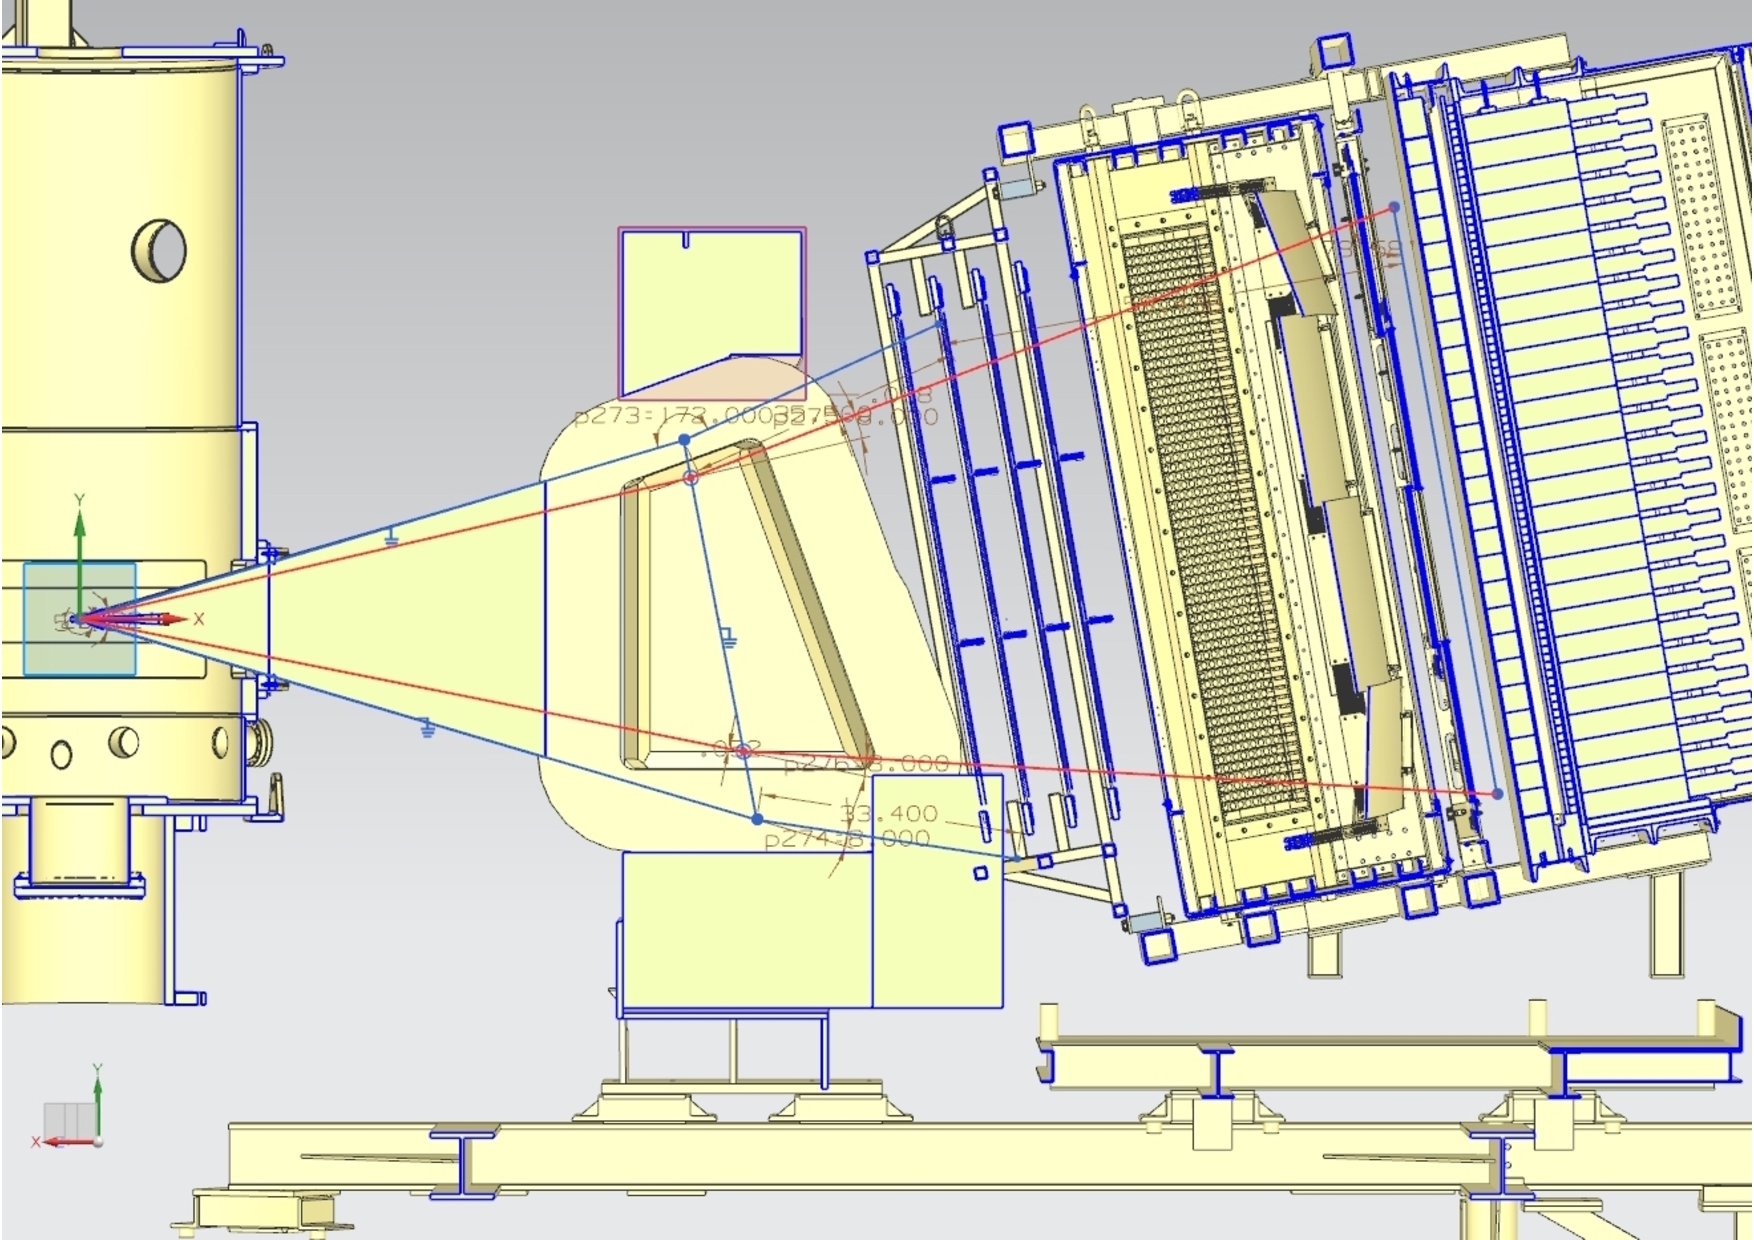
\epsfig{file=Plots/BB_Side-view.pdf,height=3.0in}
\end{center}
\caption{The BigBite spectrometer with the upgraded detector stack.}
\label{fig:BB}
\end{figure} 

\subsubsection{GEM Chambers}
To perform the tracking of charged particles under the high rates anticipated for this experiment, the drift chambers were replaced with gas electron multiplier (GEM) detectors.  
These detectors have proven to be capable of operating under luminosities of $25~\mathrm{kHz/mm}^2$ for the COMPASS experiment at CERN and the spatial resolution of each of these chambers is anticipated to be about $70~\mathrm{\mu m}$.
There will be two sets of GEMs placed on each side of the GRINCH Cherenkov detector.

The set of GEMs in front of the GRINCH is composed of four layers of GEMs.
Two of these layers have been built by will the SBS collaborators from INFN.
They are composed three modules each, measuring $40~\times~50~\mathrm{cm}^2$, such that each layer covers $40~\times~150~\mathrm{cm}^2$ (the long dimension being vertical, along the dispersive direction). The readout of these modules are oriented in the $x/y$ direction {\it i.e.} parallel and perpendicular to the dispersive direction (horizontal and vertical).
The two other layers are being built by the SBS collaborators from UVA. They are composed of a single module measuring $40~\times~150~\mathrm{cm}^2$, the long dimension again being vertical and along the dispersive direction.
The readout of these modules are oriented in the $u/v$ direction {\it i.e.} $\pm~30$~degrees with respect to the horizontal direction.

The set of GEMs behind the GRINCH has been been built by the SBS collaborators from UVA. It is composed of a single layer composed of four modules measuring $50~\times~60~\mathrm{cm}^2$ , such that the layer covers $60~\times~200~\mathrm{cm}^2$ (the long dimension again being along the dispersive direction).
The readout of these modules are all oriented in the $x/y$ direction.

\iffalse
On Fig.~\ref{fig:uva_gem} is displayed the single back GEM layer.
%
\begin{figure}[!h]
  \begin{center}
    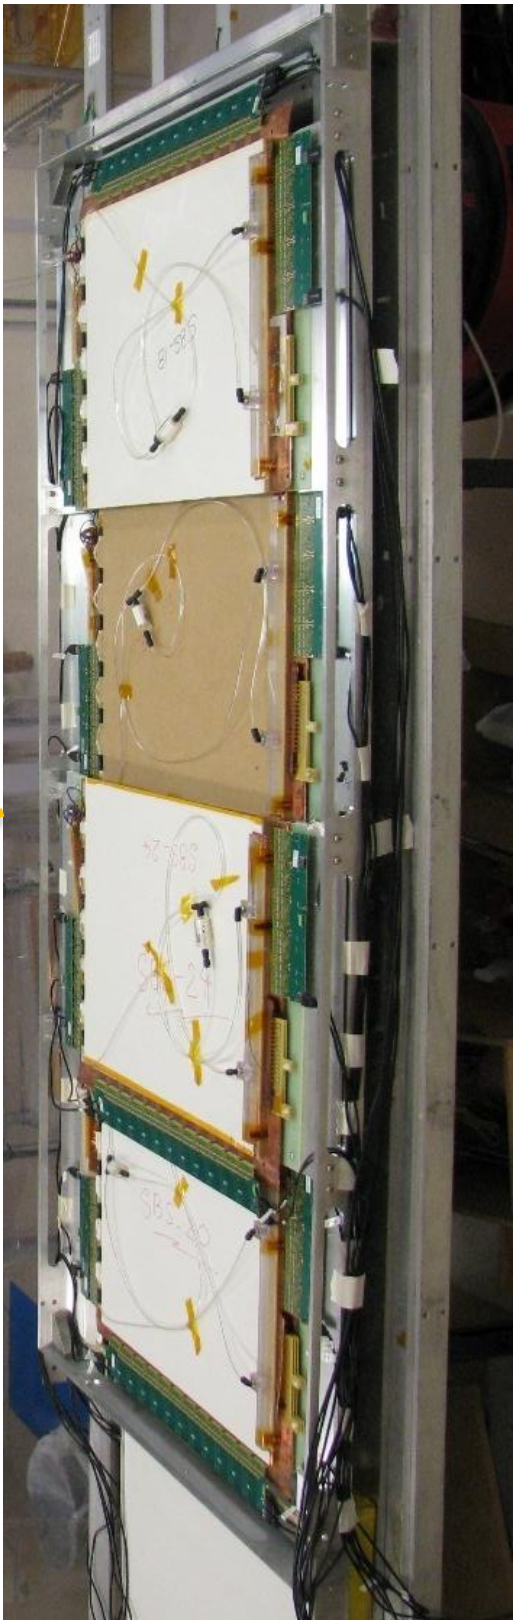
\includegraphics[angle=-90,width=10cm]{Plots/UVaGEMs.png}
    \caption{Picture of the back layer of GEMs, illustrating its arrangment}
    \label{fig:uva_gem}
  \end{center}
\end{figure}
%

For two sets of GEM chambers separated by a distance $z_\mathrm{GEM}$ and including multiple scattering effects, the angular resolution can be approximated by 
\begin{equation}
\left( \delta \theta \right)^2 = \frac{\sigma_x^2}{z_\mathrm{GEM}^2} + \left(\frac{13.6~\mathrm{MeV}}{\beta c p} \sqrt{x/X_0} \left[1+0.038\ln(x/X_0)\right]  \right)^2
\end{equation}
where $\beta c$ is the velocity of the electron, $p$ is the momentum of the electron, and $x/X_0$ is the thickness of the scattering material in radiation lengths.

For small deflection angles from a dipole magnet, the deflection angle, $\theta$, and the momentum, $p$, are related by the equation
\begin{equation}
p = \frac{ e \int B_\perp \cdot dl}{\theta},
\end{equation}
where $\int B_\perp \cdot dl$ is the field integral for the path of the electron.  
For electrons of momentum $3\sim4~\mathrm{GeV}$ and a field integral of $1.0~\mathrm{T\cdot m}$, this would yield a typical momentum resolution of $\delta p/p \approx 0.5\%$.

In order for us to accurately determine the scattered electron's angular
coordinates, momentum, and the position of the scattering vertex along the target, the optics of BigBite need to be studied.  
Data from a multi-foil carbon target and a removable lead sieve located 
at the front face of the magnet provide an accurate method to calibrate the angular coordinates 
before magnetic deflection and a beamline scattering vertex position.  
Data from elastic coincidence $ep$ scattering from a $\mathrm{H_2}$ target will provide data to calibrate the electron momentum and will be performed for each beam energy setting.  
As the kinematics for quasielastic and elastic scattering are similar, this provides the most efficient and reliable method for calibration.  
With the sieve plate in place, it also eliminates the need for $B=0$ field data, which was proven difficult to extract due to prohibitively high rates of otherwise deflected low energy particles.
\fi

The level background in the GEMs have been evaluated, thanks to G4SBS (\cite{g4sbs} and Sec.~\ref{sec:simu}) for the $G_M^n$ experimental readiness review. % \cite{gmn_err}.
For the $G_M^n$ highest $Q^2$ point (which is the most constraining, since it combines mandatory maximum luminosity and smaller BigBite angles, the background level in the front GEMs are of the order of $120~\mathrm{kHz/cm}^2$ for the front GEM layers, and below $50~\mathrm{kHz/cm}^2$ for the back GEM.
To perform the GEM tracking within such a background environment, we use the cluster reconstructed in the BigBite shower as a track seed to clean the large combinatorics that would otherwise be created by the large number of hits. After this, the main challenge is the separation by the clustering algorithm of the signal and background hits to minimize track smearing.
At this level of background, a TreeSearch tracking algorithm combined with a fairly simple cluster separation algorithm has already proven to achieve 70\% efficiency at nominal luminosity.
A better cluster separation algorithm is currently being developed and should allow to significantly improve this figure. 

\iffalse
\subsubsection{Simulation of BigBite}

Two packages of programs for the simulation of the BigBite spectrometer characteristics
were developed independently by V. Nelyubin \cite{nel01} and S.~Riordan.  
For this experiment, the momentum of the scattered electrons will be approximately $\mathrm{3.5~\mathrm{GeV/c}}$ for the $Q^2 = 10~\mathrm{GeV}^2$ point, 
leading to an expected momentum resolution of $\delta$p/p  of about 0.5\%.  
The expected position resolution on target
along the beam is $\sigma$= 4 mm, and the expected angular resolution in both 
scattering planes is better than $\sigma$=0.3 mrad.  

Additional MC studies were done to evaluate the parameters of the proposed experiment.  
The range of \qsq~accepted by the electron arm is shown in Fig.~\ref{pic:mom_range}. 
The solid angle of the electron arm for different positions along the target is shown in Fig.~\ref{pic:solidangle}.  
The average solid angle for our maximum electron energy is about 44 msr.
%

\subsubsection{Background Rate in BigBite}

Several MC simulations~\cite{pavel} and real data sets~\cite{riordan} were used for the calculation of the 
rate on the BigBite detectors. 
%
Charged particles with momenta below 300 MeV/c
will be deflected entirely out of the acceptance by the BigBite dipole. 
The majority of charged background particles with momentum above 300 MeV/c are $\pi^-$, and for pions near quasielastic 
electron momentum, are about a factor of 3 higher in rate than electrons (Sec.~\ref{sec:bbpion}).  
With an overall pion rejection factor of 10000:1, this number can be reduced to a negligible amount.

The total trigger rate on the shower/preshower with a threshold of $1.7~\mathrm{GeV}$ is expected to be about $2~\mathrm{kHz}$ from a simulation based on pion production rates from a parameterization done by Wiser~\cite{wiser}, Fig.~\ref{pic:rates}.  
This simulation when compared to the previous $G_E^n$ experiment predicted rates higher by a factor of 5, so this produces an upper limit on expected rates.  
Furthermore, adding the Cerenkov into the trigger configuration to explicitly reject pions and photons will be possible if necessary.

A majority of hits in the GEM chambers will be produced by photons.  
To investigate the photon detection probability a separate GEANT-4 code was used. 
The GEM geometry and materials were chosen to be the same as in the COMPASS chambers.
The probability to produce a secondary electron in the drift gap of the chamber as a function
of the energy of the initial soft photon is shown in Fig.~\ref{pic:gemphotons}. It is about $10^{-3}$ at 100 keV and
increases up to $4\times10^{-3}$ at 1 MeV. 
Above 1 MeV the photon efficiency (Fig.~\ref{pic:gemphotons2}) increases but doesn’t exceed 1\%. In the same figures, bottom panels, the probability for correlated
hits in two or more chambers is shown. 
This happens when one photon produces secondary electrons in several chambers. 
One can see that such a probability is negligible for photon energies below 1 MeV, and the hit rates on the chambers are dominated by uncorrelated
random hits.

Using data from the Transversity experiment, E06-010, which placed BigBite at $30^\circ$ at
$1.5~\mathrm{m}$ with a beam current of $12~\mathrm{\mu A}$, the rate per $140~\mathrm{cm}\times35~\mathrm{cm}$ chamber was $41~\mathrm{MHz}$.  
At our beam energies, beam current, active area, target length, and BigBite distance, we expect an increase in rate by about a factor of 13.  
Estimating the BigBite drift chamber photon efficiency to be at most a factor of 5 smaller than the GEM chambers, 
we anticipate an overall increase in the observed rate in the drift chambers to be a factor of 65, or a rate
of $4.5~\mathrm{kHz/mm^2}$. 
This is below rates in which these have been demonstrated to operate.
Using information from the shower and scintillator, the area in the GEM chambers to search for tracks can be restricted
 by a factor of 10, leading to approximately 26 false hits in a $100~\mathrm{ns}$ time window per plane.  
Current transversity tracking code operates with a time window larger by a factor of three
and without using shower information, presenting an overall background rate the tracking must
contend with higher by only a factor of two.  
This should present no problem for current BigBite tracking software.

Using rates of charged particles above $300~\mathrm{MeV}$, less than 20\% of events are anticipated 
to have multiple tracks in the same region as the triggering track.  
The $x$ and $y$ components of  these tracks can be separated using the fixed $z$ plane positions given by the shower and scintillator plane.
\fi

\subsubsection{Shower/Preshower}

The electromagnetic calorimeter configuration consists of two planes of lead glass blocks which  which we call the preshower and shower.  
The preshower, located about $80~\mathrm{cm}$ behind the first GEM chamber, consists of a $2\times26$ plane of $37~\mathrm{cm}\times 9~\mathrm{cm}$ blocks.  
The shower, about $1~\mathrm{m}$ behind the first GEM chamber, consists of an $7\times27$ array of $8.5~\mathrm{cm}\times8.5~\mathrm{cm}$ blocks.  Sums over these blocks form the physics event trigger for the experiment.

The preshower signal can be used to provide an additional method of pion rejection.  
By selecting low preshower signals, a pion rejection factor of 1:50 can be achieved through optimization.  
Despite higher particle rates, pion rejection performance is anticipated to be similar to that achieved for Transversity, E06-010.  
By measuring the pedestal widths and resolution for E06-010 and scaling to this proposal's conditions, overall relative energy resolution for the detector is expected to become worse by a factor of $1.6$, to about $\sigma_{\delta E/E} = 25\%$.

\subsubsection{Timing hodoscope}

The BigBite timing hodoscope has been built the the SBS collaborators from Glasgow, to replace the BigBite scintillator plane.
It will be composed of 90 bars stacked in a plane, each with dimensions $1~\mathrm{in.}\times1~\mathrm{in.}\times60~\mathrm{cm}$. The paddle stack will be oriented such as the long dimension of the bars is horizontal {\it i.e.} perpendicular to the dispersive direction.
Each of these elements are readout by a PMT on each side, mostly to provide measurement redundancy.

\iffalse
The arrangement of these elements can be visulaized on Fig.~\ref{fig:hodo}
%
\begin{figure}[!h]
  \begin{center}
    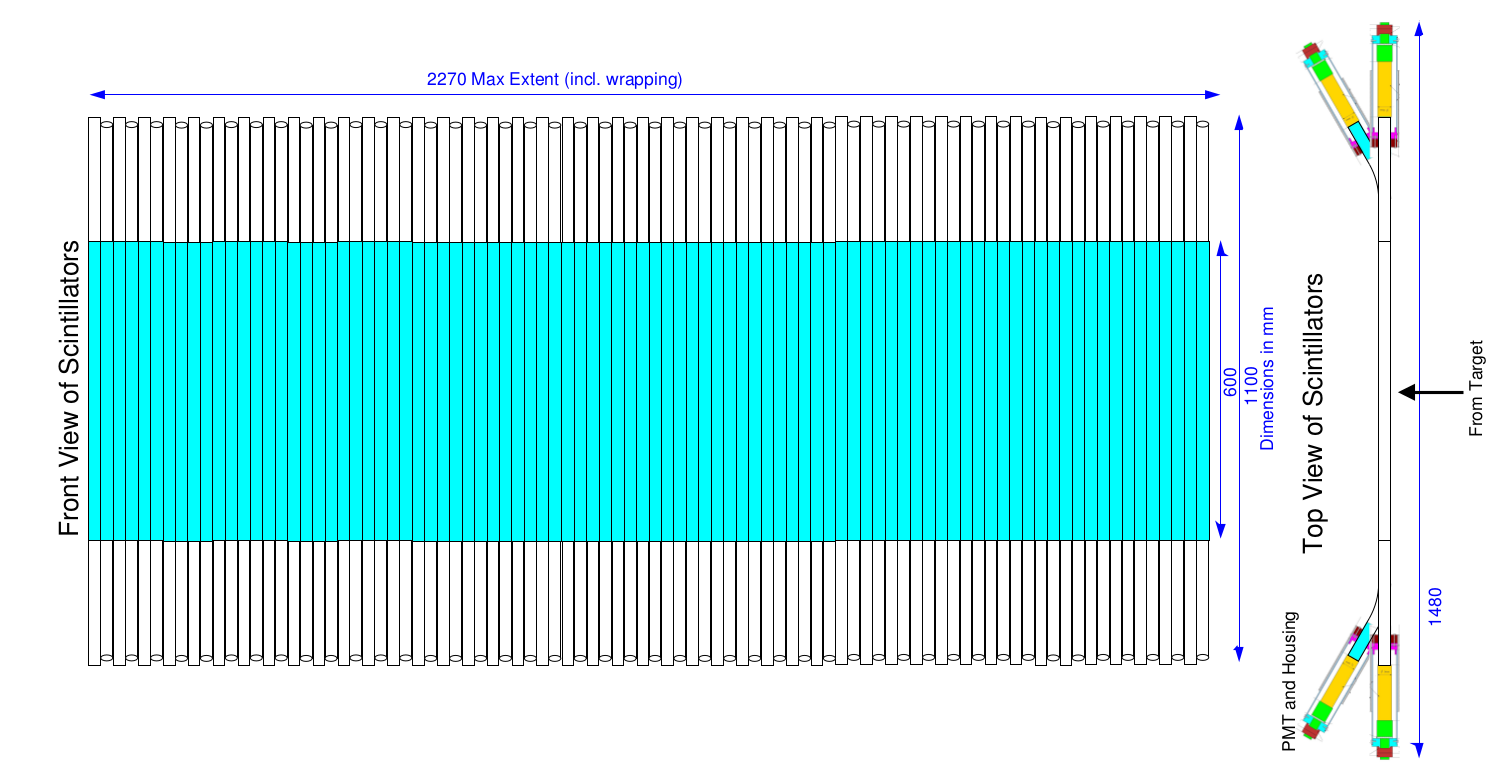
\includegraphics[angle=-90,width=5cm]{Plots/Hodo.png}
    \caption{Arrangement of the timing hodoscope elements.}
    \label{fig:grinch}
  \end{center}
\end{figure}
%
\fi
This plane will primarily be used to provide a signal for nucleon time of flight reconstruction. A time resolution of $200~\mathrm{ps}$ is anticipated.
%For the transversity experiment, where BigBite is at $30^\circ$ using a shorter $40~\mathrm{cm}$ \he~target, and $12~\mathrm{\mu A}$ beam, the rate
This fine segmentation is meant to lower the rates in the detector. Background studies made for the $G_M^n$ experimental readiness review %\cite{gmn_err}
demonstrated that the rates experienced by each element was $\leq~500~\mathrm{kHz}$ at a luminosity of $2.8~\times10^{38}~\mathrm{cm}^{-2}~\mathrm{s}^{-2}$. %for for the scintillator plane was approximately $3.6~\mathrm{MHz}$.
%Using this data to provide upper limits on the rates seen for our experiment, scaling to current, a longer target, and bar active area, we anticipate a rate of $270~\mathrm{kHz}$ per bar.  
The PMTs pulses are processed by NINO front-end cards which, when the PMT pulse crosses the NINO threshold, will produce a digital signal to be readout by CAEN 1190 TDCs which record a leading time and a trailing time.

\subsubsection{GRINCH cherenkov detector}

The main purpose of the Ring Imaging Cherenkov is to provide additional particle identification for offline pion rejection.
The GRINCH consists of a tank with a maximum depth of $88.9~\mathrm{cm}$, with 4 cylindrical mirrors focussing the cherenkov light directly onto a 510~PMT array (60 lines of PMTs, with lines of 9~PMTs alternating with lines of 8~PMTs) placed away from the beam.
\iffalse
The GRINCH tank and PMT matrix are represented on Fig.~\ref{fig:grinch}
%
\begin{figure}[!h]
  \begin{center}
    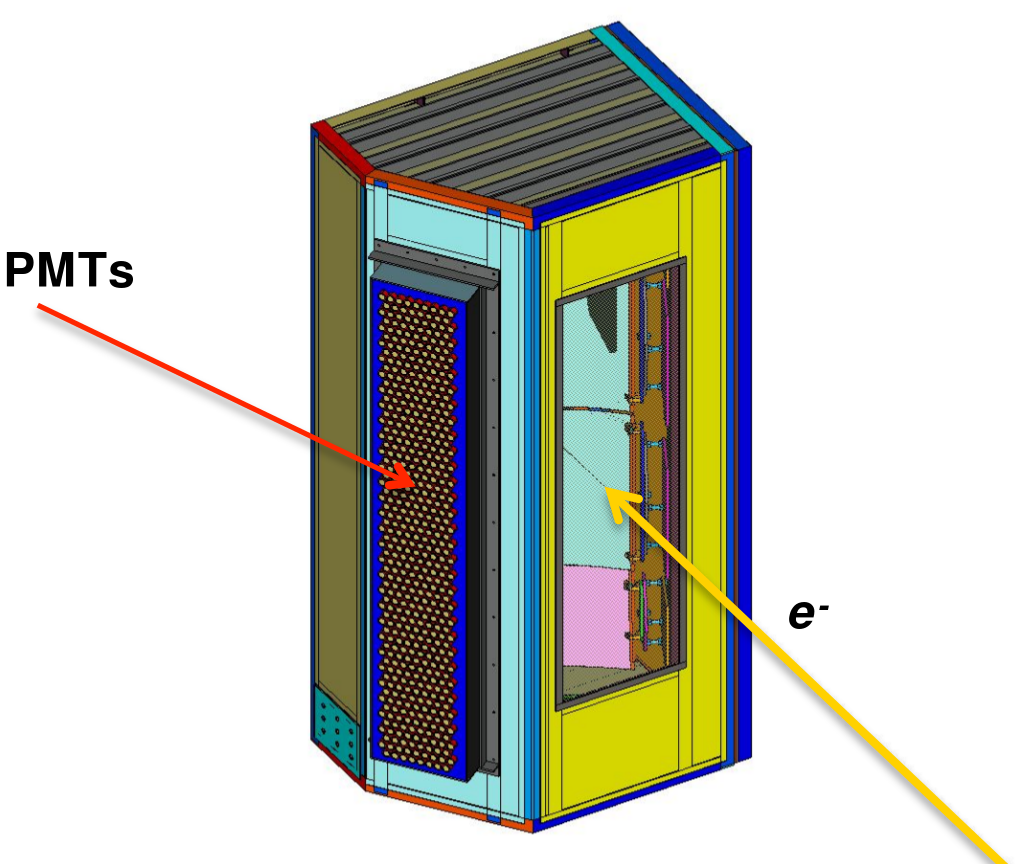
\includegraphics[width=6cm]{Plots/GRINCH.png}
    \caption{CAD representation of the GRINCH tank and PMT matrix}
    \label{fig:grinch}
  \end{center}
\end{figure}
%
\fi
The radiation gas will be $C_4F_8$, which is by far the best compromise between light yield for electrons and operating cost.
With $n-1=1.35\times10^{-3}$, the $\pi$ threshold is only about $2.7~\mathrm{GeV}$, so the additional pion rejection will be most effective below this threshold. 

As for the timing hodoscope The PMTs pulses are processed by NINO front-end cards which, when the PMT pulse crosses the NINO threshold, will produce a digital signal to be readout by VETROC TDCs, which for each PMT hit will record a leading time and a trailing time.
The analog signal will not be recorded however, which means that for each PMT hit, the information of the number of not directly available (although it can in theory be deduced from the time over threshold).

All of this implies that the electron selection relies on the number of GRINCH PMT firing, instead of relying on the signal amplitude.
%Fig.~\ref{fig:GRINCH_rej} shows the rejection 
%Nonetheless, at the kinematics considered, the GRINCH helps reject {\em at least} 60\% of pion background (see Fig.~\ref{}), which, combined with
%
%\begin{figure}[!h]
%  \begin{center}
%    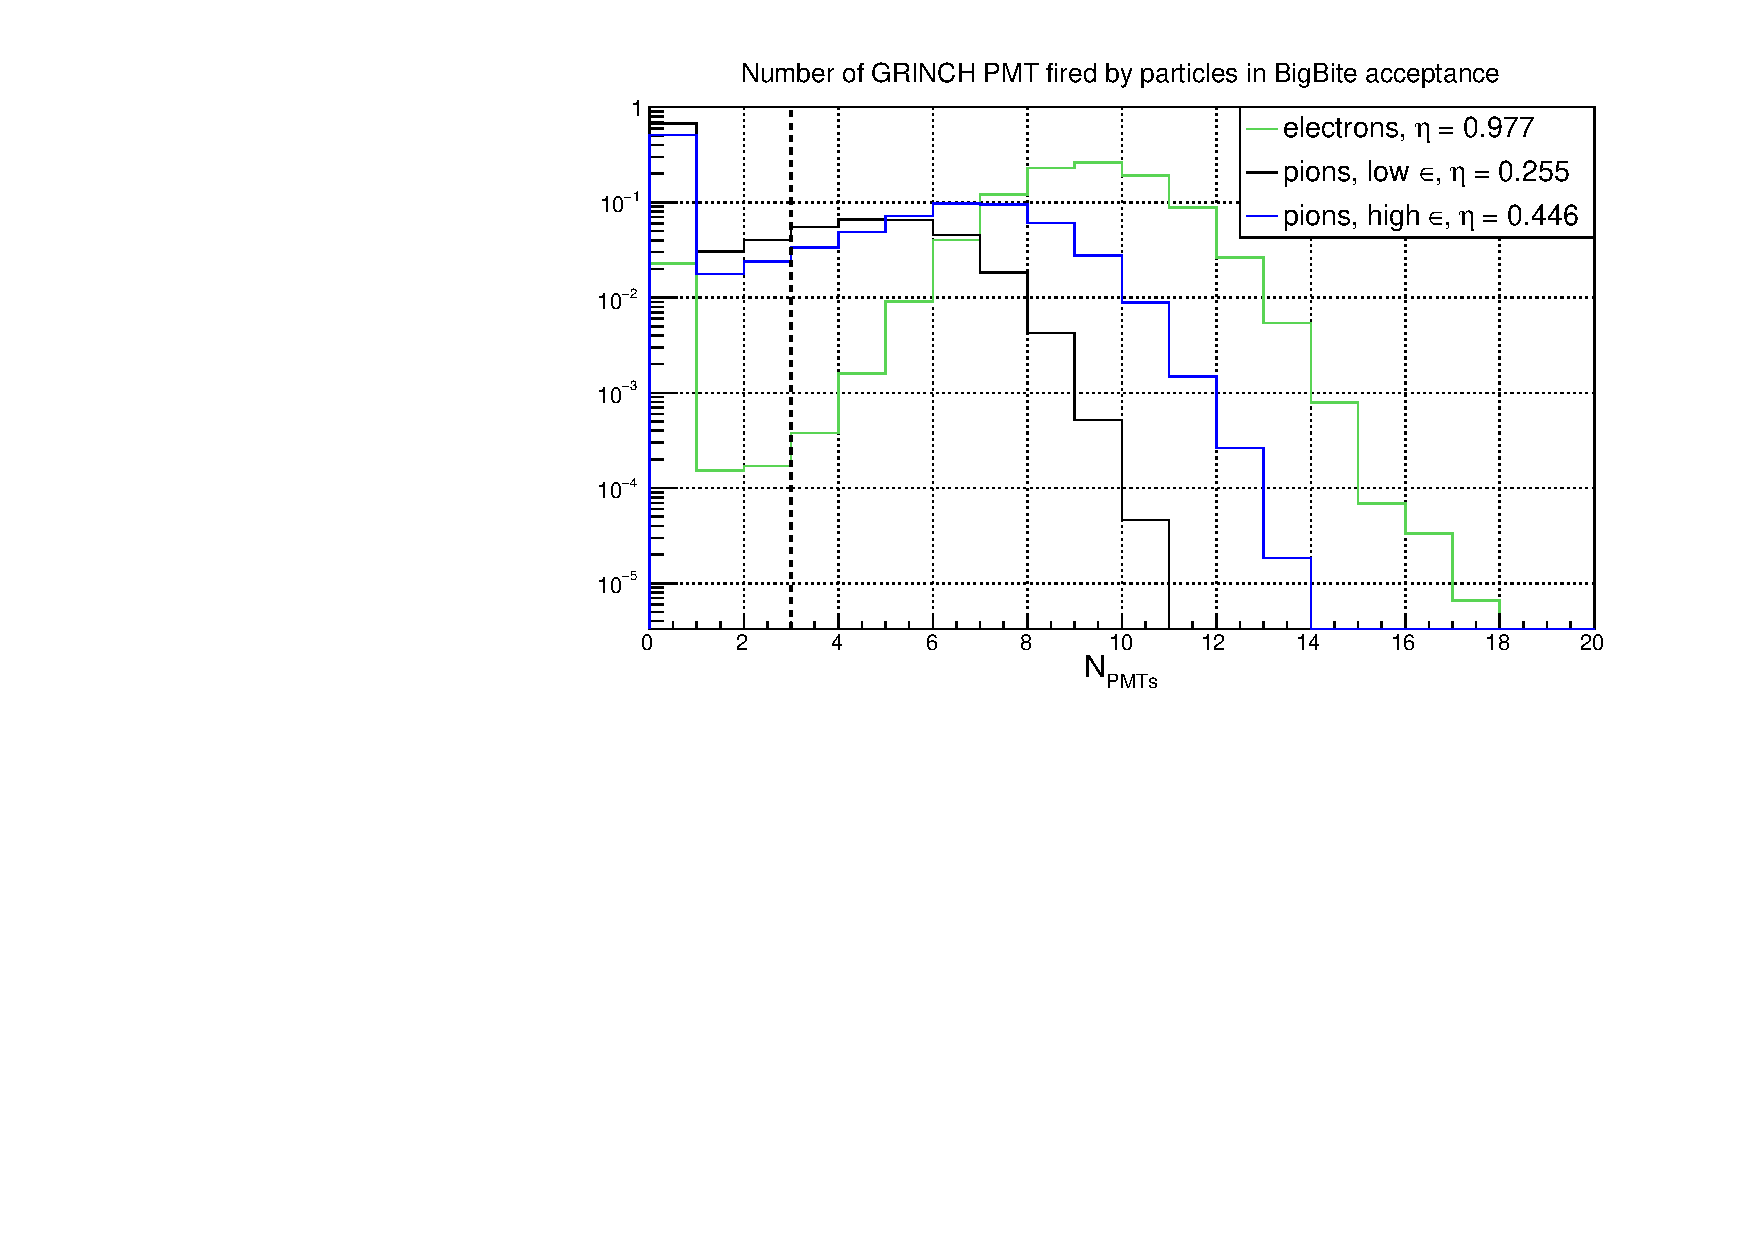
\includegraphics[width=6cm]{Plots/GRINCH_rejection.pdf}
%    \caption{GRINCH response for electrons (green), pions at the low $\epsilon$ kinematic ($k' = 2.0$)}
%    \label{fig:GRINCH_rej}
%  \end{center}
%\end{figure}
%



%For $12~\mathrm{GeV}$ running, to provide a pion threshold of $3.5~\mathrm{GeV}$, a combination of about $50\%$ $\mathrm{CO}_2$, $50\%$ Freon-12 will be used.

%For our conditions, the rate of electrons will be about $30~\mathrm{kHz}$, which in a $100~\mathrm{ns}$ gate will lead to a $0.3\%$ chance of a pion being misidentified by an accidental electron.  
%Using standard calculations, for a charged pion near threshold, there is a $0.1\%$ chance of producing a $\delta$ electron above threshold.  
%Combined, a pion rejection factor from the Cerenkov will be about 1:250, near specifications.  
%Combined with a rejection factor of 1:50 for the preshower provides a $10^4$ overall rejection.

%v4.4
\subsection{Hadron Calorimeter (HCal)}
%
\label{sec:expsetup_hcal}

The Hadron Calorimeter (HCal) has been designed specifically to measure the recoil nucleon for the SBS experiments. Specifically for this experiment (and for $G_M^n$), HCal combined with the SBS (48D48) magnet provides identification of the recoil nucleon, as well as additional kinematic constraint and possibly timing information on the measured interaction.
Nucleon identification is illustrated on Fig.~\ref{fig:hcal_nuclimprint}. This figure shows the compared proton and neutron position distribution in HCal at the same electron kinematics. The proton distribution is being shifted upwards by about $1~\mathrm{m}$ compared to the neutron.
%
\begin{figure}[!h]
  \begin{center}
    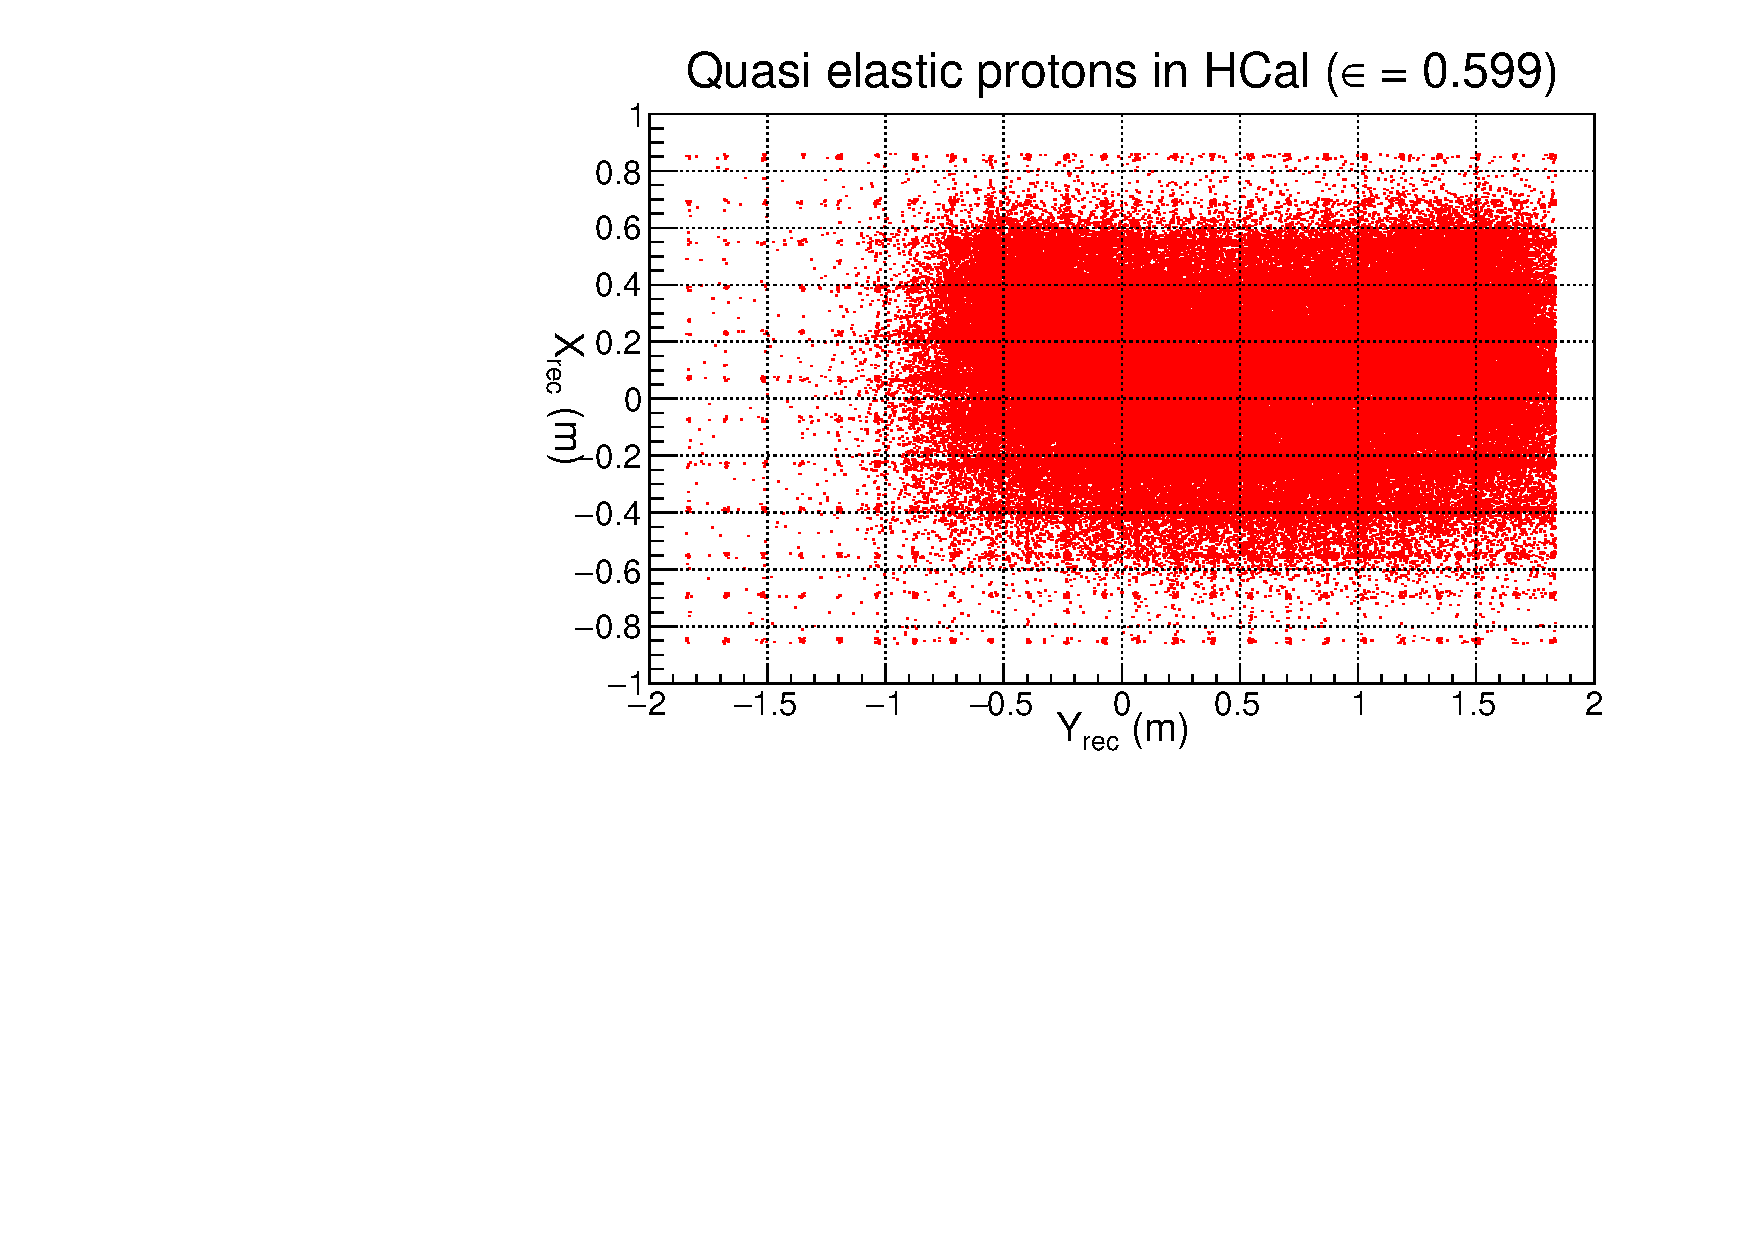
\includegraphics[angle=90,width=4cm]{Plots/HCal_p.pdf}
    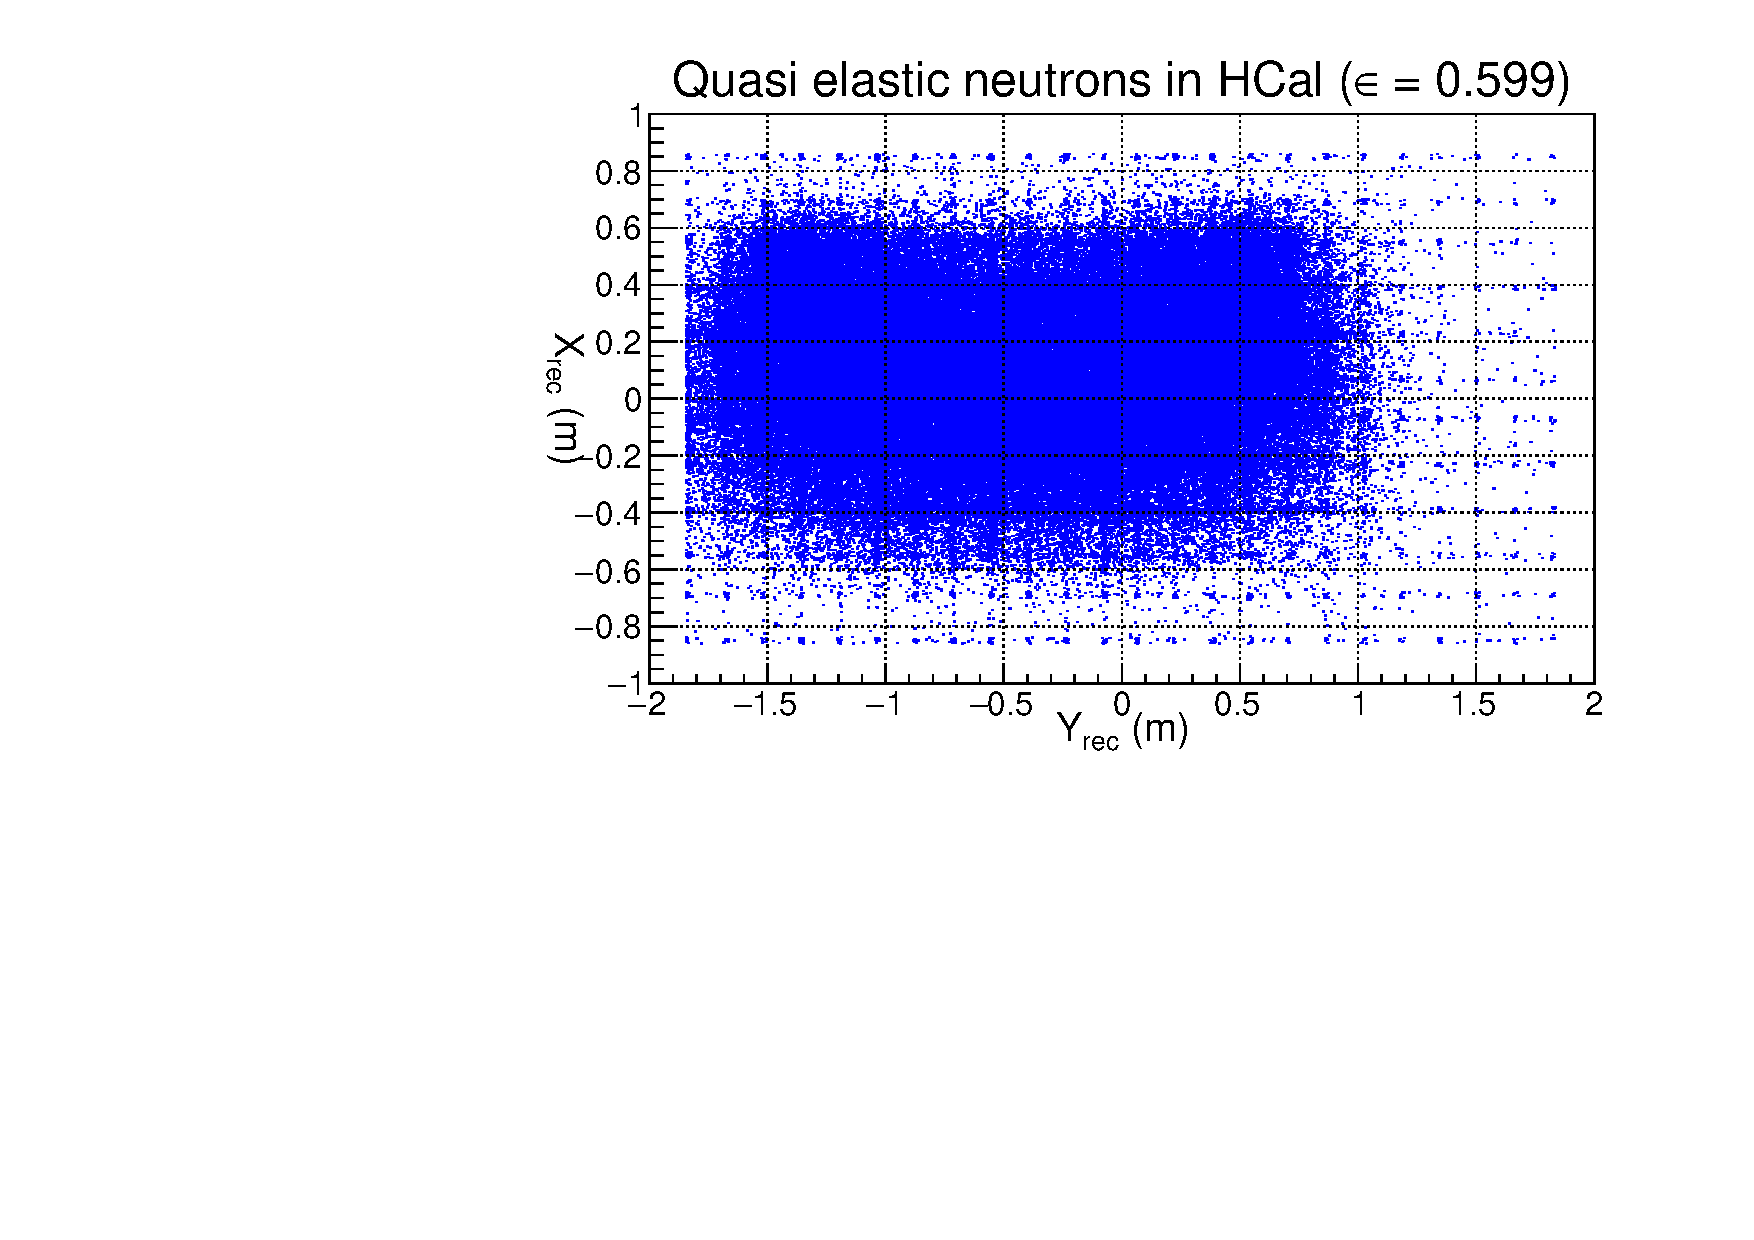
\includegraphics[angle=90,width=4cm]{Plots/HCal_n.pdf}
    \caption{Reconstructed HCal cluster from quasi-elastic events generated by G4SBS. The left distribution in red is for the proton, the right distribution in blue is for the neutron.}
    \label{fig:hcal_nuclimprint}
  \end{center}
\end{figure}
%

%\subsubsection{Structure of the HCal}

The HCal (which CAD model is shown on Fig.~\ref{fig:hcal_cad}) is composed of 288 modules arranged in an array of $12\, \times \, 24$
%
\begin{figure}[!h]
  \begin{center}
    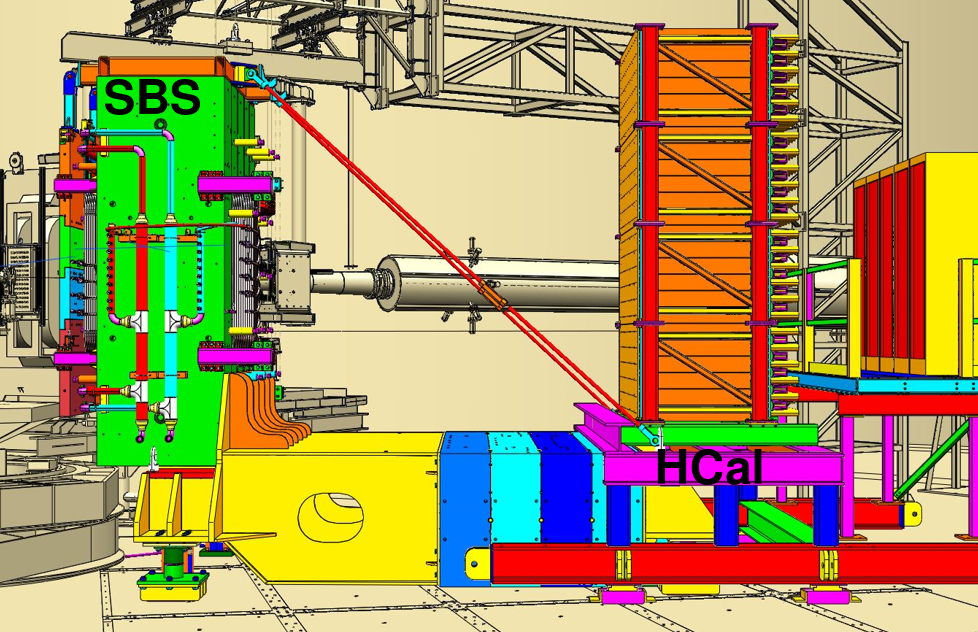
\includegraphics[width=10cm]{Plots/Wines_SBS_CAD_Fall2018.png}
    \caption{CAD representation of HCal (right) with the SBS magnet (left)}
    \label{fig:hcal_cad}
  \end{center}
\end{figure}
%
In front of the full assembly is located a $3/4~\mathrm{in}$ steel plate which purpose is double:
%
\begin{itemize}
\item{initiate the hadronic shower to optimize the calorimeter response;}
\item{shield the modules from a fraction of the low energy secondaries;}
\end{itemize}
%
Each of these modules measures $6\,\times~6\,\mathrm{in}^2$ section, for $3~\mathrm{ft}$ length. They are composed of alternating tiles of scintillators and iron around a central light guide which collects the light generated in the scintillators by the hadronic shower, and guides it to the PMT at the end of the block.
Cosmics tests have determined that the average light yield for the HCal modules is around 5 photoelectrons per MeV deposited in the scintillator tiles.

The PMTs are readout with FAD250 which sample the PMT signal every 40 ns and allow to reconstruct the PMT pulse shape, hence its timing.
They are also readout by TDCs which provide additional timing information.
Thanks to this, the timing resolution can be better than $1~\mathrm{ns}$, which cosmics tests (in progress) seem to confirm.

The energy resolution is intrinsically broad (see Fig.~\ref{fig:HCalRates} in Section~\ref{sec:simu}), due mostly to the small fraction of energy from the hadronic shower actually measured by the scintillator tiles ($\leq 0.1$ - refer yet again to Fig.~\ref{fig:HCalRates}).

%Note that the photoelectron statistics in the PMTs should not be a huge contributor to the resolution width. 
%\subsubsection{Parameters of the HCal}
\iffalse
The HCal angle and distance to the target will move from a kinematic to the other. At 8.5 m which is the largest distance for this experiment, the solid angle from the target is about 90 msr.
The matching between the electron in BigBite and the nucleon in HCal is about 90\% for the low $\epsilon$ kinematic.
For the high $\epsilon$ kinematic, HCal has to be brought closer to the target because the nucleon imprint is larger (Fig.~\ref{fig:hcal_nuclimprint2}).
%\iffalse
%
\begin{figure}[!h]
  \begin{center}
    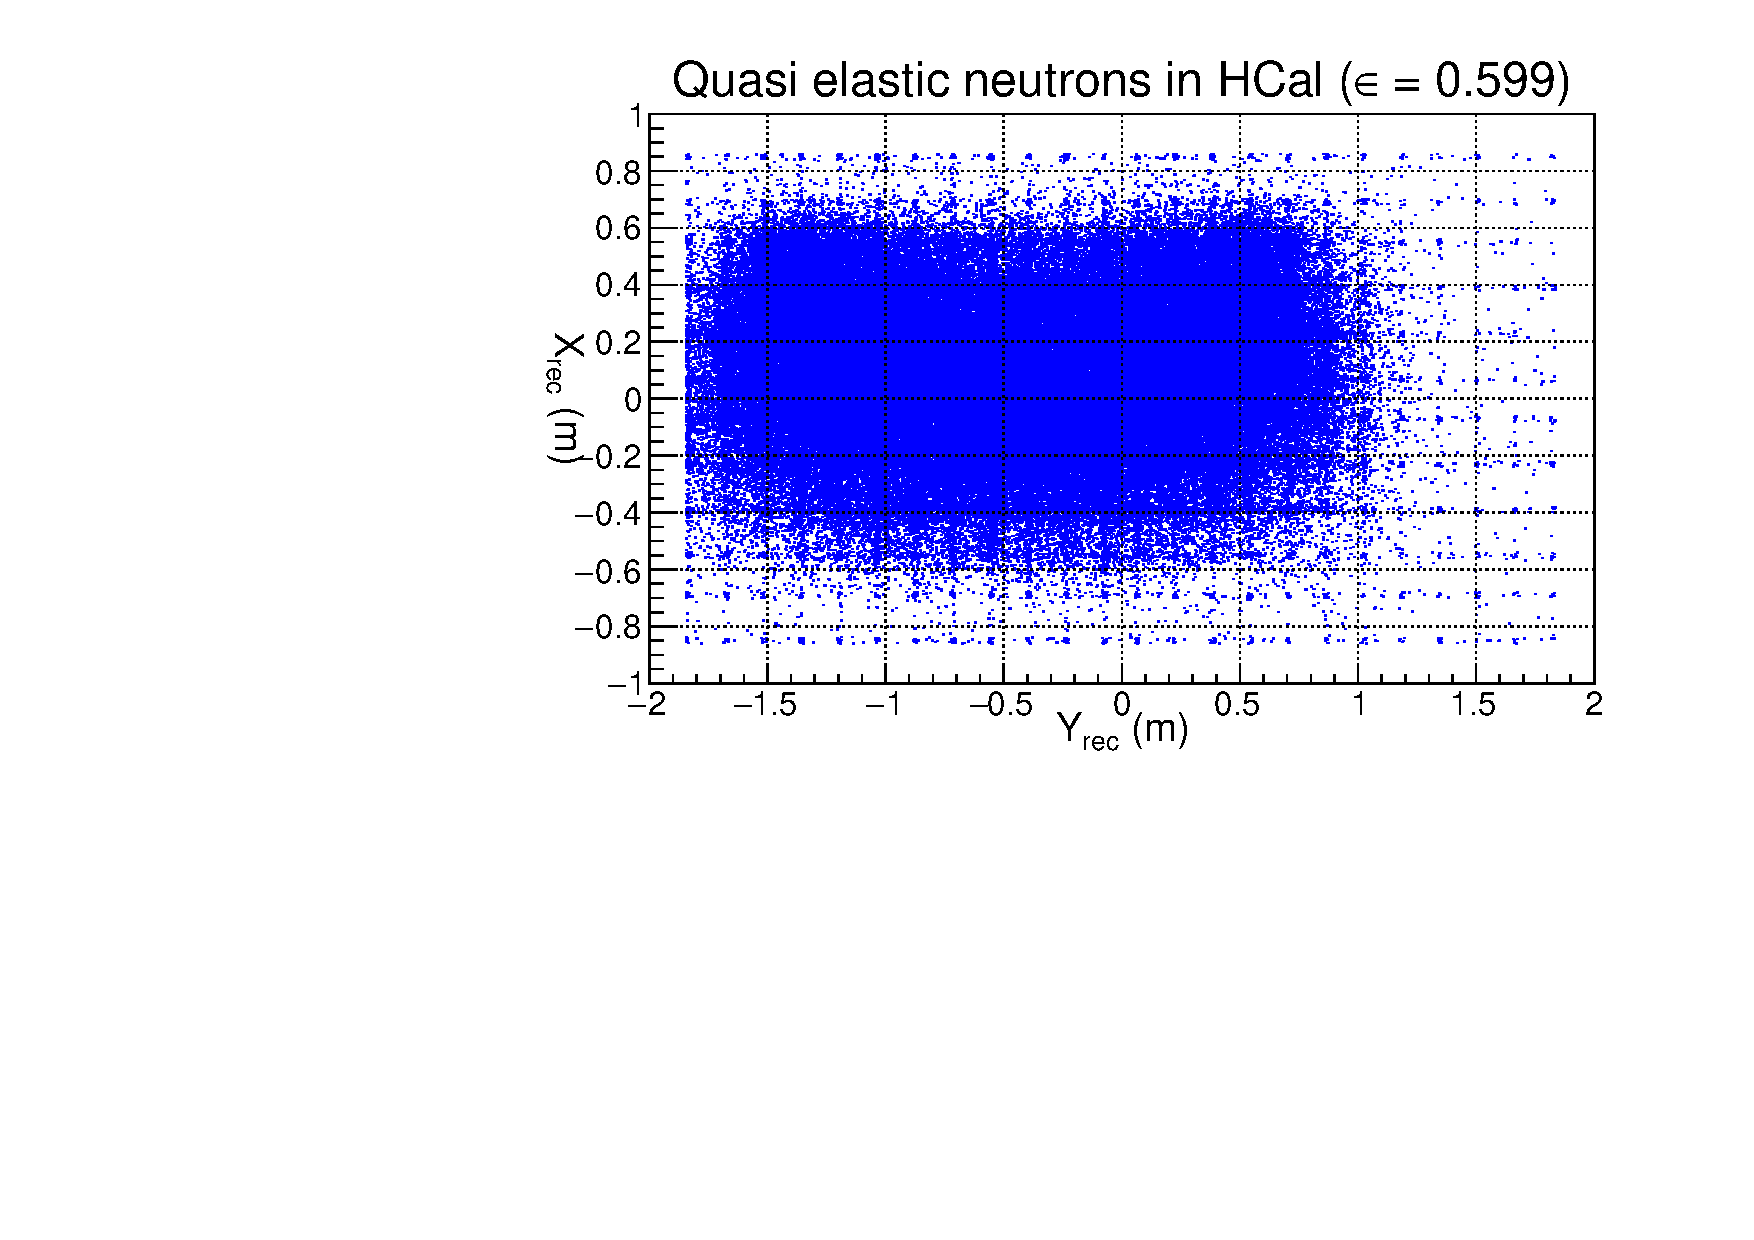
\includegraphics[angle=90,width=4cm]{Plots/HCal_n.pdf}
    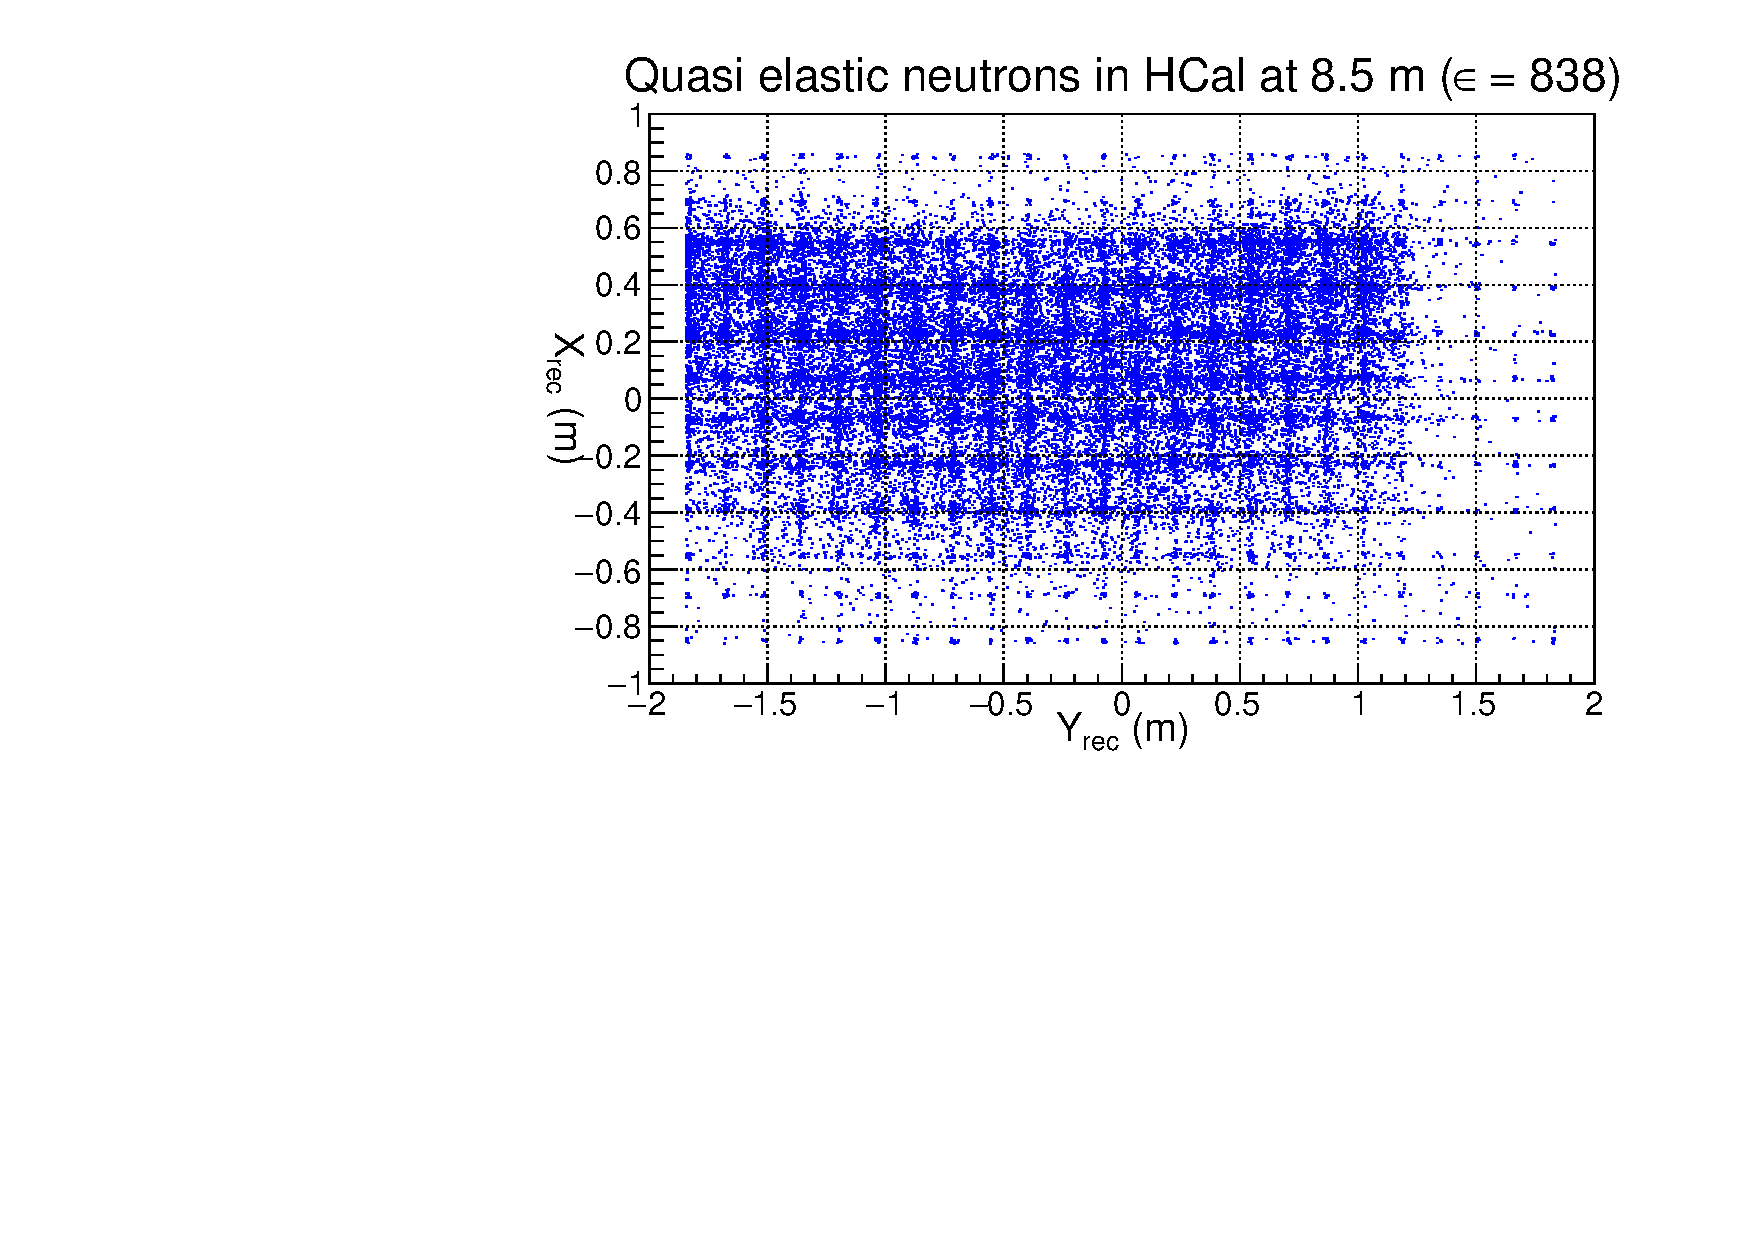
\includegraphics[angle=90,width=4cm]{Plots/HCal_n_he.pdf}
    \caption{Reconstructed HCal cluster from quasi-elastic events generated by G4SBS. The left distribution is for the neutron at the low $\epsilon$ kinematic, the right distribution is for the neutron at the high $\epsilon$ kinematic, and the same distance from the target.}
    \label{fig:hcal_nuclimprint2}
  \end{center}
\end{figure}
%
\fi


%
\section{Simulations, estimations of counting rates and accidentals}
\label{sec:simu}

The estimations of counting rates accidentals have been performed using G4SBS, the GEANT4-based simulation package developed for the SBS experiment \cite{g4sbs}.
This package includes a wide range of event generators, which allows to evaluate the rates for both events of interest (signal) and background.
%, such as elastic/quasi-elastic.
The representation of the experiment apparatus in G4SBS is shown in the high $\epsilon$ configuration on Fig.~\ref{fig:g4sbssetup}. 
%This model includes many details about the beamline, scattering chamber, and all other elements 
%
\begin{figure}[!h]
  \begin{center}
    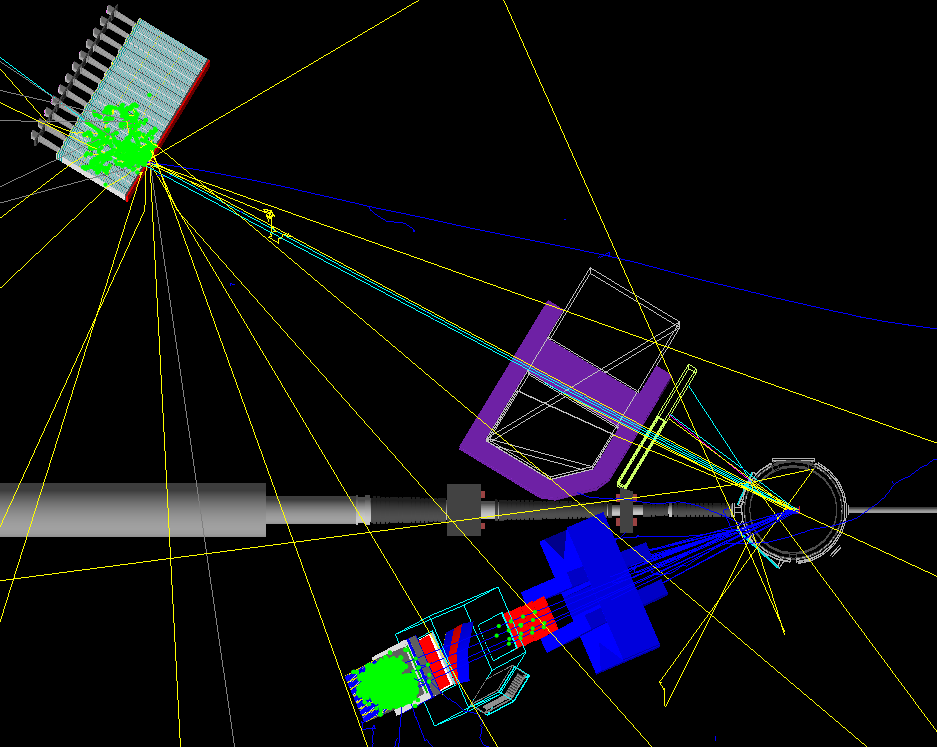
\includegraphics[width=9.6cm,height=8cm]{Plots/SetupHiEPoint.png}
    \caption{Top view of the experimental apparatus model in G4SBS, shown in the high $\epsilon$ configuration. The beam direction is indicated, as well as the main elements (HCal, SBS magnet, BigBite spectrometer)}
    \label{fig:g4sbssetup}
  \end{center}
\end{figure}
%
%Most of the subsystems are mostly accurately reproduced in G4SBS, using the correct 

\subsection{Background and trigger rates}

The main processes expected to contribute the trigger rates for the BigBite spectrometer are:
%
\begin{itemize}
\item{the inelastic electron nucleon scattering process;}
\item{photons from inclusive $\pi^0$ production;}
\item{and to a lesser extent, charged pions.}
\end{itemize}
%
One the other hand, we expect all sorts of hadronic backgrounds to contribute to the rates in HCal, the dominant ones being pions.
Both the inelastic scattering and the inclusive neutral and charged pion production are implemented in G4SBS, the latter relying on the Wiser parametrization \cite{wiser}.
We may also considered the minimum-bias ``beam-on-target'' generator for the HCal background, especially at lower angle (all electromagnetic and hadronic processes being built-in in G4SBS).

The thresholds to apply to each arm are determined as a function of the elastic peak.
For the electron arm, the threshold has been set at $\mu_E - 2.5 \sigma_E$,  $\mu_E$ and $\sigma_E$ being respectively the position and width of the fitted elastic peak. 
Fig.~\ref{fig:BBRates} presents the distributions of rate of energy deposit for the different processes involved in the BigBite trigger rates. 
%
\begin{figure}[!h]
  \begin{center}
    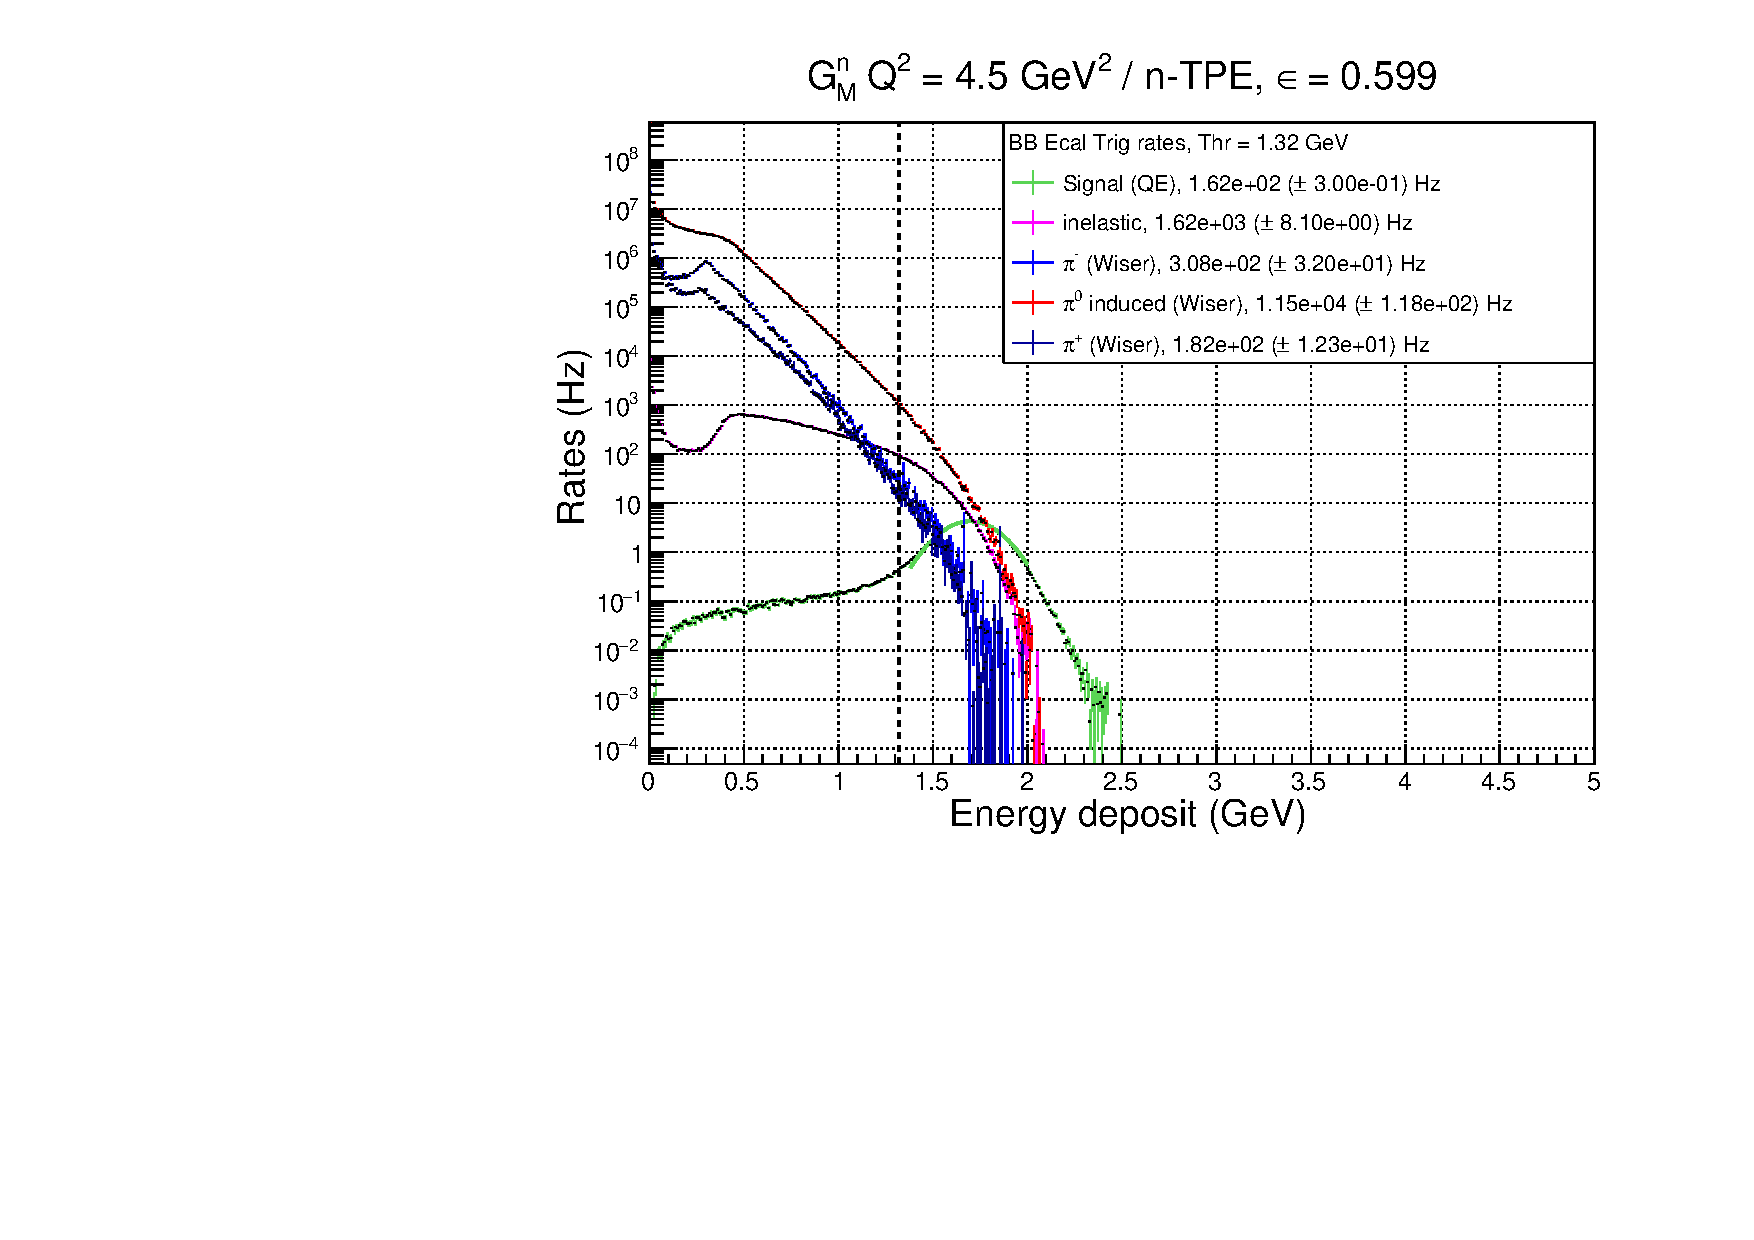
\includegraphics[width=6cm]{Plots/BBECalRates_gen-tpe_le.pdf}
    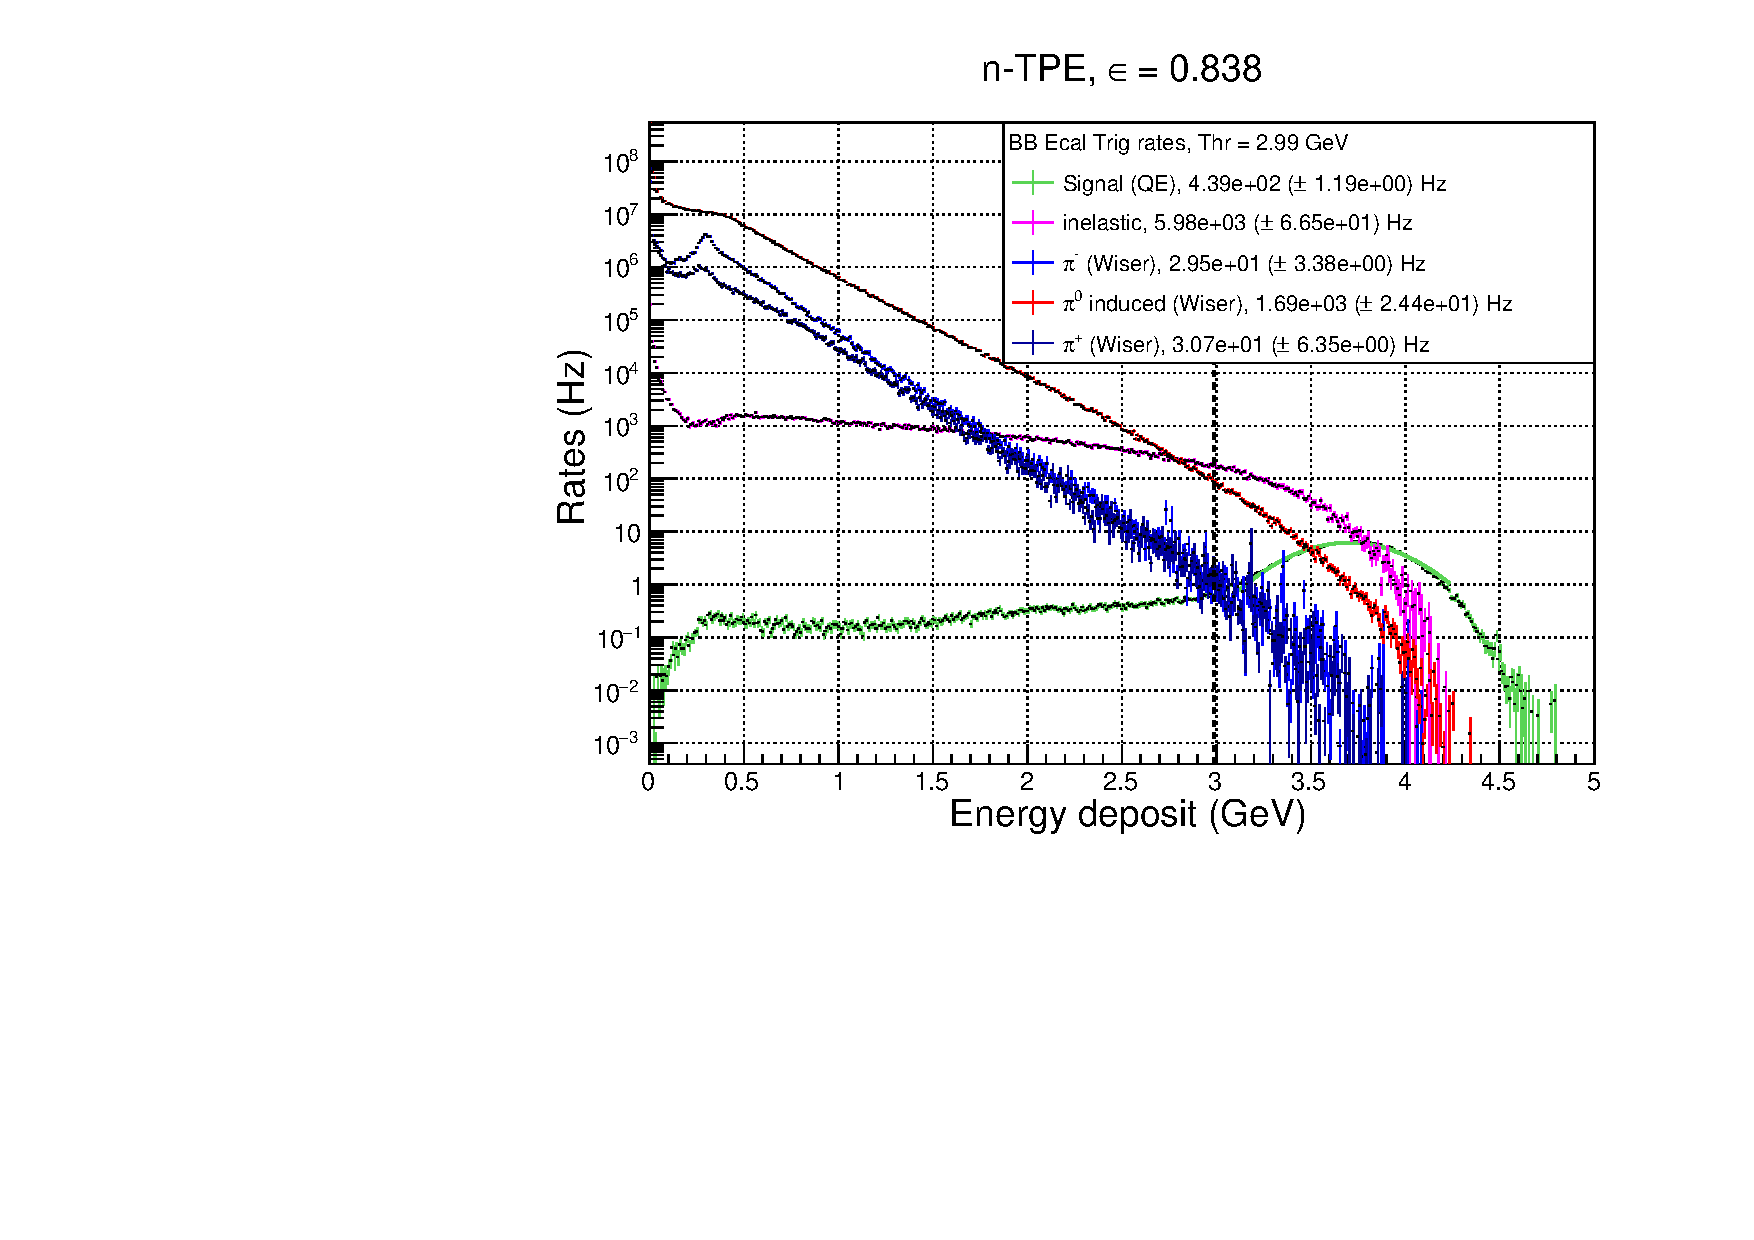
\includegraphics[width=6cm]{Plots/BBECalRates_gen-tpe_he.pdf}
    \caption{Rates of the different process contributing to the BigBite electron arm trigger, for the low $\epsilon$ (left) and the high $\epsilon$ (right). Quasi-elastic is in green, inelastic in magenta, $\pi0$ in red, $\pi^-$ in blue, and $\pi^+$ in dark blue. Note the resolution for the elastic peak in the BigBite shower is $\sim0.3$ GeV.}
    \label{fig:BBRates}
  \end{center}
\end{figure}
%

Since HCal is a sampling calorimeter (meaning that only a fraction of the shower energy is measured), it's resolution is significantly wider ($\sim0.7$ GeV).
Due to this, the threshold is at 90\% efficiency (which corresponds to $\sim$0.1 GeV for both kinematics.
Fig.~\ref{fig:HCalRates} presents the distributions of rate of energy deposit for the different processes involved in the BigBite trigger rates.
%
\begin{figure}[!h]
  \begin{center}
    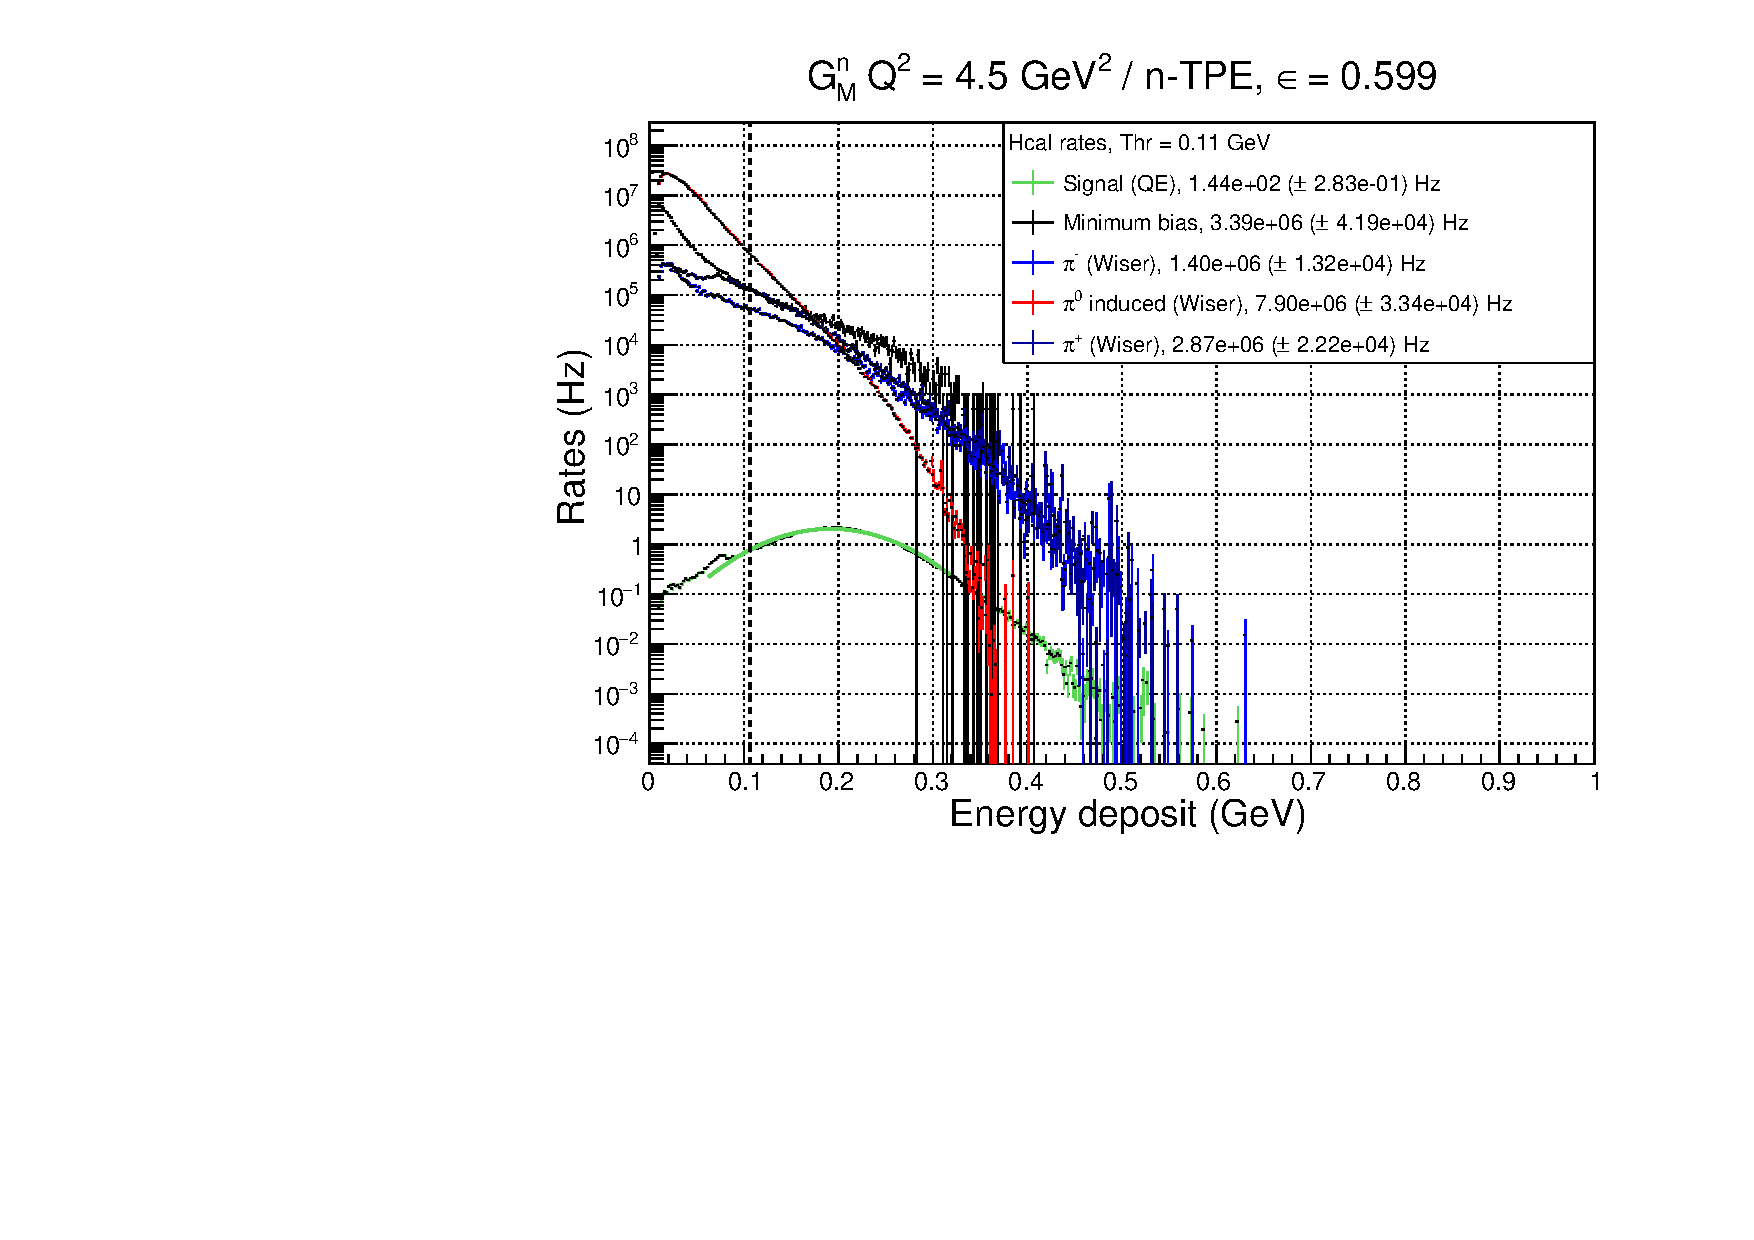
\includegraphics[width=6cm]{Plots/HCalRates_gen-tpe_le.pdf}
    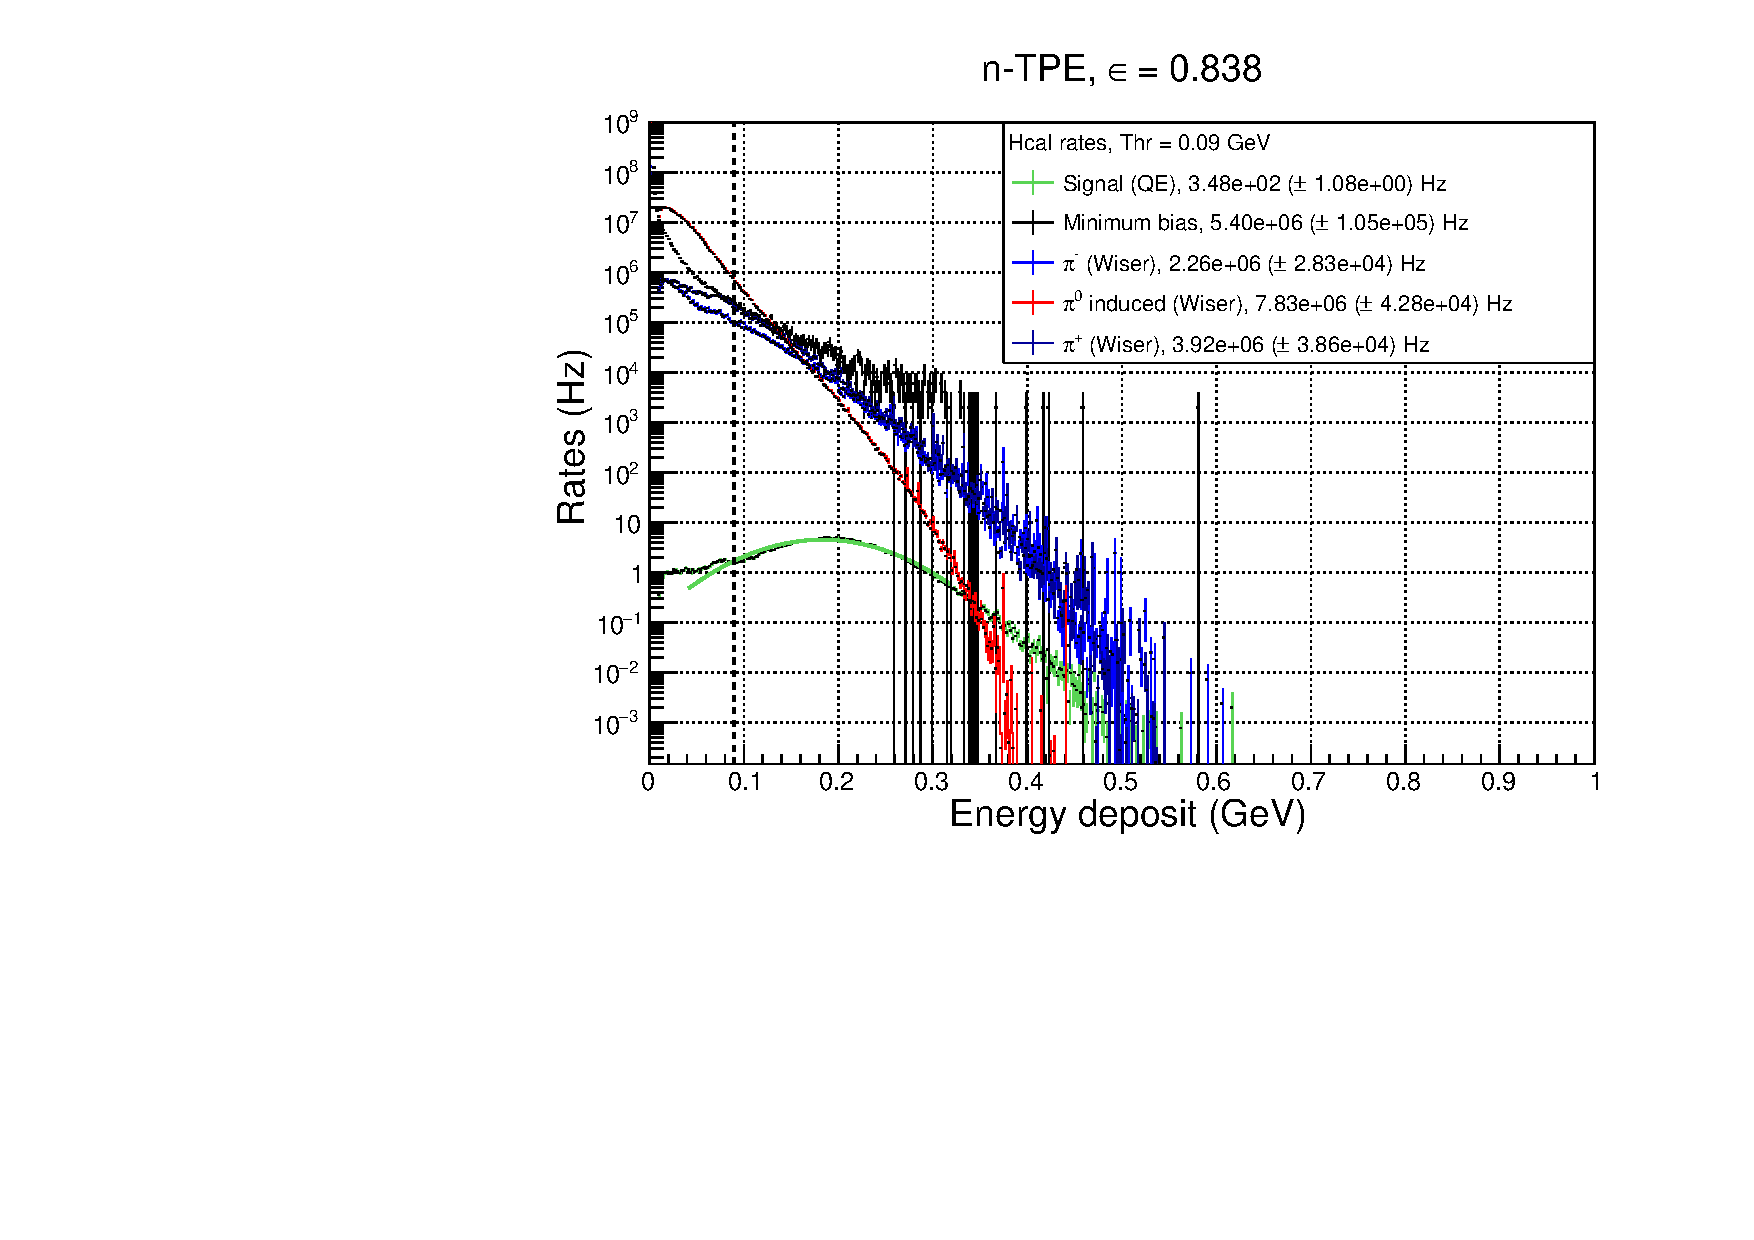
\includegraphics[width=6cm]{Plots/HCalRates_gen-tpe_he.pdf}
    \caption{Rates of the different process contributing to the HCal trigger, for the low $\epsilon$ (left) and the high $\epsilon$ (right). Quasi-elastic is in green, minimum bias in black, $\pi0$ in red, $\pi^-$ in blue, and $\pi^+$ in dark blue. Note the peak itself is around 0.2 GeV for 3.2 GeV nucleons.}
    \label{fig:HCalRates}
  \end{center}
\end{figure}
%

The thresholds and trigger rates for each arm, as well as the coincidence rate (assuming 30ns coincidence window), are summarized in Table.~\ref{tab:TrigRates}.
%
\begin{center}
\begin{table}[h]
\begin{tabular}{|l|c|c|c|c|}
\hline
Point ($\epsilon$) & \multicolumn{2}{|c|}{1 (0.599)} & \multicolumn{2}{c|}{2 (0.838)} \\
\hline
& BigBite & HCal & BigBite & HCal \\ 
& rates (Hz) & rates (Hz) & rates (Hz) & rates (Hz) \\
\hline
threshold (GeV) & 1.32 & 0.106 & 2.99 & 0.090 \\
\hline
Quasi-elastic   & 1.62$\times 10^{2}$ & 1.44$\times 10^{2}$ & 4.39$\times 10^{2}$ & 3.48$\times 10^{2}$ \\
Inelastic       & 1.62$\times 10^{3}$ & - & 5.98$\times 10^{3}$ & - \\
$\pi^-$ (Wiser) & 3.08$\times 10^{2}$ & 1.40$\times 10^{6}$ & 2.95$\times 10^{2}$ & 1.96$\times 10^{6}$ \\
$\pi^0$ (Wiser) & 1.15$\times 10^{4}$ & 7.90$\times 10^{6}$ & 1.69$\times 10^{3}$ & 5.77$\times 10^{6}$ \\
$\pi^+$ (Wiser) & 1.82$\times 10^{2}$ & 2.87$\times 10^{6}$ & 3.07$\times 10^{2}$ & 3.34$\times 10^{6}$ \\
Minimum bias    & - & 3.39$\times 10^{6}$ & - & 3.32$\times 10^{6}$($^*$) \\ 
\hline
{\em Total} & 1.37$\times 10^{4}$ & 1.22$\times 10^{7}$ & 8.17 $\times 10^{3}$ & 1.11$\times 10^{7}$ \\
(min. bias - HCal only) &  & / 3.39$\times 10^{6}$ &  & / 3.32$\times 10^{6}$ \\
\hline
{\bf Coincidence rate} & \multicolumn{2}{|c|}{5.01$\times 10^{3}$} & \multicolumn{2}{c|}{2.72$\times 10^{3}$} \\
(with min. bias HCal) & \multicolumn{2}{|c|}{1.39$\times 10^{3}$} & \multicolumn{2}{|c|}{8.14$\times 10^{2}$} \\
\hline
\end{tabular} 
\caption{Trigger rates for BigBite and HCal, with the different process contributions separated, and the sum. For HCal, the total rates is either the sum of the (Wiser) inclusive pions or the minimum bias. The coincidence rates assume a 30 ns coincidence window.}
\label{tab:TrigRates}
\end{table}
\end{center}
%
Note that for HCal, the ``total rates'' is either the sum of inclusive charged and neutral pions evaluated with the Wiser cross sections {\em or} the ``minimum bias'' beam on target. We have good reasons to think that the Wiser code results actually overestimate the HCal rates, but for the sake of thoroughness, we have checked the coincidence rates assuming the sum of the inclusive pions (evaluated with the Wiser cross sections) as the HCal rates.

In the worst case scenario, the coincidence rates could be as high as 5kHz, which might be at the limit of manageability for the DAQ.
However, a slight increase on the HCal threshold (which would drop the efficiency from $\sim$90\% to $\sim$85\%) would decrease the total HCal rates by $\sim$35\% to 40\% in this worst case scenario, which would make the situation more manageable (3.3 kHz).

\subsection{Accidentals: contamination from inelastic}

The main source of contamination for the quasi-elastic comes from the inelastic electron-nucleon scattering. Most of this contamination can be cleaned out thanks to a selection on the center of mass energy
%
\begin{equation}
  W^2 = M_{N}^2+2M_{N}^{2}(E-E')-Q^2, %= (q+p)^2 
\end{equation}
%
and the missing transverse momentum of the nucleon
%
\begin{equation}
  p_{\perp miss} = \sqrt{(q_{x}-p'_{x})^2+(q_{y}-p'_{y})^2},
\end{equation}
%
where $M_N$ is the mass of the nucleon, $E$ and $E'$ the initial and final energy of the electron, and $q_{x,y}$, $p'_{x, y}$ are the projections on $x$, $y$ of the vectors of the virtual photon and final nucleon.
The distributions of these quantities (weighted with cross section and including detector resolutions) are displayed for quasi-elastic and inelastic scattering, and for proton and nucleon, on Fig.~\ref{fig:inel_contam_le} for the low $\epsilon$ kinematic, and on Fig.~\ref{fig:inel_contam_he} for the high $\epsilon$ kinematic.
%
\begin{figure}[!h]
  \begin{center}
    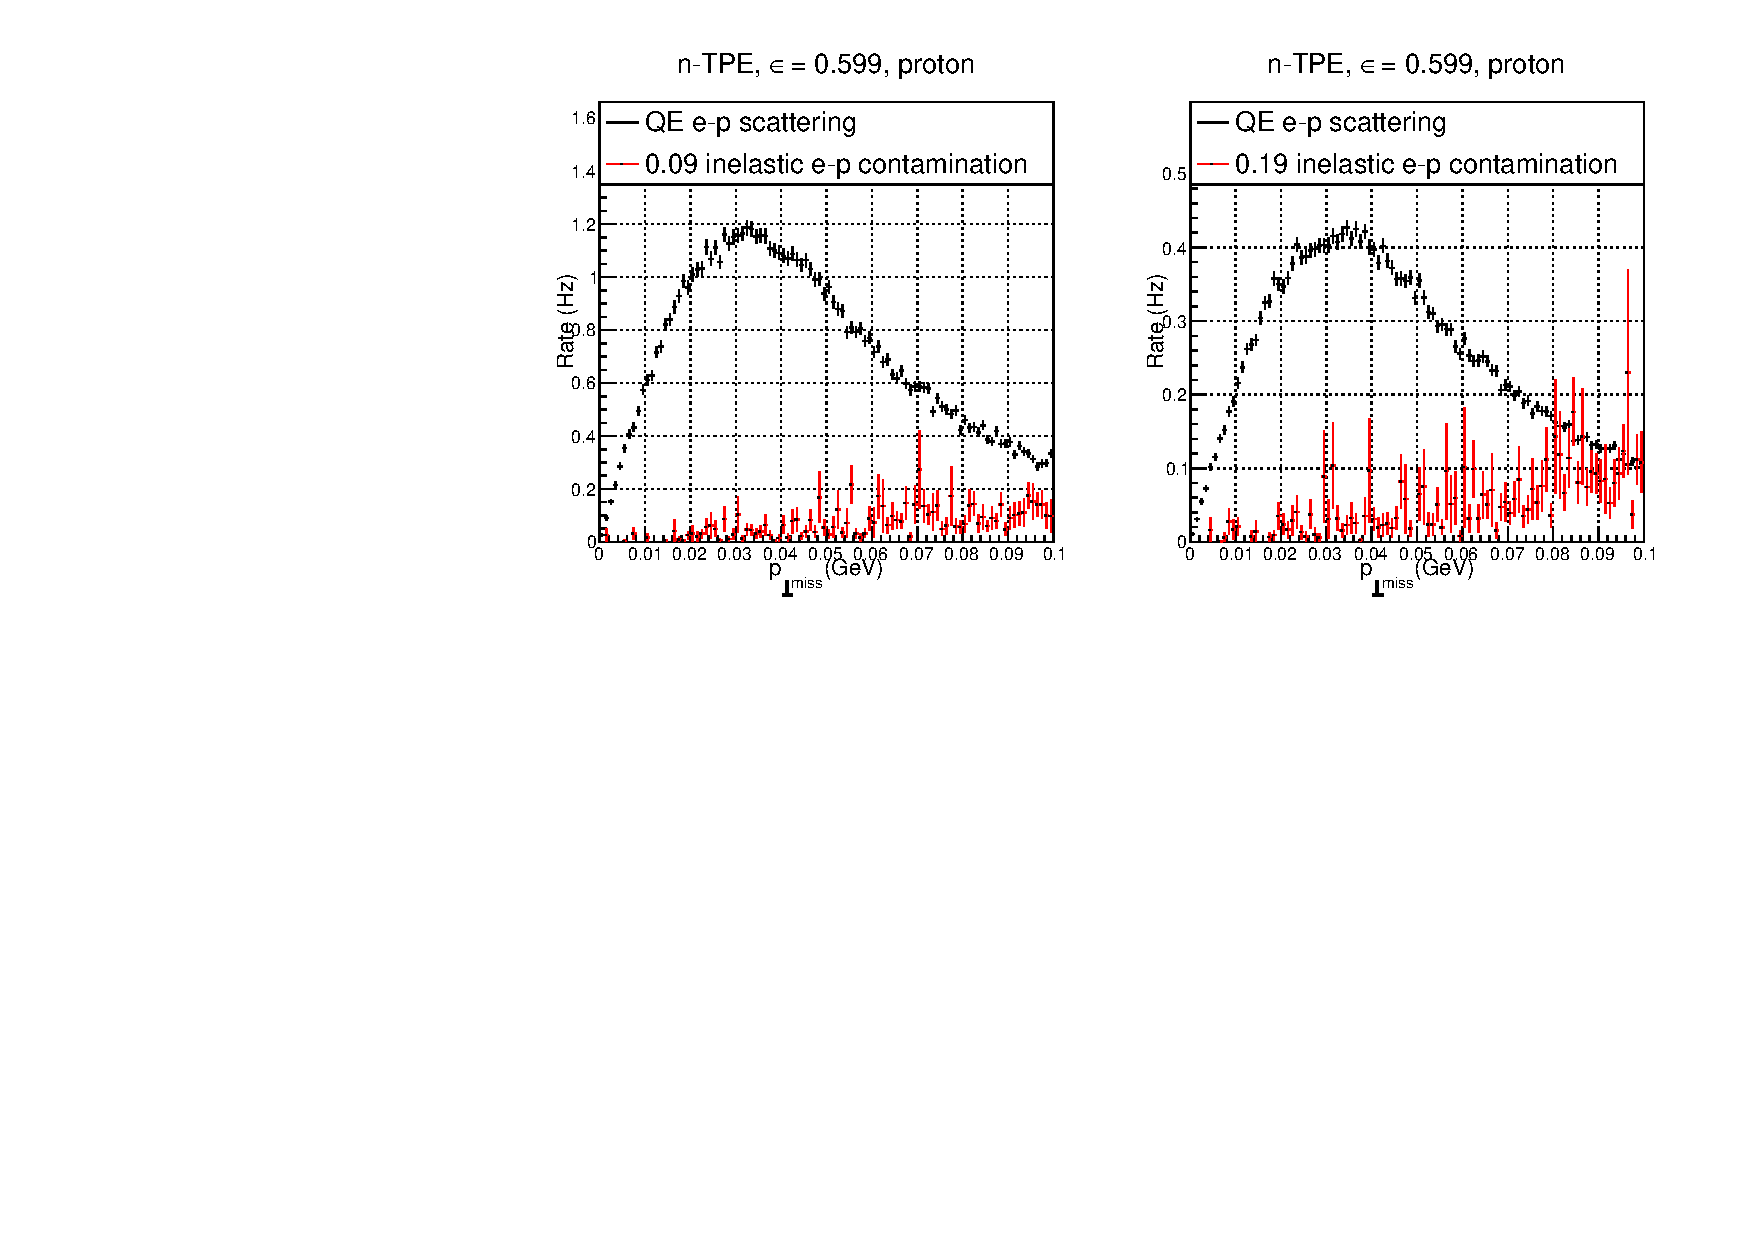
\includegraphics[width=12cm]{Plots/gen-tpe_le_pperp_acc.pdf}
    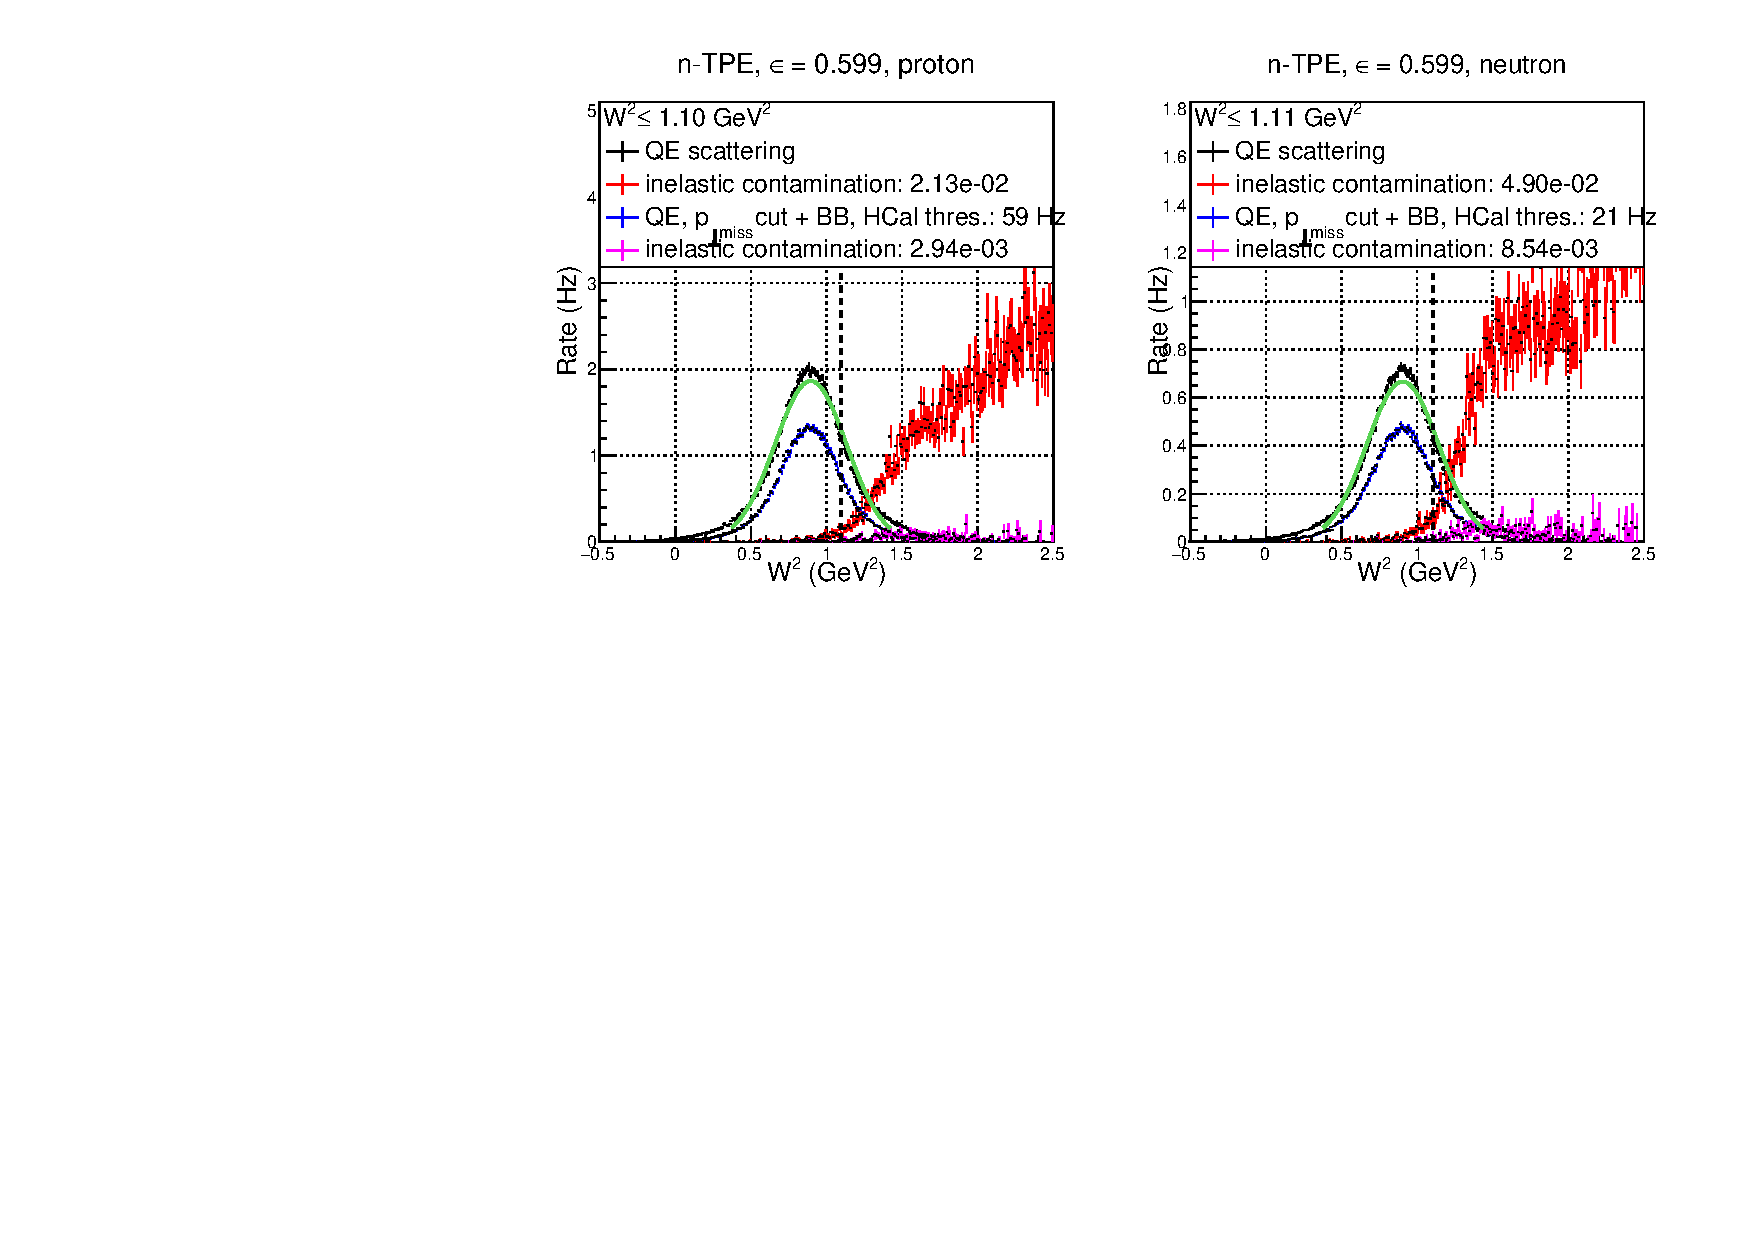
\includegraphics[width=12cm]{Plots/gen-tpe_le_W2_acc.pdf}
    \caption{Compared quasi-elastic and inelastic distributions (including detectors resolutions) for $p_{\perp miss}$ (top) and $W^2$ (bottom), for the low $\epsilon$ kinematic. Comparison for protons is on the left, and comparison for neutrons is on the right. On the bottom panel, black and red are before the $p_{\perp miss}~\leq~0.1~\mathrm{GeV}$ selection, while blue and magenta are after $p_{\perp miss}~\leq~0.1~\mathrm{GeV}$ selection and application of BigBite shower and HCal thresholds.}
    \label{fig:inel_contam_le}
  \end{center}
\end{figure}
%
\begin{figure}[!h]
  \begin{center}
    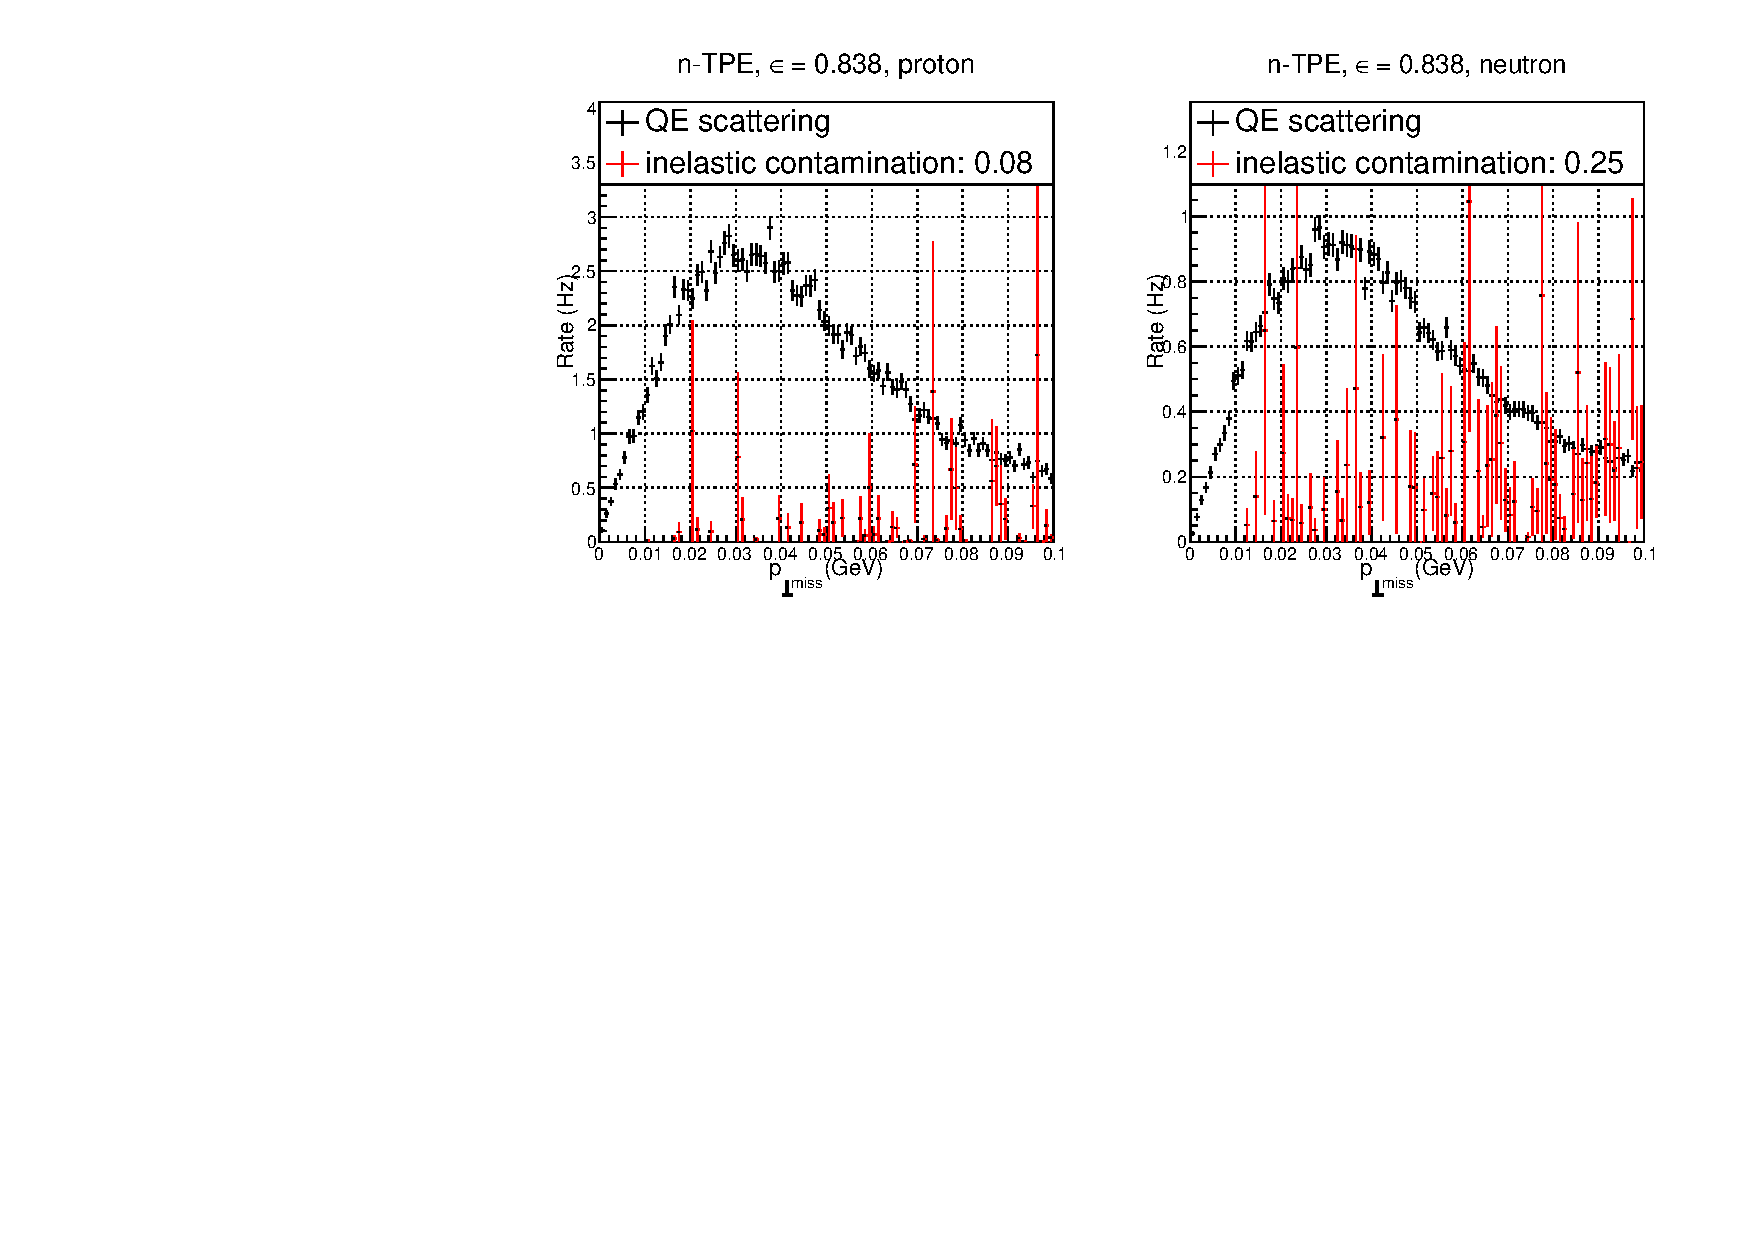
\includegraphics[width=12cm]{Plots/gen-tpe_he_pperp_acc.pdf}
    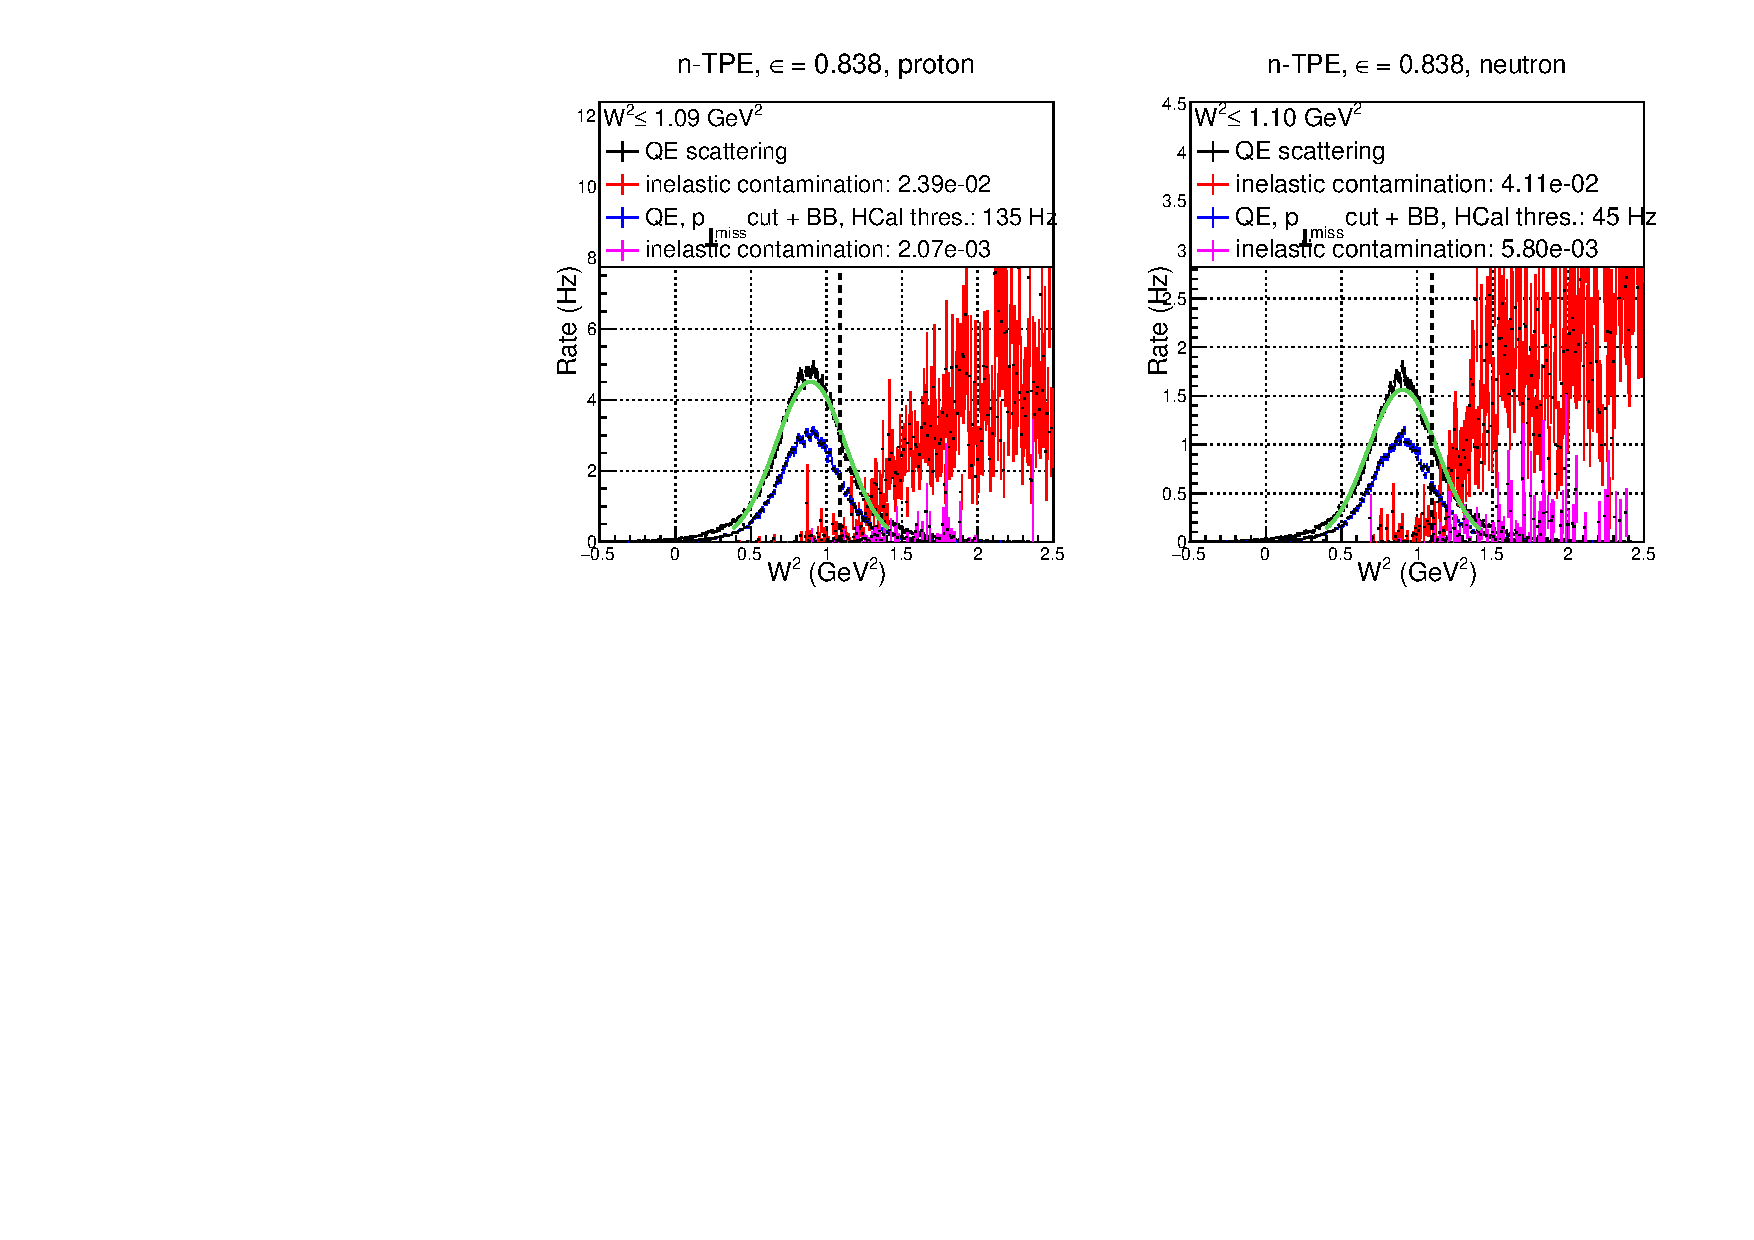
\includegraphics[width=12cm]{Plots/gen-tpe_he_W2_acc.pdf}
    \caption{Compared quasi-elastic and inelastic distributions (including detectors resolutions) for $p_{\perp miss}$ (top) and $W^2$ (bottom), for the high $\epsilon$ kinematic. Comparison for protons is on the left, and comparison for neutrons is on the right. On the bottom panel, black and red are before the $p_{\perp miss}~\leq~0.1~\mathrm{GeV}$ selection, while blue and magenta are after $p_{\perp miss}~\leq~0.1~\mathrm{GeV}$ selection and application of BigBite shower and HCal thresholds.}
    \label{fig:inel_contam_he}
  \end{center}
\end{figure}
%
Provided that we are not limited by statistics and the sample purity is capital for our experiment, we set the selection criteria on $W^2$ and $p_{\perp miss}$ to maximize inelastic contamination (ideally below 1~\%). 
Setting $p_{\perp miss}~\leq~0.1~\mathrm{GeV}$ and $W^2~\leq~1.1~\mathrm{GeV}^2$, the inastic contamination of the elastic sample ranges from 0.2~\% to 0.9~\%, while rataining $\geq$~60~\%. % of statistics listed in Table.~\ref{tab:Rates}

\subsection{Quasi-elastic counting rates}

The signals for this experiment have been generated using the G4SBS elastic/quasi-elastic generator. 
We generated 1M events sample for each kinematics, on a solid angle that was larger than the detector acceptance.
To evaluate the detector solid angle, we define simple criteria that each event has to pass, defined as the following;
%
\begin{itemize}
\item{require a primary track, going through all 5 GEM layers (electron arm);}
\item{require non-zero energy deposit in both the preshower and shower (electron arm);}
\item{require non-zero energy deposit in HCal (hadron arm).}
\end{itemize}
%
The detector solid angle, for both proton and neutron, are defined in Table.~\ref{tab:kinExpParams}
%
\begin{center}
\begin{table}[h]
  %\begin{tabular}{|>{\centering}m{0.3in} |>{\centering}m{0.55in}|>{\centering}m{0.4in}| >{\centering}m{0.4in}| >{\centering}m{0.45in}|>{\centering}m{0.45in}|>{\centering}m{0.4in}|>{\centering}m{0.4in}|>{\centering\arraybackslash}m{0.4in}|}
\begin{tabular}{|c|c|c|c|}
\hline
Point ($\epsilon$) & $\Delta\Omega_e$ & $\Delta\Omega_e \otimes \Delta\Omega_n$ & $\Delta\Omega_e \otimes \Delta\Omega_p$ \\
 & (msr) & (msr) & (msr) \\
\hline
1 (0.599) & 52.4 & 46.7 & 47.2 \\
\hline
2 (0.838) & 32.7 & 20.8 & 22.2 \\
\hline
\end{tabular} 
\caption{Kinematics electron solid angle, and convoluted electron/hadron solid angle}
\label{tab:kinExpParams}
\end{table}
\end{center}
%
Then, we evaluate the detection efficiency. For the electron, we require the energy reconstructed in the BigBite calorimeter to be above a threshold defined as $thr = \mu_E- 2.5* \sigma_E$, as well as a minimum number of GRINCH PMTs fired due to the primary electron; For HCal, we require the threshold to be such as we obtain ~90\% efficiency. These values are summarized in Table.~\ref{tab:kinEffs}.
%
\begin{center}
\begin{table}[h]
\begin{tabular}{|c|c|c|c|c|c|c|c|}
\hline
Point ($\epsilon$) & BB thr. & HCal thr. & $\eta_{det~e}$ & $\eta_{det~n}$ & $\eta_{det~p}$ & $\eta_{sel~n}$ & $\eta_{sel~p}$ \\
 & (GeV) & (GeV) &  &  &  &  &  \\
\hline
1 (0.599) & 1.32 & 0.11 & 0.902 & 0.904 & 0.892 & 0.589 & 0.605 \\ 
\hline
2 (0.838) & 2.99 & 0.09 & 0.808 & 0.889 & 0.882 & 0.617 & 0.647 \\
\hline
\end{tabular} 
\caption{Kinematics electron thresholds, particle detection efficiencies ($\eta_{det}$), and efficiency of quasi-elastic selection $\eta_{sel}$ separated for the proton and the neutron.}
\label{tab:kinEffs}
\end{table}
\end{center}
%

The counting rates are evaluated using the events that have passed the selection described above, and weighting those events with the cross section calculated by G4SBS, multiplied by the generation solid angle, using the formula:
%
\begin{equation}
  N_{est} = {\cal L} \Delta t \times \sum_{i \in accepted~evts} \frac{d\sigma}{d\Omega} *\Delta\Omega_{Gen} /N_{Gen}
\end{equation}
%
Events are ``accepted'' if they meet the following criteria:
%
\begin{itemize}
\item{the electron is in the BigBite acceptance};
\item{the electron passes the BigBite threshold defined in Table~\ref{tab:kinEffs} and gives signal in the GRINCH;}
\item{the nucleon is in the HCal acceptance and passes the HCal threshold defined in Table~\ref{tab:kinEffs};}
\item{the event passes the quasi-elastic selection defined in the previous section {\it i.e.} $W^2~\leq~1.1~\mathrm{GeV}^2$ and $p_{\perp miss}~\leq~0.10~\mathrm{GeV}$.} 
\end{itemize}
%

The counting rates, as well as the reduced cross section $F^2$
and its error $\Delta F^2 = F^2/\sqrt{N_{QE}}$ are compiled for both kinematics in Table.~\ref{tab:Rates}, assuming a running time $\Delta t = 12$~hours of running at a beam intensity of $I_{exp} =~30~\mu$A on a liquid deuterium target with length $l_{tgt}~=~15$~cm and density $d_{tgt}~=~0.169~\mathrm{g.cm}^{-3}$.
%
\begin{center}
\begin{table}[h]
  %\begin{tabular}{|>{\centering}m{0.3in} |>{\centering}m{0.55in}|>{\centering}m{0.4in}| >{\centering}m{0.4in}| >{\centering}m{0.45in}|>{\centering}m{0.45in}|>{\centering}m{0.4in}|>{\centering}m{0.4in}|>{\centering\arraybackslash}m{0.4in}|}
\begin{tabular}{|c|c|c|c|c|c|c|}
\hline
Point ($\epsilon$) & QE $e$-$n$ & QE $e$-$p$ & $F^2_n$ & $\Delta F^2_n$ & $F^2_p$ & $\Delta F^2_p$ \\
 & counts & counts & ($\times 10^{-3}$) & ($\times 10^{-6}$) & ($\times 10^{-3}$) & ($\times 10^{-6}$) \\
\hline
1 (0.599) & 9.07$\times 10^{5}$ & 2.55$\times 10^{6}$ & 0.99 & 1.04 & 2.73 & 1.70 \\
\hline
2 (0.838) & 1.94$\times 10^{6}$ & 5.83$\times 10^{6}$ & 0.72 & 0.52 & 1.93 & 0.80 \\
\hline
\end{tabular} 
\caption{Quasi-elastic counting rates, and ``reduced cross section'' as defined by Eq.~\ref{eq:F2}. These rates assume $\Delta t = 12$~hours of running at a beam intensity of $I_{exp} =~30~\mu$A on a liquid deuterium target with length $l_{tgt}~=~15$~cm and density $d_{tgt}~=~0.169~\mathrm{g.cm}^{-3}$}%({\em preliminary})
\label{tab:Rates}
\end{table}
\end{center}
%

The expression of $F_2$ is: 
%
\begin{equation}
  F^2 = \frac{N_{QE}}{{\cal{L}}_{exp} \cdot \Delta t \cdot  d\sigma_{Mott}/d\Omega  \cdot \Delta\Omega \cdot  \eta}
  \label{eq:F2}
\end{equation}
%
where $\Delta t$ the running time, $\Delta\Omega$ is the convoluted BigBite-HCal solid angle, $\eta$ is the product of all efficiencies (detection efficiencies $\eta_{det}$ $\times$ selection efficiency $\eta_{sel}$)
%($\eta = \eta_{det~e} \times \eta_{det~n/p}  \times \eta_{QE sel~n/p}$)
, and ${\cal{L}}_{exp}$ is the experimental luminosity:
%
\begin{equation}
  {\cal{L}}_{exp} = \frac{I_{exp}}{q_e}*L_{tgt}*d_{tgt}\frac{\cal{N}_A}{m_{D}}.
\end{equation}
%
The calculation of the $F_2$ term requires the evaluation of the Mott cross section
%
\begin{equation}
  \frac{d\sigma_{Mott}}{d\Omega} = (\hbar c\alpha_{EM})^2 \left( \frac{e}{2E} \right)^2 \left( \frac{cos{\theta_e/2}}{sin^2{\theta_e/2}} \right)^2 \frac{E'}{E}
\end{equation}
%
\textcolor{red}{{\it private note}: $\hbar c$ is in $\mathrm{GeV}\cdot\mathrm{cm}^{-1}$, but I've assumed $e=1$.}\\
The Mott cross section has been calculated with the weighted average of the electron variables (momentum and polar angle).
%
\begin{center}
\begin{table}[h]
  %\begin{tabular}{|>{\centering}m{0.3in} |>{\centering}m{0.55in}|>{\centering}m{0.4in}| >{\centering}m{0.4in}| >{\centering}m{0.45in}|>{\centering}m{0.45in}|>{\centering}m{0.4in}|>{\centering}m{0.4in}|>{\centering\arraybackslash}m{0.4in}|}
\begin{tabular}{|c|c|c|c|c|}
\hline
Point ($\epsilon$) & $\langle \theta_e \rangle$ &  $\langle k^{\prime} \rangle$ & $\langle Q^2 \rangle$ & $\sigma_{Mott}$ \\
 & (deg) & (GeV) & (GeV$^2$) & (nb sr$^{-1}$) \\
\hline
1 (0.599) & 41.7 & 2.01 & 4.47 & 6.62 \\ 
\hline
2 (0.838) & 22.9 & 4.26 & 4.40 & 48.0 \\
\hline
\end{tabular} 
\caption{Cross-section weighted average of kinematic variables over the BigBite acceptance. The Mott cross section has been evaluated at these values.}
\label{tab:sigma_mott}
\end{table}
\end{center}
%

\iffalse
The counting rates for the low $\epsilon$ kinematics should be directly comparable to the rates reported in the original $G_M^n$ proposal \cite{gmp}.
In this proposal, the requested running time was 12 hours, with a beam intensity of 10 $\mu$A on a 10 cm long liquid deuterium target with density 0.169~g.cm$^{-3}$.
This luminosity is 4.5 times lower than the currently proposed luminosity.
%
\begin{center}
\begin{table}[h]
\begin{tabular}{|l|c|c|}
\hline
 & $d(e, e'n)p$ & $d(e, e'p)n$ \\
\hline
This estimation & 3.27$\times 10^{4}$ & 9.00$\times 10^{4}$ \\
\hline
Original proposal Table.~8 & 1.20$\times 10^{4}$ & 2.66$\times 10^{4}$ \\ 
\hline
Discrepancy factor & 2.73 & 3.38 \\ 
\hline
\end{tabular} 
\caption{{\em Hourly} rates comparison between these predictions and the original $G_M^n$ proposal, {\em at the original proposal luminosity} (10.5 $\mu$A on a 10cm liquid deuterium target, with density 0.169 g.cm$^{-3}$). There's a factor 3 discrepancy between the numbers}
\label{tab:RateComp}
\end{table}
\end{center}
\fi



\section{Simulations, estimations of counting rates and accidentals}
\label{sec:simu}

The estimations of counting rates accidentals have been performed using G4SBS, the GEANT4-based simulation package developed for the SBS experiment \cite{g4sbs}.
This package includes a wide range of event generators, which allows to evaluate the rates for both events of interest (signal) and background.
%, such as elastic/quasi-elastic.
The representation of the experiment apparatus in G4SBS is shown in the high $\epsilon$ configuration on Fig.~\ref{fig:g4sbssetup}. 
%This model includes many details about the beamline, scattering chamber, and all other elements 
%
\begin{figure}[!h]
  \begin{center}
    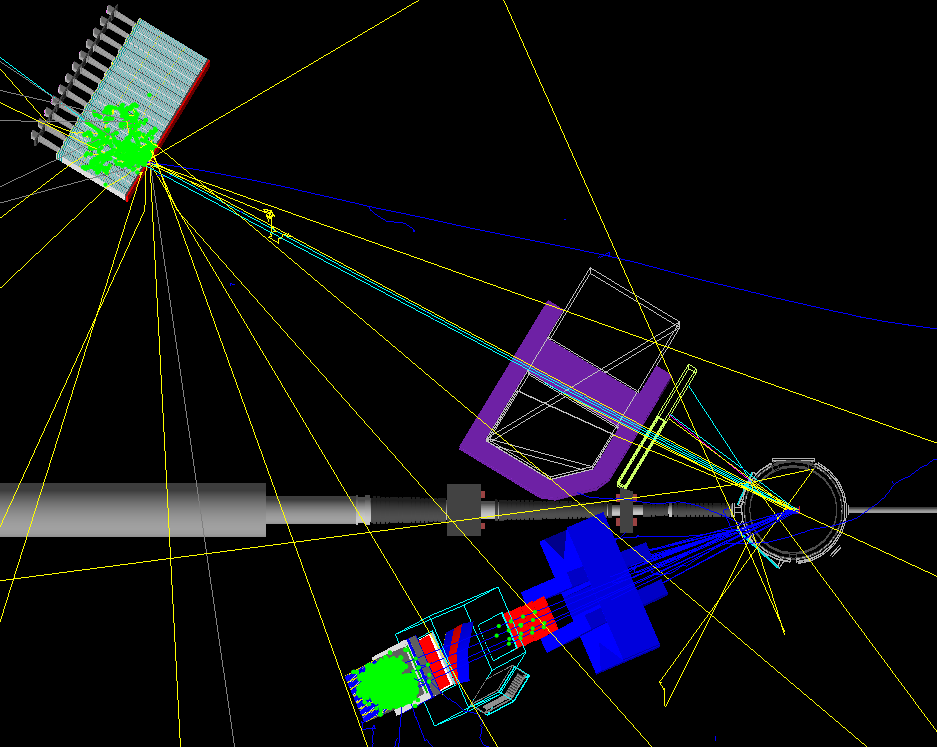
\includegraphics[width=9.6cm,height=8cm]{Plots/SetupHiEPoint.png}
    \caption{Top view of the experimental apparatus model in G4SBS, shown in the high $\epsilon$ configuration. The beam direction is indicated, as well as the main elements (HCal, SBS magnet, BigBite spectrometer)}
    \label{fig:g4sbssetup}
  \end{center}
\end{figure}
%
%Most of the subsystems are mostly accurately reproduced in G4SBS, using the correct 

\subsection{Background and trigger rates}

The main processes expected to contribute the trigger rates for the BigBite spectrometer are:
%
\begin{itemize}
\item{the inelastic electron nucleon scattering process;}
\item{photons from inclusive $\pi^0$ production;}
\item{and to a lesser extent, charged pions.}
\end{itemize}
%
One the other hand, we expect all sorts of hadronic backgrounds to contribute to the rates in HCal, the dominant ones being pions.
Both the inelastic scattering and the inclusive neutral and charged pion production are implemented in G4SBS, the latter relying on the Wiser parametrization \cite{wiser}.
We may also considered the minimum-bias ``beam-on-target'' generator for the HCal background, especially at lower angle (all electromagnetic and hadronic processes being built-in in G4SBS).

The thresholds to apply to each arm are determined as a function of the elastic peak.
For the electron arm, the threshold has been set at $\mu_E - 2.5 \sigma_E$,  $\mu_E$ and $\sigma_E$ being respectively the position and width of the fitted elastic peak. 
Fig.~\ref{fig:BBRates} presents the distributions of rate of energy deposit for the different processes involved in the BigBite trigger rates. 
%
\begin{figure}[!h]
  \begin{center}
    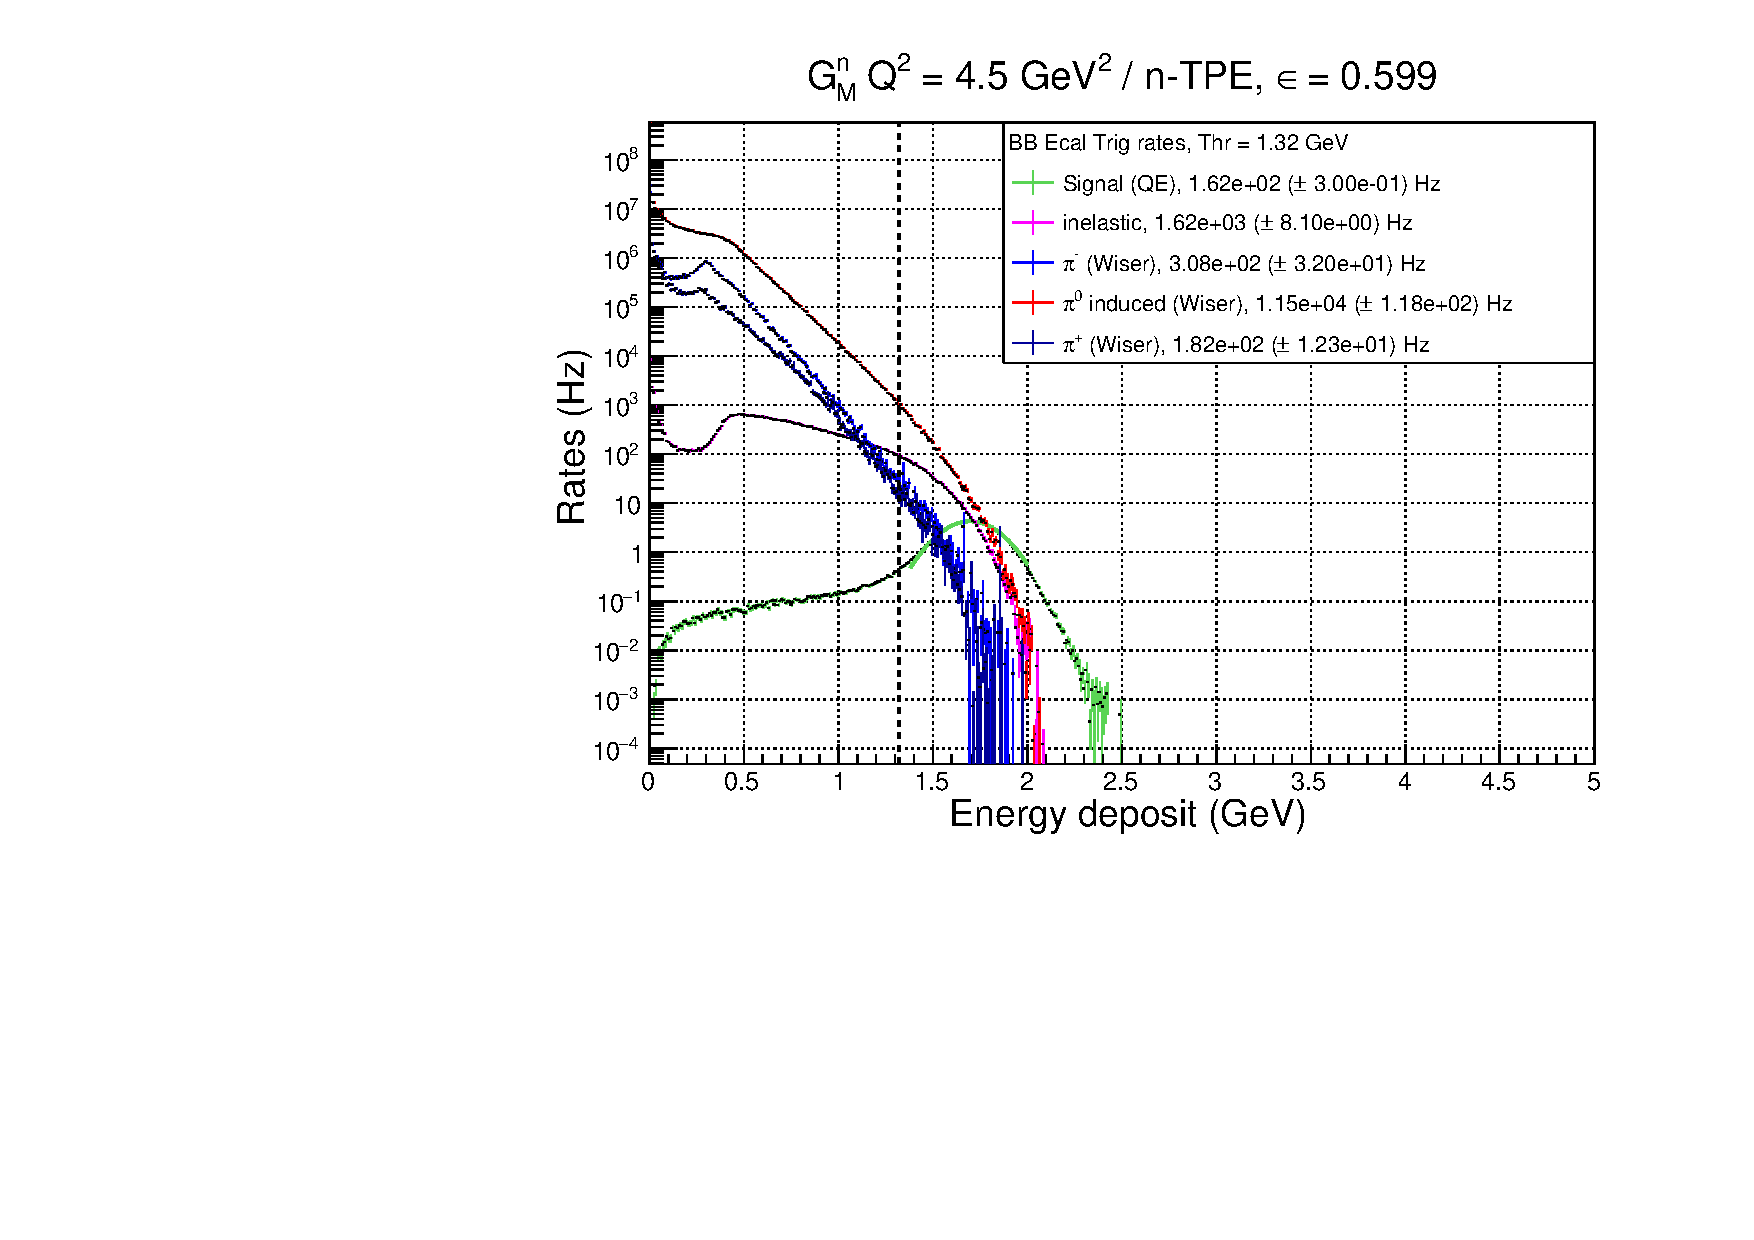
\includegraphics[width=6cm]{Plots/BBECalRates_gen-tpe_le.pdf}
    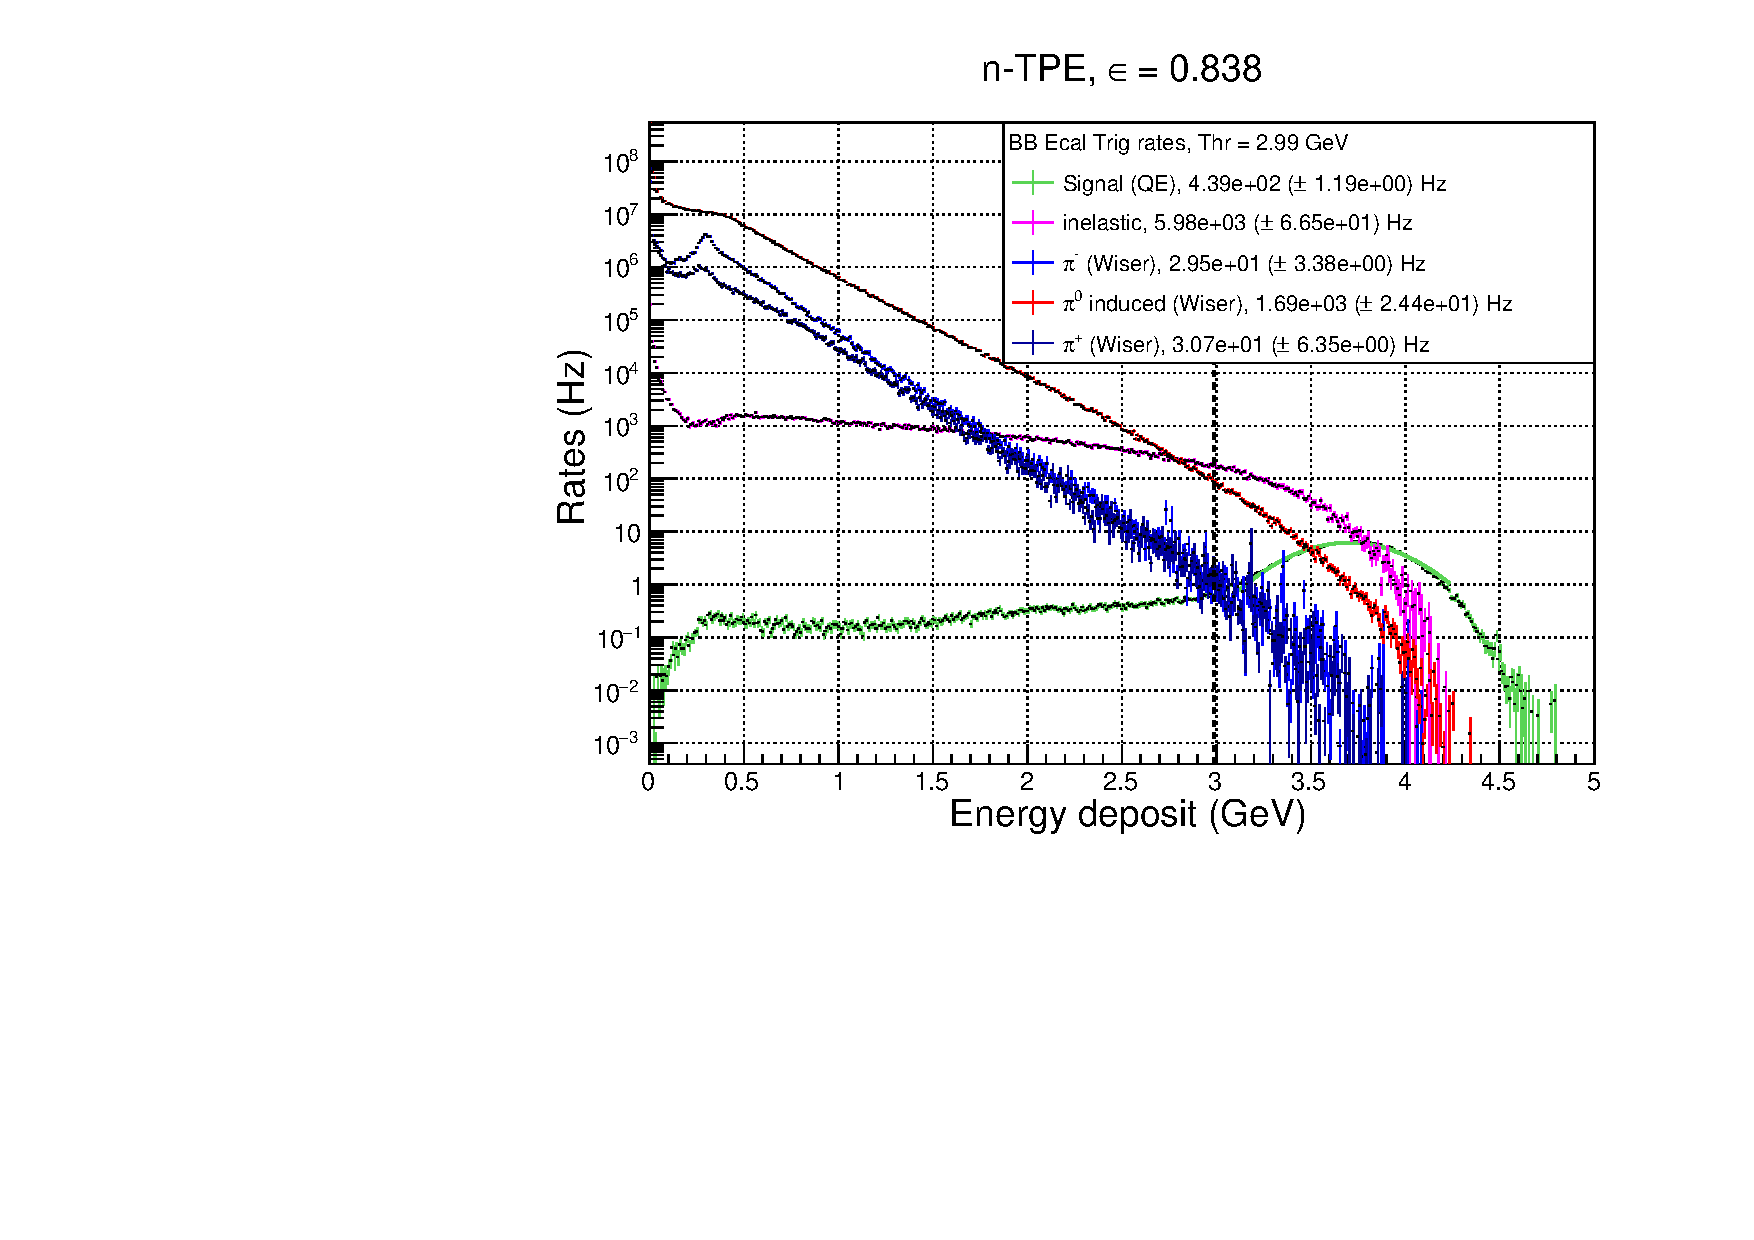
\includegraphics[width=6cm]{Plots/BBECalRates_gen-tpe_he.pdf}
    \caption{Rates of the different process contributing to the BigBite electron arm trigger, for the low $\epsilon$ (left) and the high $\epsilon$ (right). Quasi-elastic is in green, inelastic in magenta, $\pi0$ in red, $\pi^-$ in blue, and $\pi^+$ in dark blue. Note the resolution for the elastic peak in the BigBite shower is $\sim0.3$ GeV.}
    \label{fig:BBRates}
  \end{center}
\end{figure}
%

Since HCal is a sampling calorimeter (meaning that only a fraction of the shower energy is measured), it's resolution is significantly wider ($\sim0.7$ GeV).
Due to this, the threshold is at 90\% efficiency (which corresponds to $\sim$0.1 GeV for both kinematics.
Fig.~\ref{fig:HCalRates} presents the distributions of rate of energy deposit for the different processes involved in the BigBite trigger rates.
%
\begin{figure}[!h]
  \begin{center}
    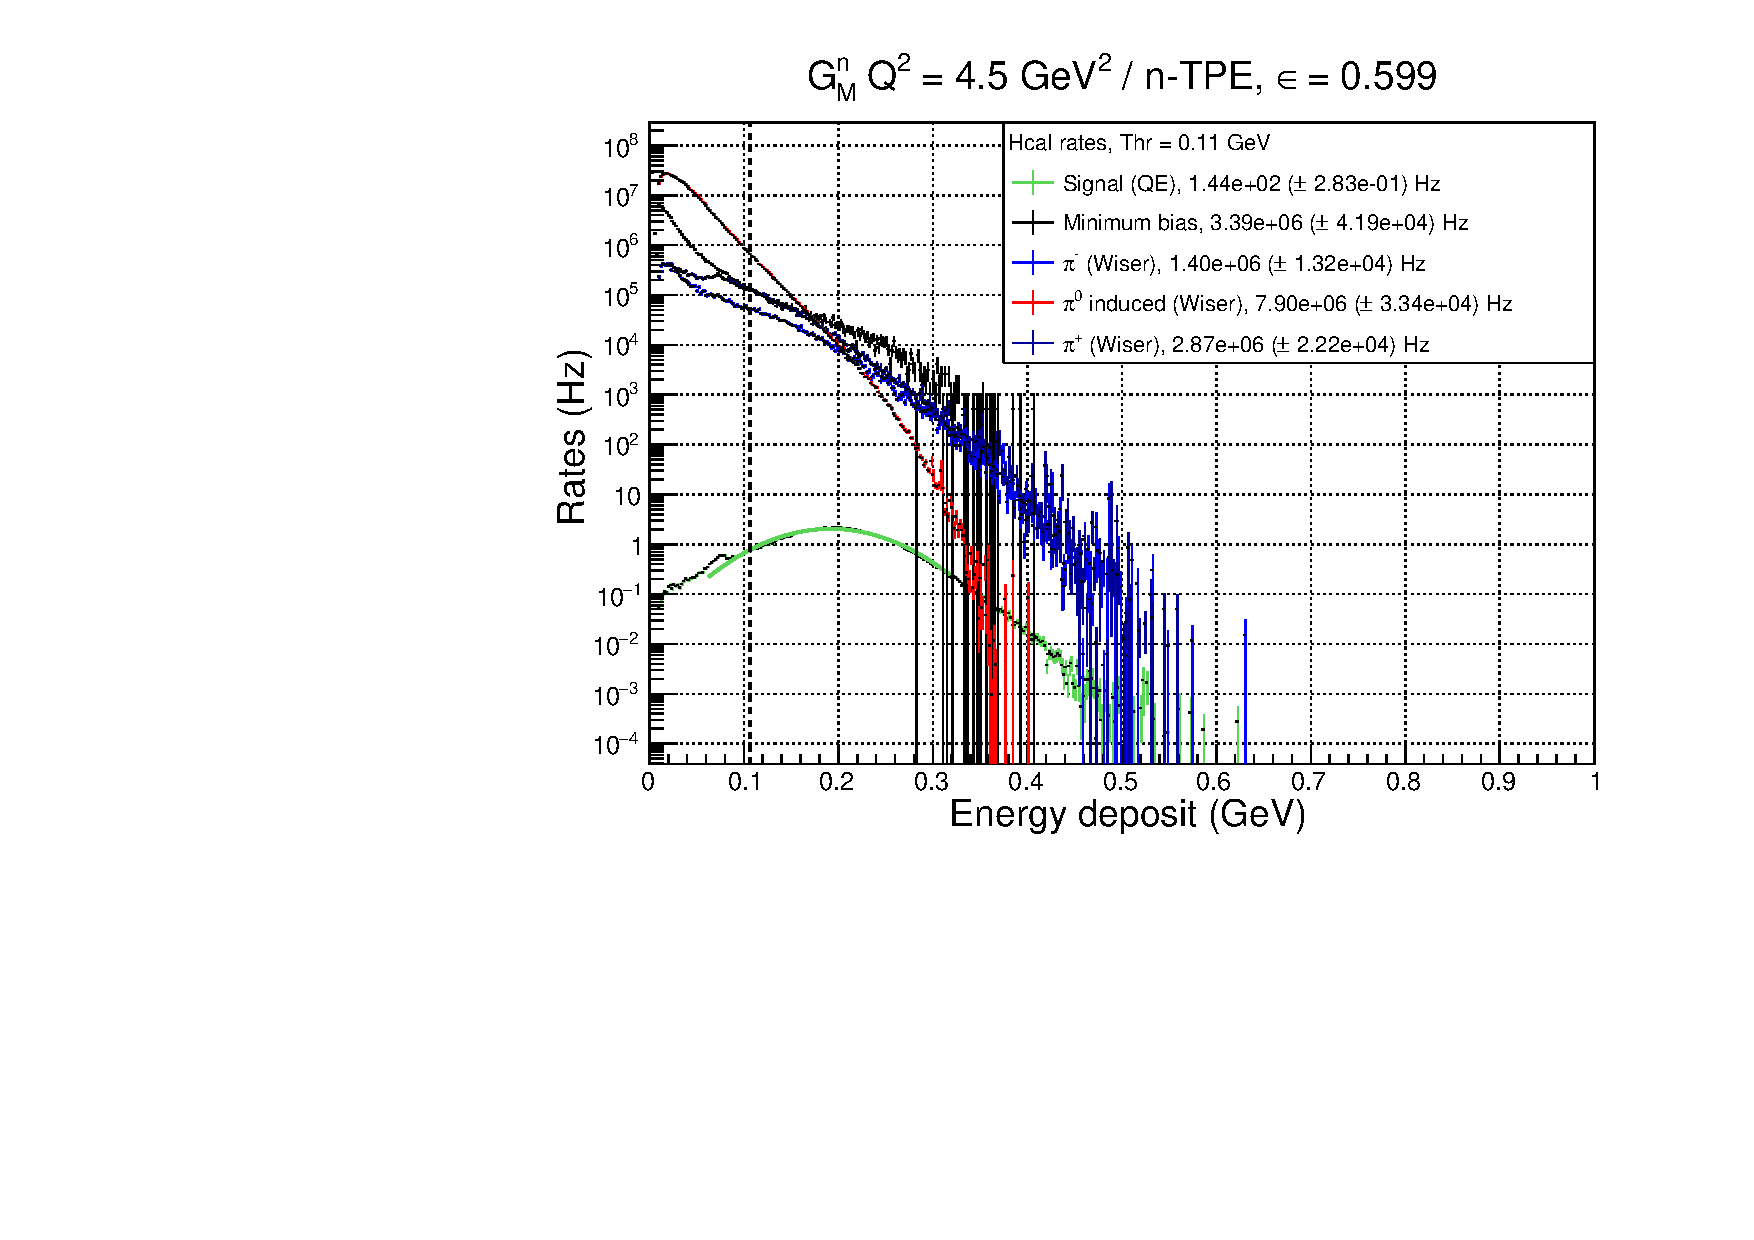
\includegraphics[width=6cm]{Plots/HCalRates_gen-tpe_le.pdf}
    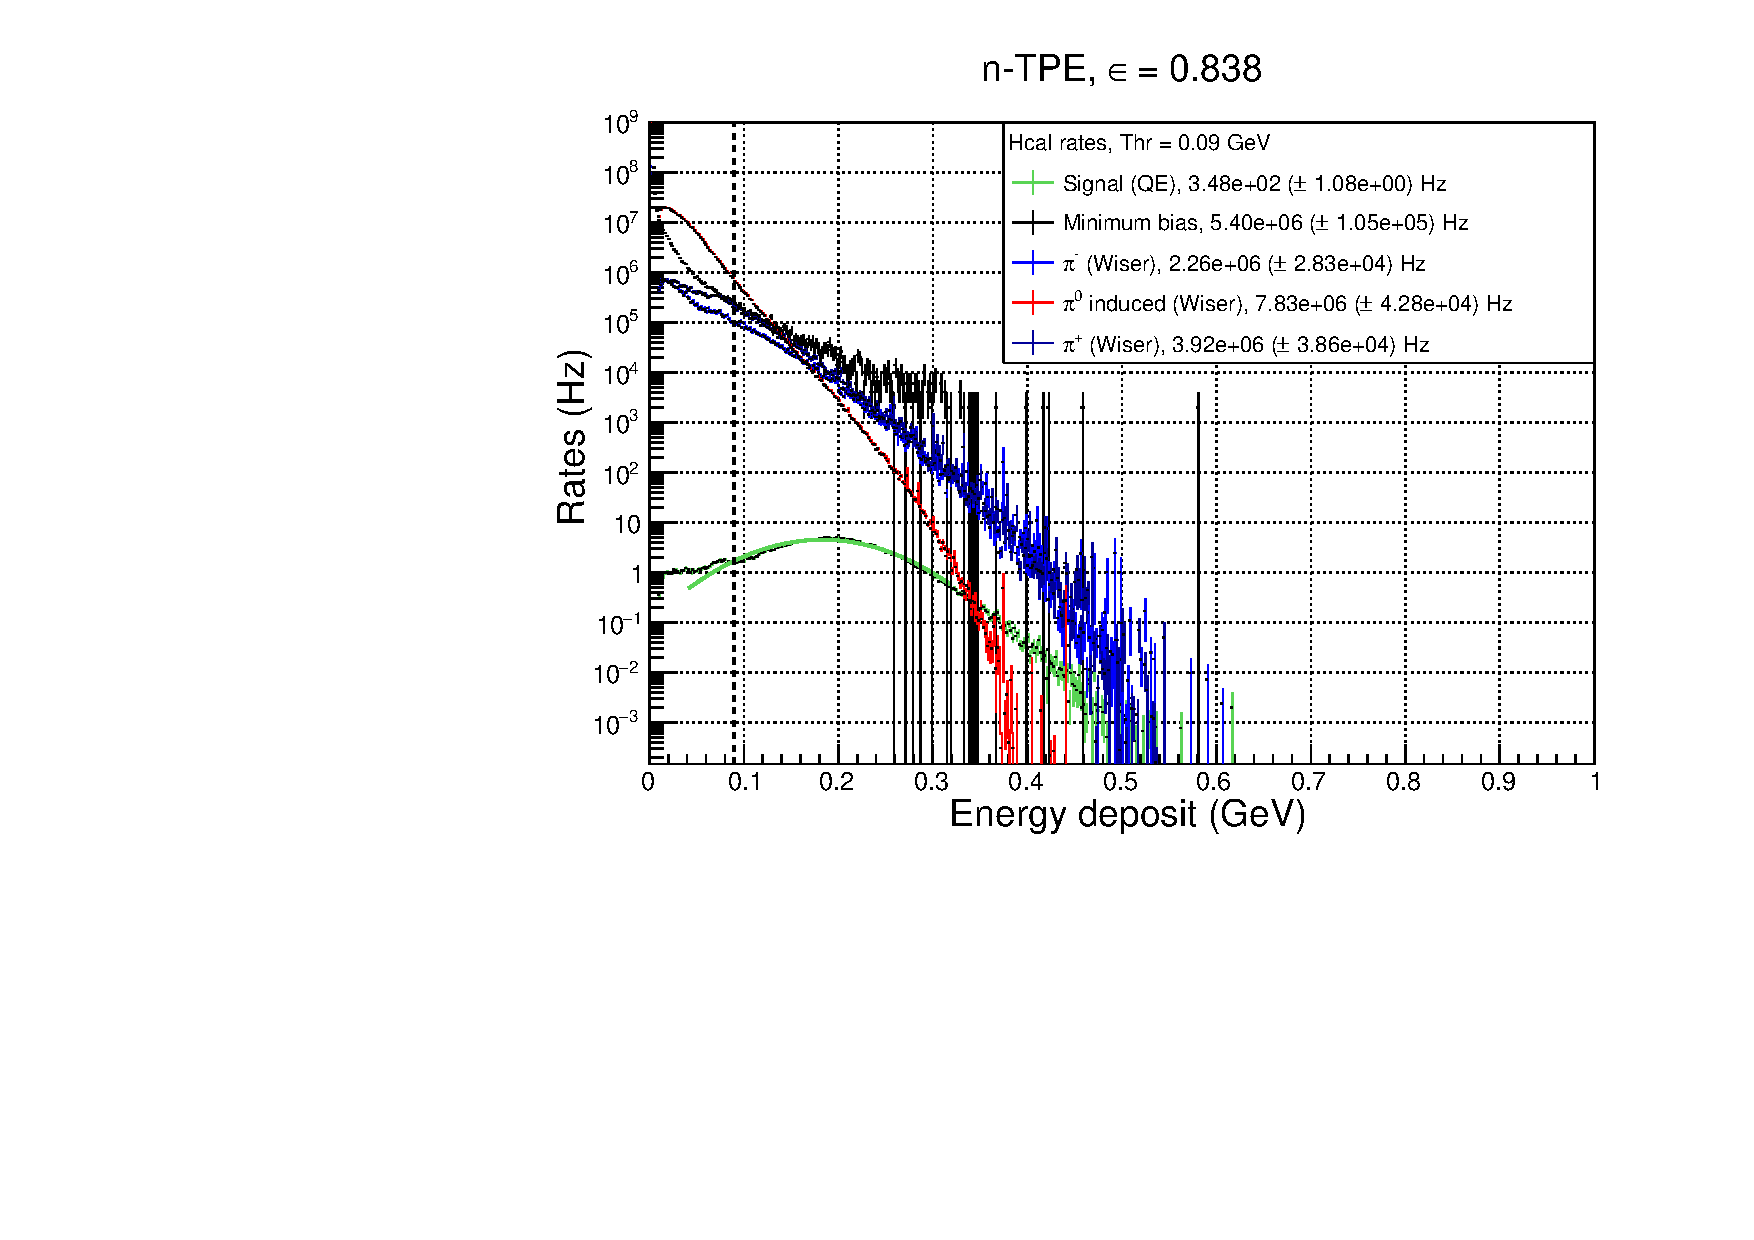
\includegraphics[width=6cm]{Plots/HCalRates_gen-tpe_he.pdf}
    \caption{Rates of the different process contributing to the HCal trigger, for the low $\epsilon$ (left) and the high $\epsilon$ (right). Quasi-elastic is in green, minimum bias in black, $\pi0$ in red, $\pi^-$ in blue, and $\pi^+$ in dark blue. Note the peak itself is around 0.2 GeV for 3.2 GeV nucleons.}
    \label{fig:HCalRates}
  \end{center}
\end{figure}
%

The thresholds and trigger rates for each arm, as well as the coincidence rate (assuming 30ns coincidence window), are summarized in Table.~\ref{tab:TrigRates}.
%
\begin{center}
\begin{table}[h]
\begin{tabular}{|l|c|c|c|c|}
\hline
Point ($\epsilon$) & \multicolumn{2}{|c|}{1 (0.599)} & \multicolumn{2}{c|}{2 (0.838)} \\
\hline
& BigBite & HCal & BigBite & HCal \\ 
& rates (Hz) & rates (Hz) & rates (Hz) & rates (Hz) \\
\hline
threshold (GeV) & 1.32 & 0.106 & 2.99 & 0.090 \\
\hline
Quasi-elastic   & 1.62$\times 10^{2}$ & 1.44$\times 10^{2}$ & 4.39$\times 10^{2}$ & 3.48$\times 10^{2}$ \\
Inelastic       & 1.62$\times 10^{3}$ & - & 5.98$\times 10^{3}$ & - \\
$\pi^-$ (Wiser) & 3.08$\times 10^{2}$ & 1.40$\times 10^{6}$ & 2.95$\times 10^{2}$ & 1.96$\times 10^{6}$ \\
$\pi^0$ (Wiser) & 1.15$\times 10^{4}$ & 7.90$\times 10^{6}$ & 1.69$\times 10^{3}$ & 5.77$\times 10^{6}$ \\
$\pi^+$ (Wiser) & 1.82$\times 10^{2}$ & 2.87$\times 10^{6}$ & 3.07$\times 10^{2}$ & 3.34$\times 10^{6}$ \\
Minimum bias    & - & 3.39$\times 10^{6}$ & - & 3.32$\times 10^{6}$($^*$) \\ 
\hline
{\em Total} & 1.37$\times 10^{4}$ & 1.22$\times 10^{7}$ & 8.17 $\times 10^{3}$ & 1.11$\times 10^{7}$ \\
(min. bias - HCal only) &  & / 3.39$\times 10^{6}$ &  & / 3.32$\times 10^{6}$ \\
\hline
{\bf Coincidence rate} & \multicolumn{2}{|c|}{5.01$\times 10^{3}$} & \multicolumn{2}{c|}{2.72$\times 10^{3}$} \\
(with min. bias HCal) & \multicolumn{2}{|c|}{1.39$\times 10^{3}$} & \multicolumn{2}{|c|}{8.14$\times 10^{2}$} \\
\hline
\end{tabular} 
\caption{Trigger rates for BigBite and HCal, with the different process contributions separated, and the sum. For HCal, the total rates is either the sum of the (Wiser) inclusive pions or the minimum bias. The coincidence rates assume a 30 ns coincidence window.}
\label{tab:TrigRates}
\end{table}
\end{center}
%
Note that for HCal, the ``total rates'' is either the sum of inclusive charged and neutral pions evaluated with the Wiser cross sections {\em or} the ``minimum bias'' beam on target. We have good reasons to think that the Wiser code results actually overestimate the HCal rates, but for the sake of thoroughness, we have checked the coincidence rates assuming the sum of the inclusive pions (evaluated with the Wiser cross sections) as the HCal rates.

In the worst case scenario, the coincidence rates could be as high as 5kHz, which might be at the limit of manageability for the DAQ.
However, a slight increase on the HCal threshold (which would drop the efficiency from $\sim$90\% to $\sim$85\%) would decrease the total HCal rates by $\sim$35\% to 40\% in this worst case scenario, which would make the situation more manageable (3.3 kHz).

\subsection{Accidentals: contamination from inelastic}

The main source of contamination for the quasi-elastic comes from the inelastic electron-nucleon scattering. Most of this contamination can be cleaned out thanks to a selection on the center of mass energy
%
\begin{equation}
  W^2 = M_{N}^2+2M_{N}^{2}(E-E')-Q^2, %= (q+p)^2 
\end{equation}
%
and the missing transverse momentum of the nucleon
%
\begin{equation}
  p_{\perp miss} = \sqrt{(q_{x}-p'_{x})^2+(q_{y}-p'_{y})^2},
\end{equation}
%
where $M_N$ is the mass of the nucleon, $E$ and $E'$ the initial and final energy of the electron, and $q_{x,y}$, $p'_{x, y}$ are the projections on $x$, $y$ of the vectors of the virtual photon and final nucleon.
The distributions of these quantities (weighted with cross section and including detector resolutions) are displayed for quasi-elastic and inelastic scattering, and for proton and nucleon, on Fig.~\ref{fig:inel_contam_le} for the low $\epsilon$ kinematic, and on Fig.~\ref{fig:inel_contam_he} for the high $\epsilon$ kinematic.
%
\begin{figure}[!h]
  \begin{center}
    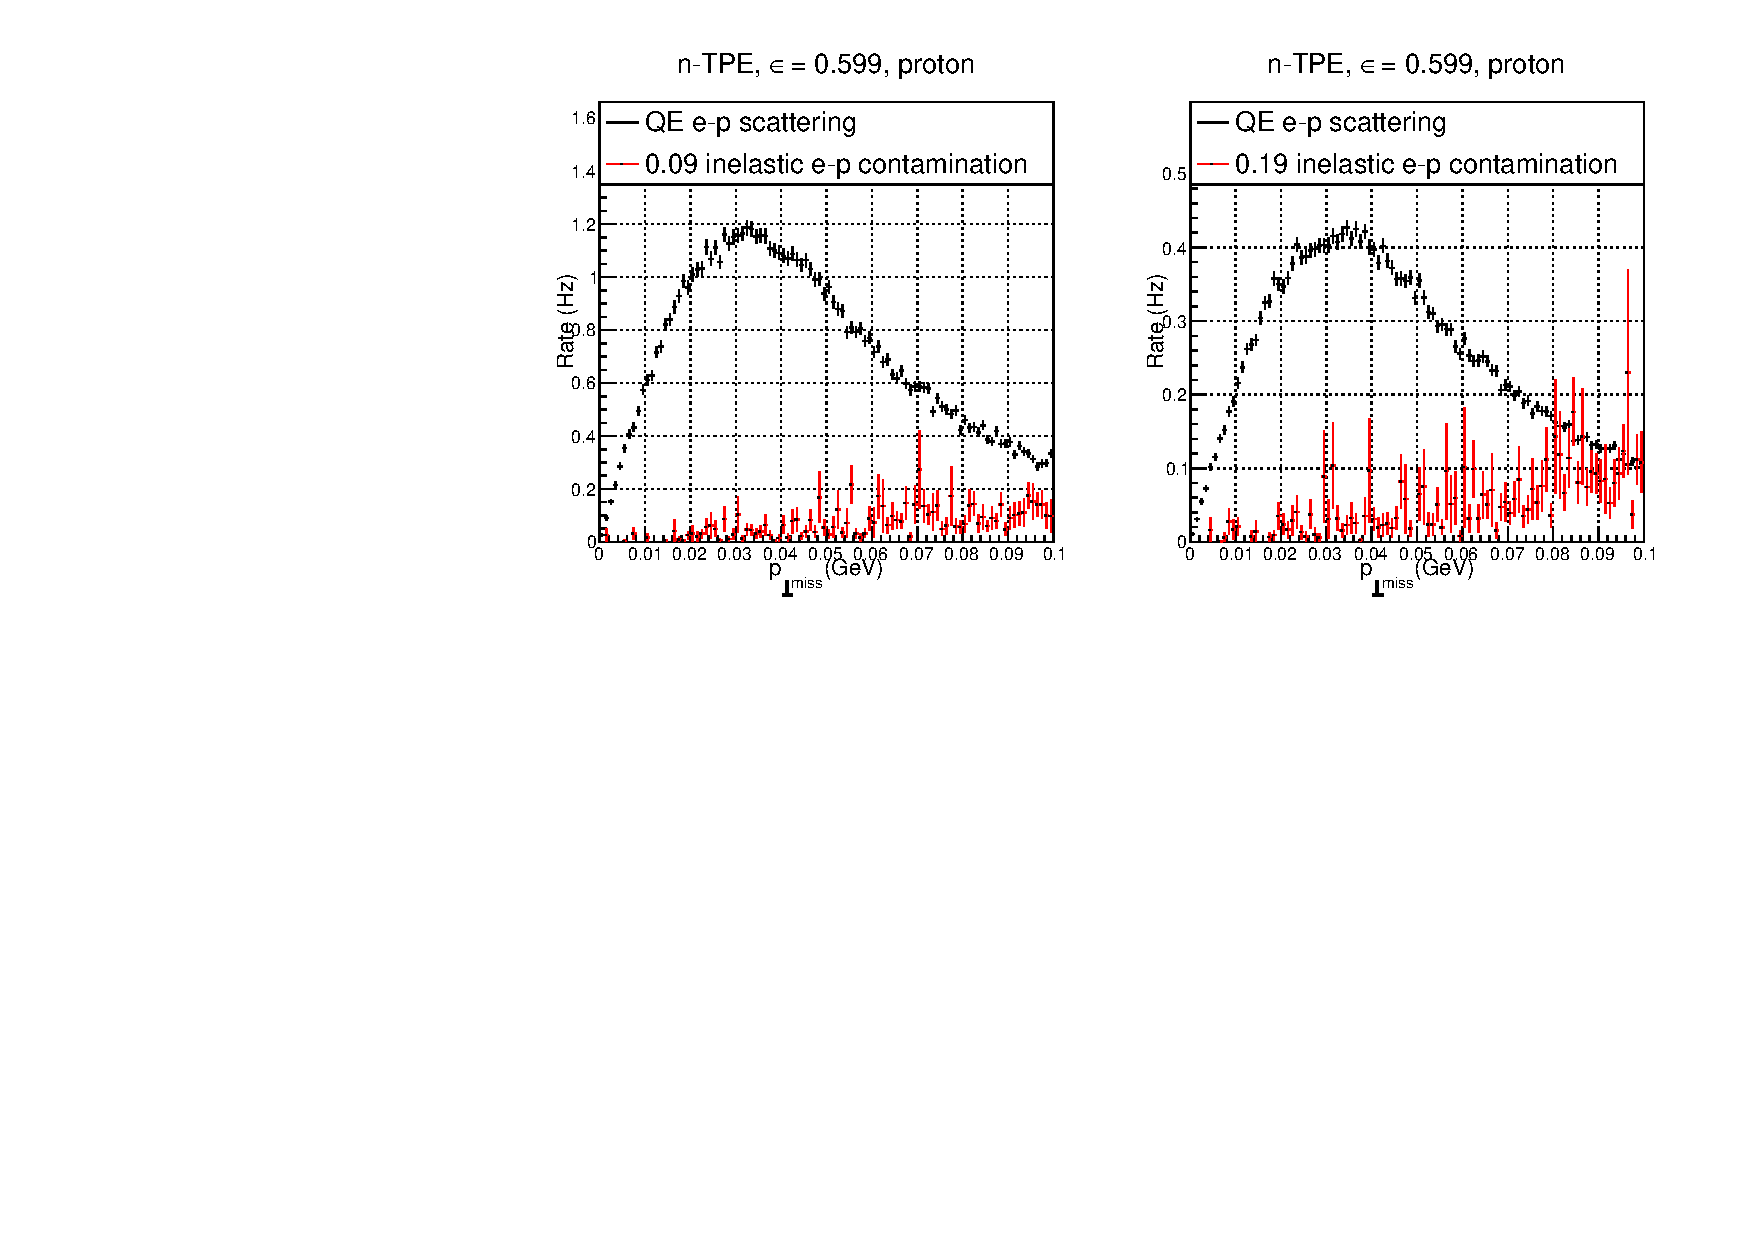
\includegraphics[width=12cm]{Plots/gen-tpe_le_pperp_acc.pdf}
    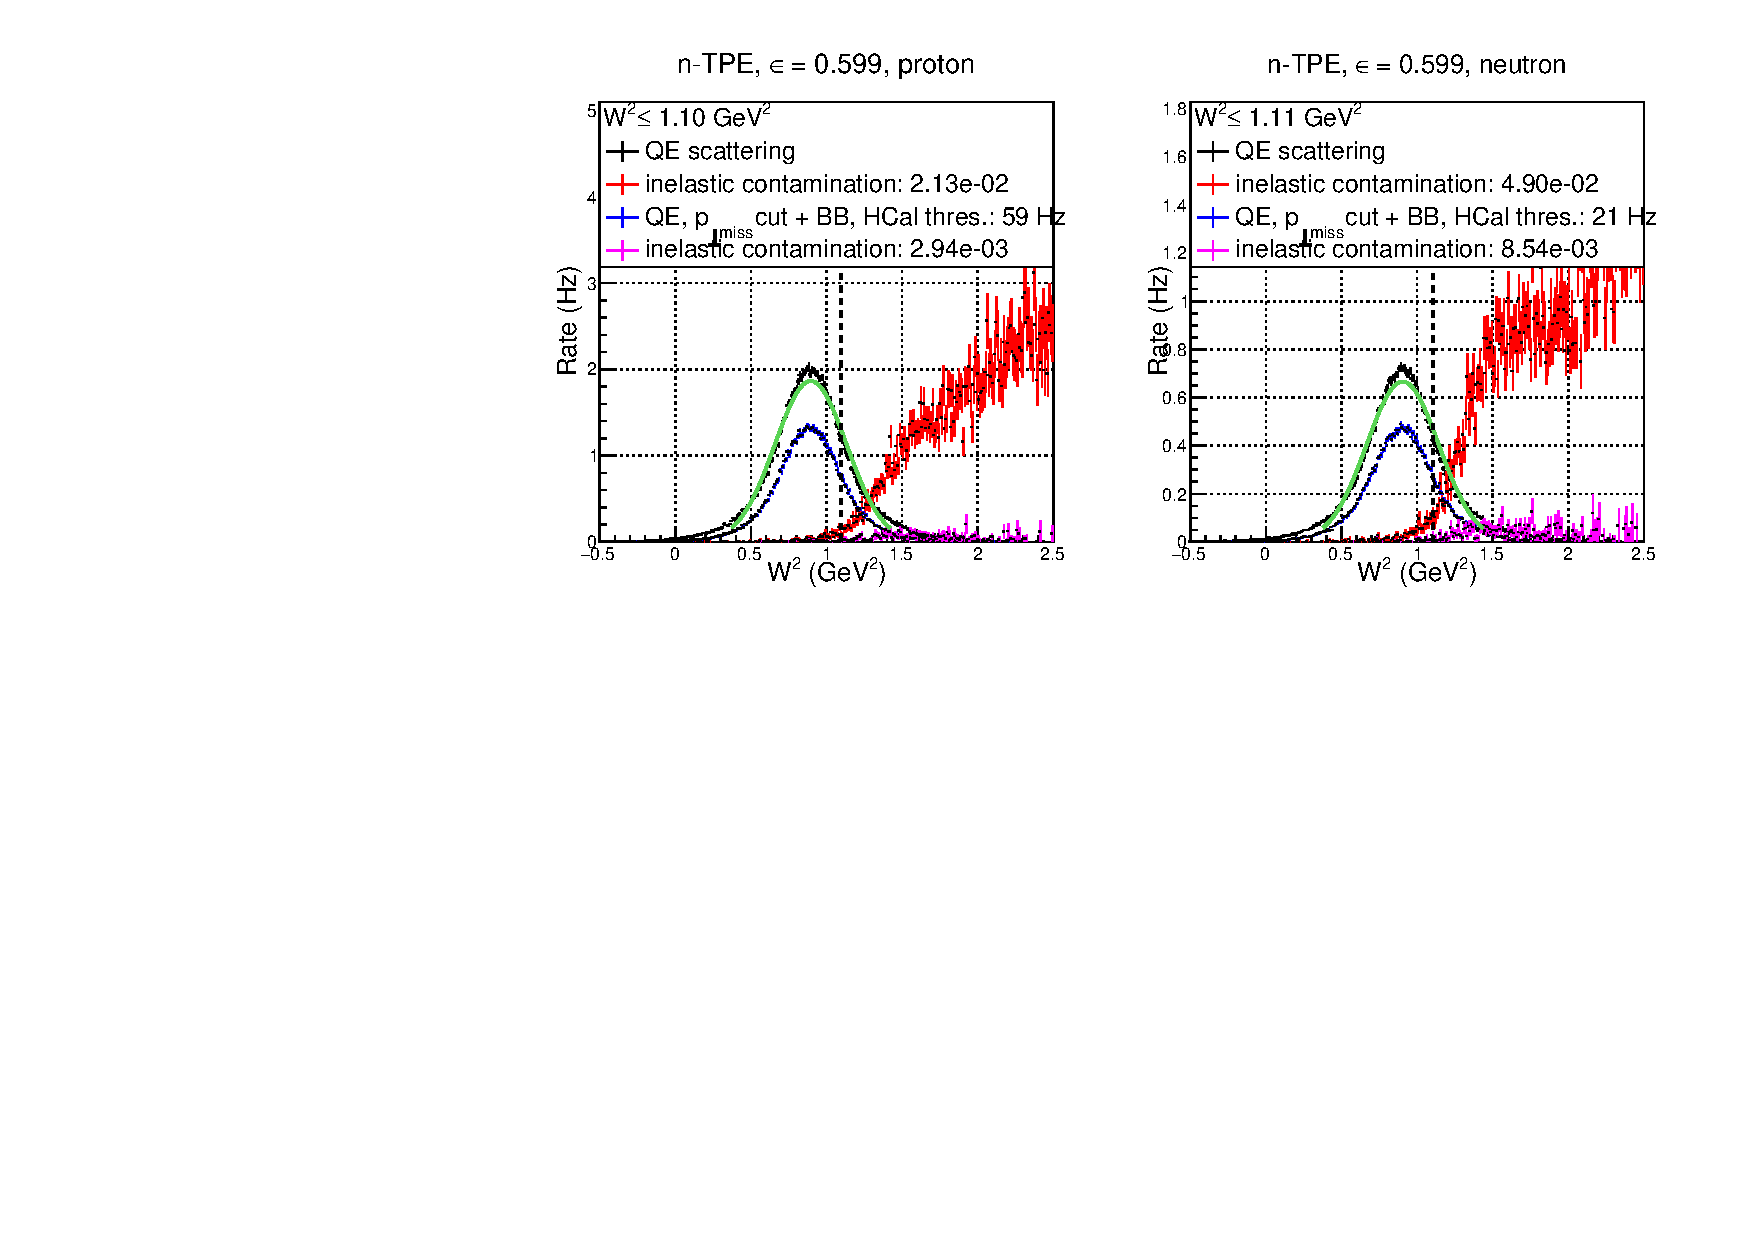
\includegraphics[width=12cm]{Plots/gen-tpe_le_W2_acc.pdf}
    \caption{Compared quasi-elastic and inelastic distributions (including detectors resolutions) for $p_{\perp miss}$ (top) and $W^2$ (bottom), for the low $\epsilon$ kinematic. Comparison for protons is on the left, and comparison for neutrons is on the right. On the bottom panel, black and red are before the $p_{\perp miss}~\leq~0.1~\mathrm{GeV}$ selection, while blue and magenta are after $p_{\perp miss}~\leq~0.1~\mathrm{GeV}$ selection and application of BigBite shower and HCal thresholds.}
    \label{fig:inel_contam_le}
  \end{center}
\end{figure}
%
\begin{figure}[!h]
  \begin{center}
    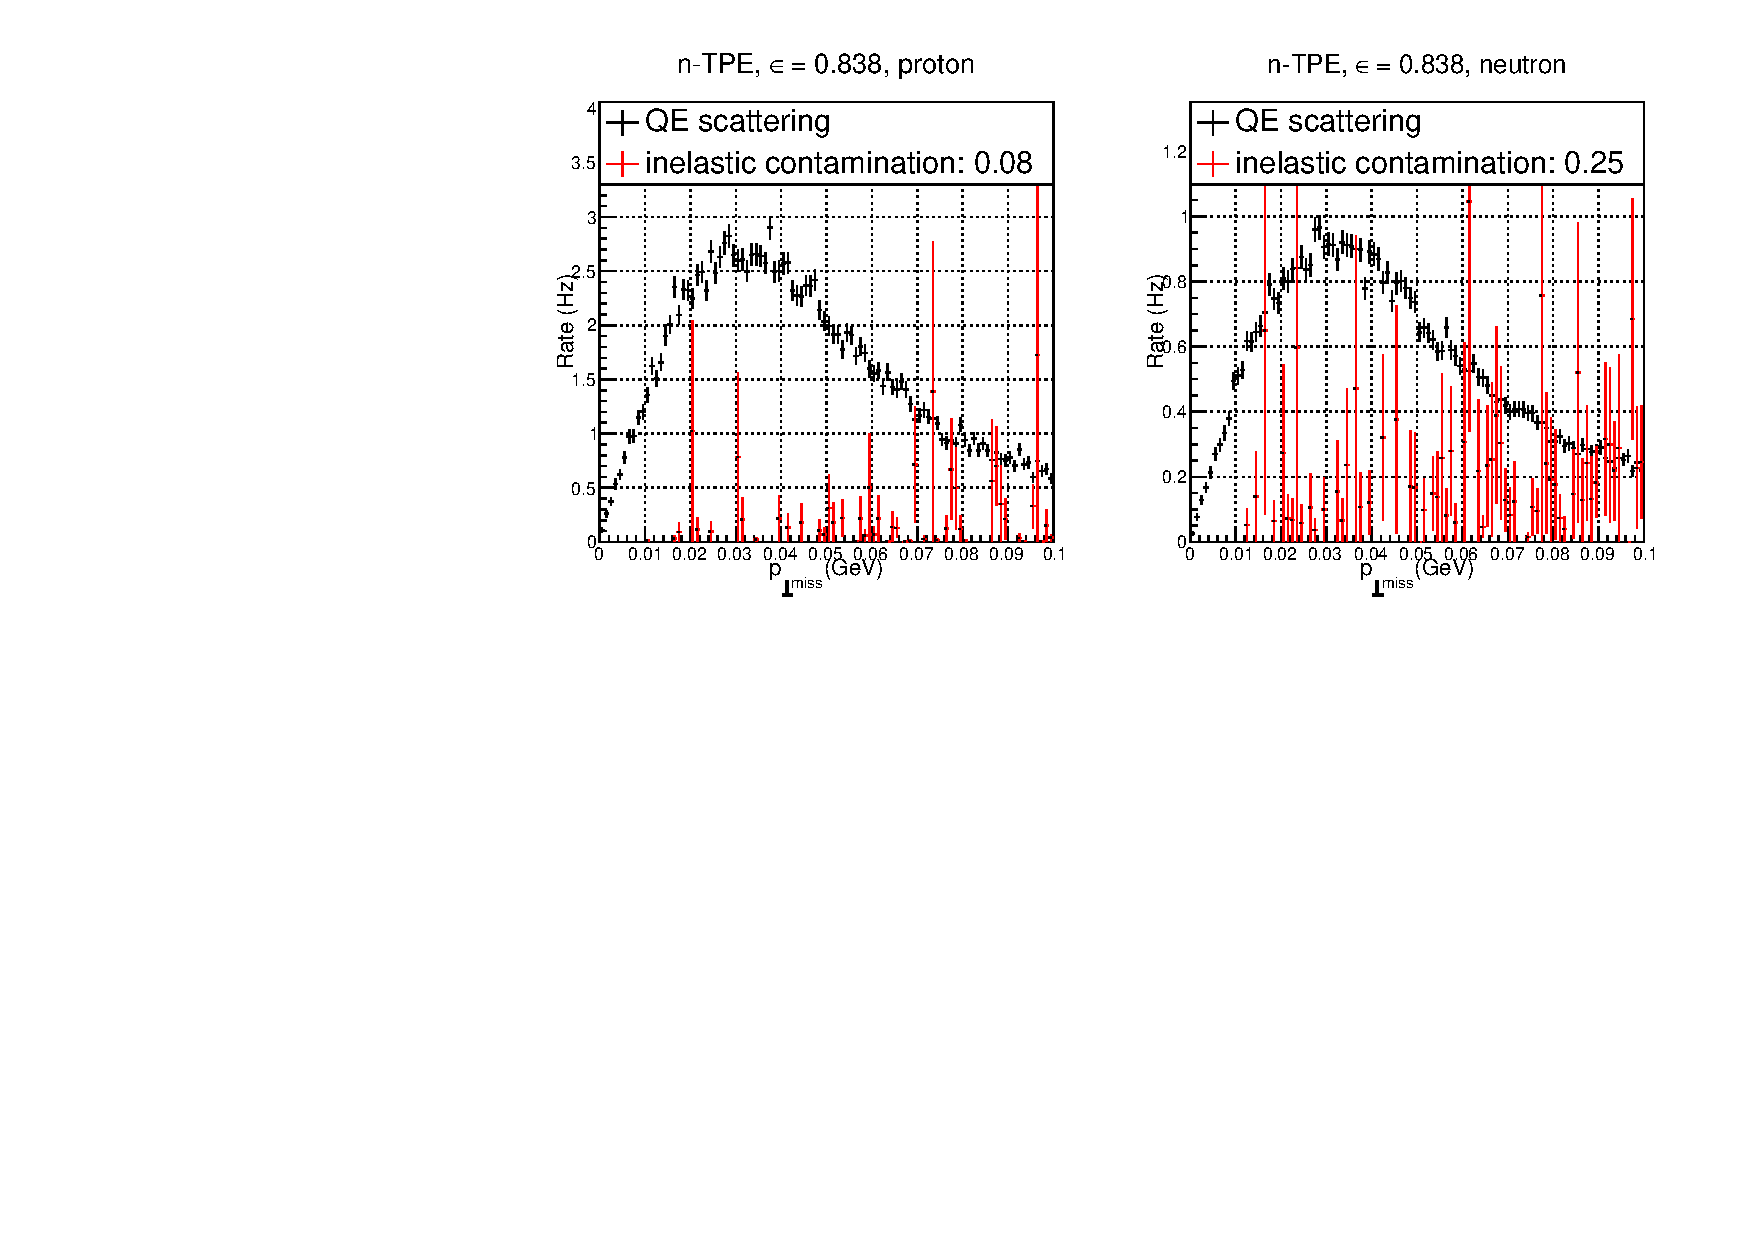
\includegraphics[width=12cm]{Plots/gen-tpe_he_pperp_acc.pdf}
    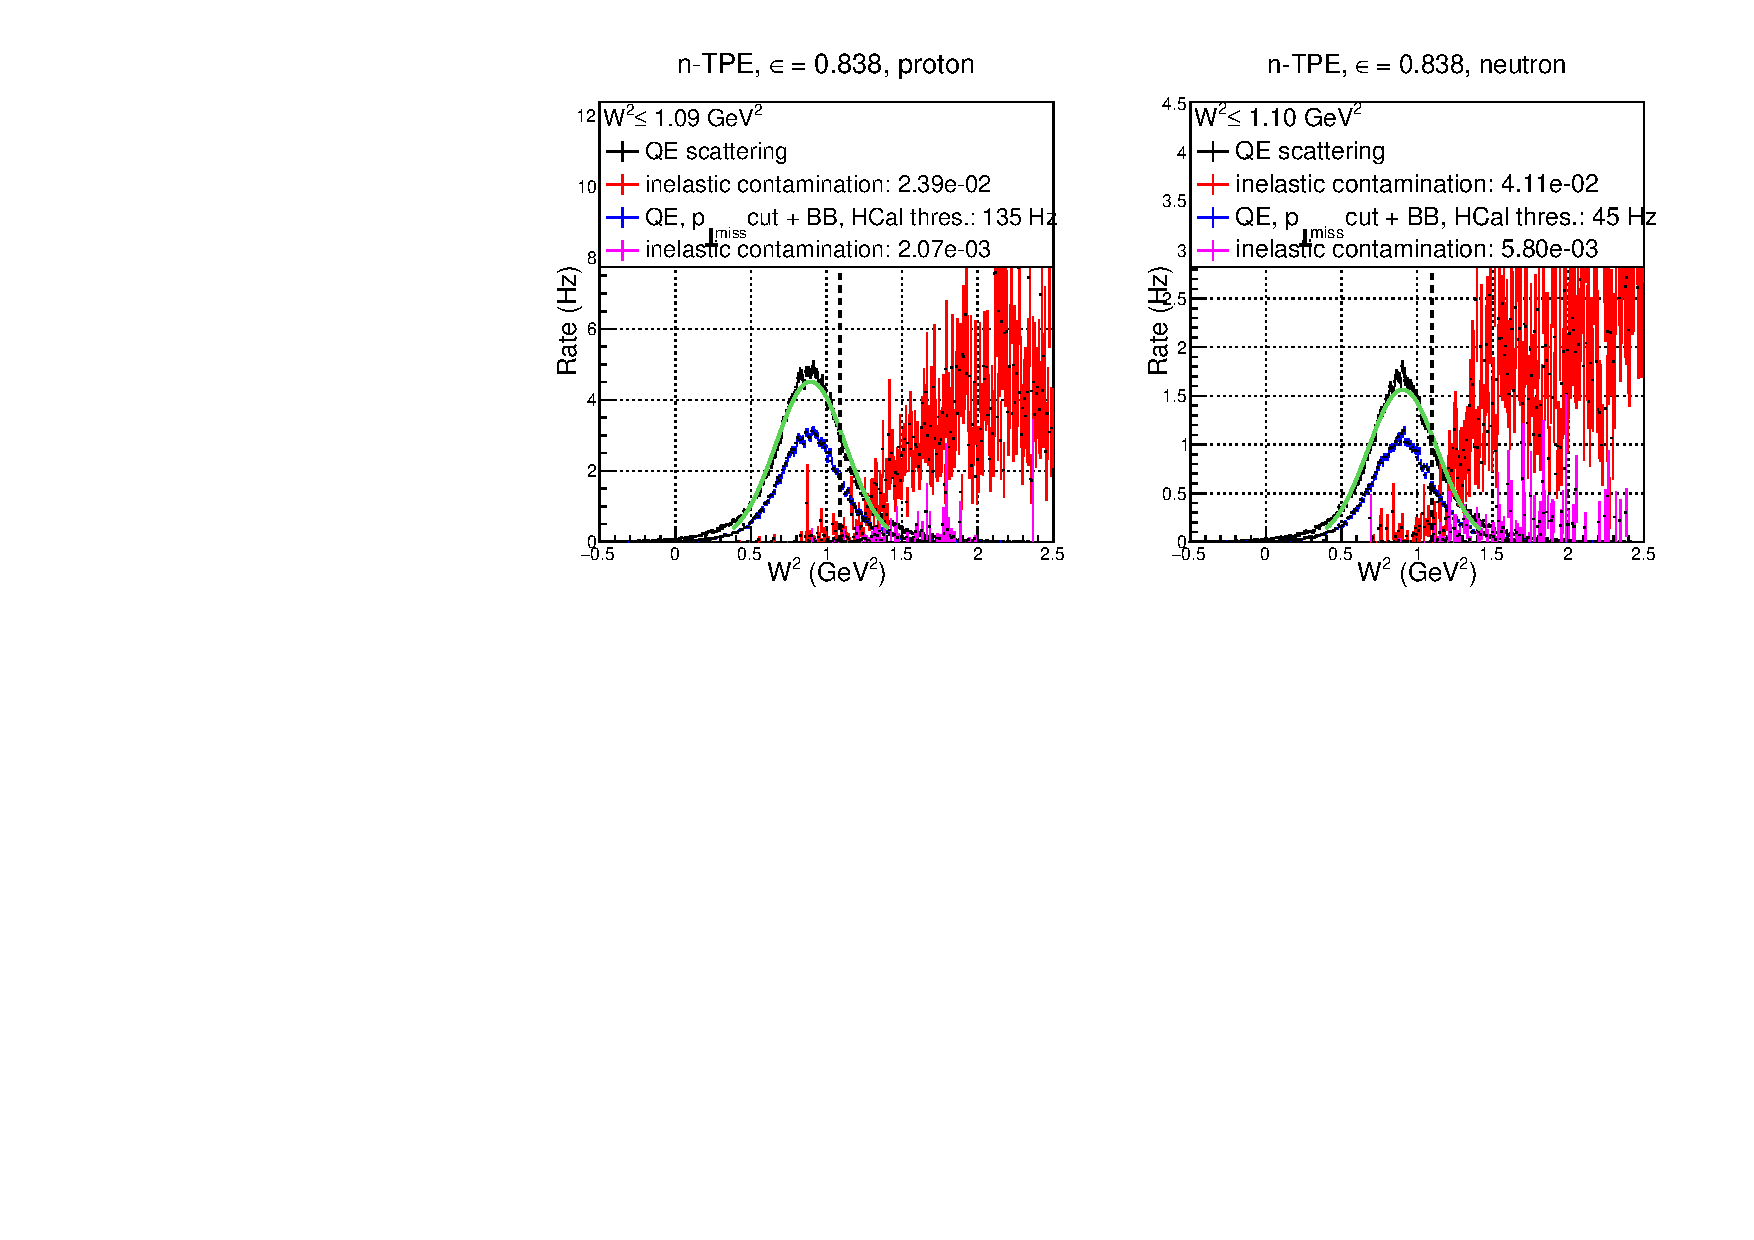
\includegraphics[width=12cm]{Plots/gen-tpe_he_W2_acc.pdf}
    \caption{Compared quasi-elastic and inelastic distributions (including detectors resolutions) for $p_{\perp miss}$ (top) and $W^2$ (bottom), for the high $\epsilon$ kinematic. Comparison for protons is on the left, and comparison for neutrons is on the right. On the bottom panel, black and red are before the $p_{\perp miss}~\leq~0.1~\mathrm{GeV}$ selection, while blue and magenta are after $p_{\perp miss}~\leq~0.1~\mathrm{GeV}$ selection and application of BigBite shower and HCal thresholds.}
    \label{fig:inel_contam_he}
  \end{center}
\end{figure}
%
Provided that we are not limited by statistics and the sample purity is capital for our experiment, we set the selection criteria on $W^2$ and $p_{\perp miss}$ to maximize inelastic contamination (ideally below 1~\%). 
Setting $p_{\perp miss}~\leq~0.1~\mathrm{GeV}$ and $W^2~\leq~1.1~\mathrm{GeV}^2$, the inastic contamination of the elastic sample ranges from 0.2~\% to 0.9~\%, while rataining $\geq$~60~\%. % of statistics listed in Table.~\ref{tab:Rates}

\subsection{Quasi-elastic counting rates}

The signals for this experiment have been generated using the G4SBS elastic/quasi-elastic generator. 
We generated 1M events sample for each kinematics, on a solid angle that was larger than the detector acceptance.
To evaluate the detector solid angle, we define simple criteria that each event has to pass, defined as the following;
%
\begin{itemize}
\item{require a primary track, going through all 5 GEM layers (electron arm);}
\item{require non-zero energy deposit in both the preshower and shower (electron arm);}
\item{require non-zero energy deposit in HCal (hadron arm).}
\end{itemize}
%
The detector solid angle, for both proton and neutron, are defined in Table.~\ref{tab:kinExpParams}
%
\begin{center}
\begin{table}[h]
  %\begin{tabular}{|>{\centering}m{0.3in} |>{\centering}m{0.55in}|>{\centering}m{0.4in}| >{\centering}m{0.4in}| >{\centering}m{0.45in}|>{\centering}m{0.45in}|>{\centering}m{0.4in}|>{\centering}m{0.4in}|>{\centering\arraybackslash}m{0.4in}|}
\begin{tabular}{|c|c|c|c|}
\hline
Point ($\epsilon$) & $\Delta\Omega_e$ & $\Delta\Omega_e \otimes \Delta\Omega_n$ & $\Delta\Omega_e \otimes \Delta\Omega_p$ \\
 & (msr) & (msr) & (msr) \\
\hline
1 (0.599) & 52.4 & 46.7 & 47.2 \\
\hline
2 (0.838) & 32.7 & 20.8 & 22.2 \\
\hline
\end{tabular} 
\caption{Kinematics electron solid angle, and convoluted electron/hadron solid angle}
\label{tab:kinExpParams}
\end{table}
\end{center}
%
Then, we evaluate the detection efficiency. For the electron, we require the energy reconstructed in the BigBite calorimeter to be above a threshold defined as $thr = \mu_E- 2.5* \sigma_E$, as well as a minimum number of GRINCH PMTs fired due to the primary electron; For HCal, we require the threshold to be such as we obtain ~90\% efficiency. These values are summarized in Table.~\ref{tab:kinEffs}.
%
\begin{center}
\begin{table}[h]
\begin{tabular}{|c|c|c|c|c|c|c|c|}
\hline
Point ($\epsilon$) & BB thr. & HCal thr. & $\eta_{det~e}$ & $\eta_{det~n}$ & $\eta_{det~p}$ & $\eta_{sel~n}$ & $\eta_{sel~p}$ \\
 & (GeV) & (GeV) &  &  &  &  &  \\
\hline
1 (0.599) & 1.32 & 0.11 & 0.902 & 0.904 & 0.892 & 0.589 & 0.605 \\ 
\hline
2 (0.838) & 2.99 & 0.09 & 0.808 & 0.889 & 0.882 & 0.617 & 0.647 \\
\hline
\end{tabular} 
\caption{Kinematics electron thresholds, particle detection efficiencies ($\eta_{det}$), and efficiency of quasi-elastic selection $\eta_{sel}$ separated for the proton and the neutron.}
\label{tab:kinEffs}
\end{table}
\end{center}
%

The counting rates are evaluated using the events that have passed the selection described above, and weighting those events with the cross section calculated by G4SBS, multiplied by the generation solid angle, using the formula:
%
\begin{equation}
  N_{est} = {\cal L} \Delta t \times \sum_{i \in accepted~evts} \frac{d\sigma}{d\Omega} *\Delta\Omega_{Gen} /N_{Gen}
\end{equation}
%
Events are ``accepted'' if they meet the following criteria:
%
\begin{itemize}
\item{the electron is in the BigBite acceptance};
\item{the electron passes the BigBite threshold defined in Table~\ref{tab:kinEffs} and gives signal in the GRINCH;}
\item{the nucleon is in the HCal acceptance and passes the HCal threshold defined in Table~\ref{tab:kinEffs};}
\item{the event passes the quasi-elastic selection defined in the previous section {\it i.e.} $W^2~\leq~1.1~\mathrm{GeV}^2$ and $p_{\perp miss}~\leq~0.10~\mathrm{GeV}$.} 
\end{itemize}
%

The counting rates, as well as the reduced cross section $F^2$
and its error $\Delta F^2 = F^2/\sqrt{N_{QE}}$ are compiled for both kinematics in Table.~\ref{tab:Rates}, assuming a running time $\Delta t = 12$~hours of running at a beam intensity of $I_{exp} =~30~\mu$A on a liquid deuterium target with length $l_{tgt}~=~15$~cm and density $d_{tgt}~=~0.169~\mathrm{g.cm}^{-3}$.
%
\begin{center}
\begin{table}[h]
  %\begin{tabular}{|>{\centering}m{0.3in} |>{\centering}m{0.55in}|>{\centering}m{0.4in}| >{\centering}m{0.4in}| >{\centering}m{0.45in}|>{\centering}m{0.45in}|>{\centering}m{0.4in}|>{\centering}m{0.4in}|>{\centering\arraybackslash}m{0.4in}|}
\begin{tabular}{|c|c|c|c|c|c|c|}
\hline
Point ($\epsilon$) & QE $e$-$n$ & QE $e$-$p$ & $F^2_n$ & $\Delta F^2_n$ & $F^2_p$ & $\Delta F^2_p$ \\
 & counts & counts & ($\times 10^{-3}$) & ($\times 10^{-6}$) & ($\times 10^{-3}$) & ($\times 10^{-6}$) \\
\hline
1 (0.599) & 9.07$\times 10^{5}$ & 2.55$\times 10^{6}$ & 0.99 & 1.04 & 2.73 & 1.70 \\
\hline
2 (0.838) & 1.94$\times 10^{6}$ & 5.83$\times 10^{6}$ & 0.72 & 0.52 & 1.93 & 0.80 \\
\hline
\end{tabular} 
\caption{Quasi-elastic counting rates, and ``reduced cross section'' as defined by Eq.~\ref{eq:F2}. These rates assume $\Delta t = 12$~hours of running at a beam intensity of $I_{exp} =~30~\mu$A on a liquid deuterium target with length $l_{tgt}~=~15$~cm and density $d_{tgt}~=~0.169~\mathrm{g.cm}^{-3}$}%({\em preliminary})
\label{tab:Rates}
\end{table}
\end{center}
%

The expression of $F_2$ is: 
%
\begin{equation}
  F^2 = \frac{N_{QE}}{{\cal{L}}_{exp} \cdot \Delta t \cdot  d\sigma_{Mott}/d\Omega  \cdot \Delta\Omega \cdot  \eta}
  \label{eq:F2}
\end{equation}
%
where $\Delta t$ the running time, $\Delta\Omega$ is the convoluted BigBite-HCal solid angle, $\eta$ is the product of all efficiencies (detection efficiencies $\eta_{det}$ $\times$ selection efficiency $\eta_{sel}$)
%($\eta = \eta_{det~e} \times \eta_{det~n/p}  \times \eta_{QE sel~n/p}$)
, and ${\cal{L}}_{exp}$ is the experimental luminosity:
%
\begin{equation}
  {\cal{L}}_{exp} = \frac{I_{exp}}{q_e}*L_{tgt}*d_{tgt}\frac{\cal{N}_A}{m_{D}}.
\end{equation}
%
The calculation of the $F_2$ term requires the evaluation of the Mott cross section
%
\begin{equation}
  \frac{d\sigma_{Mott}}{d\Omega} = (\hbar c\alpha_{EM})^2 \left( \frac{e}{2E} \right)^2 \left( \frac{cos{\theta_e/2}}{sin^2{\theta_e/2}} \right)^2 \frac{E'}{E}
\end{equation}
%
\textcolor{red}{{\it private note}: $\hbar c$ is in $\mathrm{GeV}\cdot\mathrm{cm}^{-1}$, but I've assumed $e=1$.}\\
The Mott cross section has been calculated with the weighted average of the electron variables (momentum and polar angle).
%
\begin{center}
\begin{table}[h]
  %\begin{tabular}{|>{\centering}m{0.3in} |>{\centering}m{0.55in}|>{\centering}m{0.4in}| >{\centering}m{0.4in}| >{\centering}m{0.45in}|>{\centering}m{0.45in}|>{\centering}m{0.4in}|>{\centering}m{0.4in}|>{\centering\arraybackslash}m{0.4in}|}
\begin{tabular}{|c|c|c|c|c|}
\hline
Point ($\epsilon$) & $\langle \theta_e \rangle$ &  $\langle k^{\prime} \rangle$ & $\langle Q^2 \rangle$ & $\sigma_{Mott}$ \\
 & (deg) & (GeV) & (GeV$^2$) & (nb sr$^{-1}$) \\
\hline
1 (0.599) & 41.7 & 2.01 & 4.47 & 6.62 \\ 
\hline
2 (0.838) & 22.9 & 4.26 & 4.40 & 48.0 \\
\hline
\end{tabular} 
\caption{Cross-section weighted average of kinematic variables over the BigBite acceptance. The Mott cross section has been evaluated at these values.}
\label{tab:sigma_mott}
\end{table}
\end{center}
%

\iffalse
The counting rates for the low $\epsilon$ kinematics should be directly comparable to the rates reported in the original $G_M^n$ proposal \cite{gmp}.
In this proposal, the requested running time was 12 hours, with a beam intensity of 10 $\mu$A on a 10 cm long liquid deuterium target with density 0.169~g.cm$^{-3}$.
This luminosity is 4.5 times lower than the currently proposed luminosity.
%
\begin{center}
\begin{table}[h]
\begin{tabular}{|l|c|c|}
\hline
 & $d(e, e'n)p$ & $d(e, e'p)n$ \\
\hline
This estimation & 3.27$\times 10^{4}$ & 9.00$\times 10^{4}$ \\
\hline
Original proposal Table.~8 & 1.20$\times 10^{4}$ & 2.66$\times 10^{4}$ \\ 
\hline
Discrepancy factor & 2.73 & 3.38 \\ 
\hline
\end{tabular} 
\caption{{\em Hourly} rates comparison between these predictions and the original $G_M^n$ proposal, {\em at the original proposal luminosity} (10.5 $\mu$A on a 10cm liquid deuterium target, with density 0.169 g.cm$^{-3}$). There's a factor 3 discrepancy between the numbers}
\label{tab:RateComp}
\end{table}
\end{center}
\fi


\section{Systematic Errors}

In this section we will estimate (or set upper limits on) the contributions to the systematic uncertainty for this experiment.
The sources of systematic uncertainties from the experimental setup (target, acceptance, inelastic contamination) were already estimated for the SBS \gmn experiment proposal~\cite{E12-09-019}.
Note that a majority of the potential sources of systematic uncertainties (nuclear corrections, accidentals, radiative corrections, target density, etc) cancel in the ratio $R = f_{corr} \times N_{e,e'n}/N_{e,e'p}$, which is one of the strengths of this experimental method.
The sources of uncertainties as well as their estimation for each kinematic is provided in Table.~\ref{r_systematic_summary}.
Since the experimental setup has evolved since then, some of these uncertainties have been reevaluated, namely the acceptance loss and inelastic contamination.
%
\begin{table}[!h]
\begin{center}
\caption{
  Estimated contributions (in percent) to the systematic error on $R = f_{corr} \times N_{e,e'n}/N_{e,e'p}$.  
  Quantities marked with $^*$ are taken from the SBS \gmn experiment proposal~\cite{E12-09-019}.
  The total systematic errors on $R$ is the quadratic sum of all other errors.
}
\label{r_systematic_summary}
\vspace{.2in}
{\begin{tabular}{|l|c|c|}
\hline
\hline
 Kinematic ($\epsilon$) & (1) 0.599 & (2) 0.838\\
\hline
% Radiative corrections & \multicolumn{2}{|c|}{?} \\
%\hline
% Nuclear correction$^*$ & \multicolumn{2}{|c|}{-} \\
%\hline
%Accidentals$^*$ & \multicolumn{2}{|c|}{-} \\
%\hline
%Target windows$^*$ & \multicolumn{2}{|c|}{0.2 \%} \\
%\hline
Acceptance losses & 0.5 \% & 3.0 \% \\
\hline
Inelastic contamination & 0.9 \% & 0.6 \% \\
\hline
Nucleon mis-identification$^*$ & \multicolumn{2}{|c|}{0.6 \% } \\
\hline
%HCal calibration & \multicolumn{2}{|c|}{0.5} \\
%\hline
\hline
%Syst. error on \gmnc/{G$^{\mbox{\scriptsize p}}_{_{\mbox{\tiny M}}}~$}&
Syst. error on $R = f_{corr} \times N_{e,e'n}/N_{e,e'p}$ & 1.3 \%  & 3.1 \%  \\
(Quadratic sum of the errors above) & & \\
\hline
\hline
\end{tabular}}
\end{center}
\end{table}
%
%
\begin{table}[!h]
\begin{center}
\caption{
  Estimated contributions to systematic error on the Rosenbluth slope.
}
\label{ntpe_systematic_summary}
\vspace{.2in}
{\begin{tabular}{|l|c|}
\hline
\hline
Syst. error on $p$ cross section ($S_c^p = \sigma_{L}^p/ \sigma_{T}^p$) & {$0.01$}\\
\hline
Syst. error on $n$ form factor ($\mu_n$\gen/\gmn) & {$0.05$}\\
\hline
\hline
Syst. error on Rosenbluth slope (TPE) & {$0.012$} \\
\hline
\hline
\end{tabular}}
\end{center}
\end{table}
%
Table.~IX %\ref{ntpe_systematic_summary}
lists the estimated contributions to systematic errors on the two-photon-exchange contribution (TPE).
The systematics for $S_c^p$ and $\mu_n$\gen/\gmn have already been explicited in Sec.~\ref{sec:exp_method}, and are the leading contributions to the total uncertainty.

Inelastic contamination has been reevaluated in Sec.~\ref{sec:inel_contam}. To evaluate the upper limit on our uncertainty, we added quadratically the inelastic contamination evaluated for the proton and the neutron for each kinematics. This would be the error that we make on $R$ if we ignore the inelastic contamination in the quasi-elastic $e-n$ and $e-p$ samples. Even in this case, we expect less than 1\% systematic errors. Of course, we do plan to reevaluate and subtract the inelastic contamination from our actual data sample, so the quoted systematic uncertainty coming from inelastic contamination should be a upper limit.

The acceptance loss in SBS ({\it i.e.} the proportion of non-detected nucleons for each detected electron) have been evaluated for both kinematics.
They are about 10\% for the $\epsilon = 0.60$ kinematic (meaning that for every good electron measured, we will not measure the recoil nucleon 10\% of the times), but they are over 30 \% for the $\epsilon= 0.84$ kinematics, which is due to a larger spread of the nucleon imprint.
The systematic uncertainty on the acceptance loss for the ratio $R = f_{corr} \times N_{e,e'n}/N_{e,e'p}$ is maximized by the proton-neutron solid angle asymmetry $A_{\Delta\Omega} = {\Delta\Omega_n-\Delta\Omega_p}/{\Delta\Omega_n+\Delta\Omega_p}$.
This asymmetry is about~0.5\% for the $\epsilon = 0.60$ kinematic (consistent with the \gmn proposal), but goes up to~3\% for the $\epsilon= 0.84$ kinematics.


%\subsection{Acceptance Losses}




%v1.9
\section{Beam time request}

{\bf We request 48 hours total time (32 hours of beam-on target)} to measure the two-photon effect (and \gen~in one-photon approximation) 
at \qsq~= 4.5 \gevcsq~through a measurement of the cross sections of the reaction D(e,e'N) at a large value of the virtual photon polarization $\epsilon$=0.84.
{\em The measurement at \qsq~= 4.5 \gevcsq,~$\epsilon$=0.60 is already scheduled as part of the SBS $G_M^n$ experiment E12-09-019}~ \cite{E12-09-019}.

We plan to take 12 hours of data at a full luminosity of $2.86~\times~10^{38}~\mathrm{cm}^{-2}\mathrm{s}^{-1}$, which corresponds to a beam intensity of $I_{exp} =~30~\mu$A on a liquid deuterium target with length $l_{tgt}~=~15$~cm and density $d_{tgt}~=~0.169~\mathrm{g.cm}^{-3}$. 
To have a better handle on our backgrounds, we also plan to take 12 hours of data at half luminosity (basically by lowering the beam intensity by a factor 2).
In each of these configurations, we also need to take data on a ``dummy'' target ({\it i.e.} on a target cell identical to the one used for production, but empty) to understand the contamination of our data from the target walls.

In addition to this beam time, we also require 16 hours (two shifts) to change the experimental configuration.
This configuration change means:
%
\begin{itemize}
\item{SBS magnet and the hadronic calorimeter (HCal) angle change;}
\item{BigBite spectrometer angle and distance change;}
\item{Beam energy change;}
\end{itemize}
%
These tasks may be done in parallel, but the SBS configuration is the most-time consuming task, and determines the time required to perfomr this configuration change.

The projected use of this time is summarized in Table.~IX.%\ref{tab:beamtime}.
%
\begin{center}
\begin{table}[h]
\begin{tabular}{|l|c|c|c|}
\hline
Task & Target & $I_{exp}$ & time requested \\
\hline
Data taking (Prod.) & 15~cm LD$_2$ & $30~\mu$A & 12 hours \\ 
\hline
Data taking (Syst.) & 15~cm ``Dummy'' & $30~\mu$A & 4 hours \\ 
\hline
Data taking (Prod.) & 15~cm LD$_2$ & $15~\mu$A & 12 hours \\ 
\hline
Data taking (Syst.) & 15~cm ``Dummy'' & $15~\mu$A & 4 hours \\ 
\hline
\multicolumn{3}{|l|}{Setting changes (SBS, BigBite angles, beam energy)} & 16 hours \\
\hline
\hline
\multicolumn{3}{|l|}{\bf Total} & {\bf 48 hours} \\
\hline
\end{tabular} 
\caption{Summary table for the beam time request. Setting changes include SBS and Bigte bite angles change, as well as a beam energy change.}%, decomposed for the different tasks that need to be accomplished for this experiment
\label{tab:beamtime}
\end{table}
\end{center}
%
This experiment will take place in Hall A, along the already scheduled SBS \gmn experiment E12-09-019, utilizing the BigBite spectrometer to detect electrons scattered off 
the liquid deuterium target, and HCal calorimeter to detect the recoiling neutron and proton.

Data taking (if approved by PAC48) will take place in summer 2021 during the approved and scheduled run of the GMn, E12-09-019, experiment,
which is going to measure the $e-n$ elastic scattering cross section at \qsq~= 4.5 \gevcsq~at $\epsilon$=0.60.

The set of instrumentation and required beam current for proposed measurement is identical to one in the GMn experiment.
The beam energy of 6.6 GeV will be used.
One of two data points required for the cross section LT separation is already in the data taking plan of GMn.

There are no other measurements of TPE in the $e-n$ elastic scattering and knowledge of the TPE is essential for the understanding 
of the elastic electron scattering from neutron (and proton) and hadron structure.  
Furthermore, it is a necessary input in the analysis and interpretation of a wide range of electron scattering processes. 

The kinematics of our measurements emphasize the same \qsq~range where TPE in $e-p$ elastic scattering was observed to dominate in Rosenbluth slope.
Measuring at this high momentum transfers will provide unique input for testing TPE calculations~\cite{Blunden:2005ew}.

We propose to measure the Rosenbluth slope and extract (in one-photon approximation) $\delta$\gen/\gmn~to an accuracy of 0.15, which would bring its precision to a level comparable with that of the double polarization experiments GEN-RP and GEN-He3 at such value of \qsq.
Such precision should be sufficient to detect the TPE contribution to the $e-n$ Rosenbluth slope on the three sigma level.

\bibliography{nTPS}

\end{document}

